\documentclass[12pt]{article}
\usepackage[T1]{fontenc}
\usepackage[latin9]{luainputenc}
\usepackage{geometry}
\usepackage{booktabs}
\usepackage{color}
\usepackage{babel}
\usepackage{float}
\usepackage{amsmath}
\usepackage{amsthm}
\usepackage{amssymb}
\usepackage{graphicx}
\usepackage{setspace}
\usepackage[authoryear]{natbib}
\usepackage{longtable}
\usepackage{ltablex}
\doublespacing
\usepackage[unicode=true,pdfusetitle,
 bookmarks=true,bookmarksnumbered=false,bookmarksopen=false,
 breaklinks=false,pdfborder={0 0 1},backref=false,colorlinks=true]
 {hyperref}
\hypersetup{
 pdfborderstyle=,pdfborderstyle={},pdfborderstyle={},linkcolor=green,urlcolor=green,citecolor=green,pdfstartview={FitH},hyperfootnotes=false}
 \setlength{\arrayrulewidth}{0.5mm}
 \setlength{\tabcolsep}{18pt}
\makeatletter
% \usepackage{subcaption}


% \usepackage{caption}
% \usepackage{subcaption}

%%%%%%%%%%%%%%%%%%%%%%%%%%%%%% LyX specific LaTeX commands.

%% Because HTML converters don\'t know tabularnewline
\providecommand{\tabularnewline}{\\}

%%%%%%%%%%%%%%%%%%%%%%%%%%%%%% User specified LaTeX commands.
\usepackage{etex}
%\usepackage[round,longnamesfirst]{natbib}
\usepackage{amsfonts}
\usepackage{mathpazo}
\usepackage{hyperref}
\usepackage{xcolor}
\hypersetup{
 colorlinks,
 linkcolor={green!75!black},
 citecolor={green!75!black},
}
\usepackage{multimedia}
\usepackage{graphicx, color}
%\usepackage{pstricks,pst-node,fancybox,pst-text}
\usepackage{epsfig}
\usepackage{amsthm}
\usepackage{mathtools}
\usepackage{esint}
\usepackage{amssymb}
\usepackage{url}
\usepackage{graphicx,subfig}
\usepackage{relsize}
\usepackage{amsfonts}
\usepackage{fancyheadings}
\usepackage{float}
\usepackage{color}
\usepackage{mathrsfs}
\usepackage{setspace}
%\usepackage{lipsum}
%\usepackage{tikz}
\usepackage[mathscr]{euscript}
\usepackage{caption}
%\usepackage{subcaption}
\usepackage{pdflscape}
\usepackage{rotating}
\usepackage{booktabs}
%\usepackage[utf8]{inputenc}
\usepackage[T1]{fontenc}
\usepackage{geometry}
\newtheorem{thm}{Theorem}[section]
\newtheorem{cor}[thm]{Corollary}
\newtheorem{lem}[thm]{Lemma}
\newtheorem{prop}[thm]{Proposition}
\usepackage[bottom]{footmisc}
\usepackage{enumerate} % for numbered lists

\newenvironment{definition}[1][Definition]{\begin{trivlist}
 \item[\hskip \labelsep {\bfseries #1}]}{\end{trivlist}}

\setlength{\topmargin}{-0.4in}
\setlength{\textheight}{8.85in}

%% Edited to make stat review comments easier
\newif\ifStatReview% \StatReviewfalse
%%\StatReviewtrue % Show stat review comments
\StatReviewfalse % Ignore stat review comments
\ifStatReview
 \setlength{\oddsidemargin}{-0.2in}
 \setlength{\evensidemargin}{0.0in}
 \setlength{\textwidth}{6.0in}
 
 
 \usepackage{tikz}
 \let\oldmarginpar\marginpar
 % renew the \marginpar command to draw 
 % a node; it has a default setting which 
 % can be overwritten
 \renewcommand{\marginpar}[2][rectangle,draw,fill=yellow,rounded corners,text width=3.5cm]{%
 \oldmarginpar{% 
 \tikz \node at (0,0) [#1]{#2};
 }% 
 }
 \newcounter{statreview}
 \newenvironment{statreview}[1][]{\refstepcounter{statreview}\par\medskip
 \textbf{Stat Review~\thestatreview #1} \rmfamily}{\medskip}
 \else
 \setlength{\oddsidemargin}{-0.2in}
 \setlength{\evensidemargin}{0.0in}
 \setlength{\textwidth}{6.93in}
 \renewcommand{\marginpar}[2][]{}
\fi

\renewcommand{\baselinestretch}{1.44}

\usepackage{setspace}
\onehalfspacing

\@ifundefined{showcaptionsetup}{}{%
 \PassOptionsToPackage{caption=false}{subfig}}
\usepackage{subfig}
\makeatother

\geometry{verbose,tmargin=0.9in,bmargin=0.9in,lmargin=1in,rmargin=1in}

\begin{document}
\sloppy
%TODO: Add Thanks
\title{Industry Workforce Heterogeneity and Wage Inequality\thanks{Valdes-Bobes: University of Wisconsin. Email: valdsbobes@wisc.edu}}
\author{Mitchell Valdes-Bobes}
\maketitle
%TODO: Add abstract
\begin{abstract}
 I reexamine the capital-skill complementarity hypothesis at the industry level as a driver of wage inequality between skilled and unskilled workers. Using the model of \citet*{krusell2000capital}, I decompose skill premium growth into counteracting effects: the negative supply effect and the positive capital-skill complementarity effect from technological change. Estimating the model for 53 U.S. industries over 1988-2018, I find that capital-skill complementarity holds in 44 industries (83\%), with substantial heterogeneity in substitution elasticities ($\sigma$ ranges from $-3.75$ to $1.00$, $\rho$ from $-2.23$ to $1.00$). In 22 of 28 industries (78.6\%), the capital-skill complementarity channel dominates supply effects, with median contributions of 1,261\% versus -685\%. These findings demonstrate that technology-driven demand shifts, rather than supply increases, are the primary driver of skill premium growth, with important implications for education and technology policies.
\end{abstract}

\vspace{0.2cm}

\noindent \textbf{JEL Classification:} E23, E24, J24, J31, O33

\vspace{0.1cm}

\noindent \textbf{Keywords:} Wage inequality, skill premium, capital-skill complementarity, technological change, industry heterogeneity

\vspace{0.25cm}

\noindent \textbf{Acknowledgements:} I thank participants of the Juli Plant Grainger Macroeconomics Workshop at UW-Madison for helpful comments, particularly Carter Braxton, Job Boerma, Paolo Martellini, Kim Ruhl, Ken West, Dean Corbae, and Rishabh Kirpalani. Any errors are my own.

\thispagestyle{empty}

\pagebreak{}

\section{Introduction}\label{sec:introduction}

Understanding the drivers of wage inequality has become one of the central challenges in labor economics and a major concern for policymakers. Over the past four decades, the United States has experienced a dramatic rise in earnings inequality, with profound implications for economic mobility, social cohesion, and the sustainability of the middle class. Between 1980 and 2018, the share of income going to the top 10\% of earners increased from 34\% to 47\%, while real wages for workers at the median have stagnated \citep{piketty2014capital}. The ratio of wages at the 90th percentile to those at the 10th percentile rose by more than 50\% over this period. These trends have sparked intense debates about whether inequality is driven primarily by technological change, globalization, institutional factors such as declining unionization, or some combination of these forces. Understanding which mechanisms are most important is crucial for designing effective policy responses, from education and training programs to tax policy and labor market regulation.

Wage inequality has risen in the US since the 1980s (see \citet{acemoglu2011skills}). In the same period, the skill composition of the labor market in the US changed dramatically. The relative supply of skilled to unskilled labor (as defined by education) has risen from around $0.57$ in $1988$ to $1.06$ in $2018$. Skilled workers made $1.1$ times higher wages than unskilled workers at the beginning of the period and the ratio has steadily increased to $1.4$. This fact suggests that the relative demand for skilled labor must have also increased. This pattern presents a puzzle from the perspective of standard supply and demand analysis: when the supply of a factor increases, its relative price should fall, holding demand constant. Yet we observe the opposite---both the quantity and relative price of skilled labor are rising simultaneously. This can only be reconciled if the demand curve for skilled labor has shifted outward substantially, and at a rate that more than offsets the supply increase. The key question, then, is what has driven this large shift in relative demand, and whether this phenomenon operates uniformly across all sectors of the economy or varies systematically across industries.

A large body of research has identified skill-biased technological change as the primary driver of increased demand for skilled labor. Many studies (e.g. \citet{katz1992changes, krusell2000capital,card2002skill, acemoglu2002directed}) have found that changes in technology that increase the marginal productivity of skilled labor relative to unskilled labor (capital-skill complementarity) can explain the rising skill premium despite increasing supply of educated workers.

The seminal work of \citet{krusell2000capital}, henceforth KORV, proposes a model that explicitly features capital-skill complementarity through a nested CES production function. They capture technological change as a relative decrease in the prices of equipment capital relative to capital structures, which leads to rapid growth in the stock of equipment. In their framework, equipment capital interacts with different types of labor in distinct ways: equipment is more complementary with skilled labor than with unskilled labor, generating a positive effect on the relative demand for skilled workers as equipment becomes cheaper and more abundant.

The key testable implication of the KORV model is straightforward: the elasticity of substitution between capital equipment and unskilled labor must be higher than the elasticity of substitution between capital equipment and skilled labor. This parameter restriction provides a relatively easy way to test the capital-skill complementarity hypothesis empirically, making the model particularly tractable for empirical work.

However, aggregate analysis may mask substantial heterogeneity across industries in how technological change affects wage inequality. Industries differ dramatically in their technology adoption rates, capital intensity, skill composition, and exposure to automation. For example, manufacturing sectors like computer and electronics manufacturing invested heavily in advanced equipment and robotics during this period, while service sectors like food service and accommodation relied more on traditional production methods. Similarly, professional services industries began with high skill intensities and experienced rapid computerization, whereas retail trade remained relatively low-skill intensive despite adopting point-of-sale and inventory management technologies. These differences in initial conditions and technology trajectories suggest that the capital-skill complementarity mechanism may operate with varying strength across industries, and that aggregate estimates could obscure important sectoral patterns in wage inequality.

As \citet{david2013growth} shows, not all labor markets are impacted by technological change in the same way. Some markets have adopted technology at a faster rate pushing low-skill labor into service occupations thus causing (employment polarization). \citet{song2019firming} show that the distribution of wages inside firms does not follow the same trend as the entire economy, a substantial part of the rise in dispersion has occurred between firms instead of within firms. Specifically, they point to two effects: (i) sorting effect, high-wage workers are increasingly likely to work for more productive firms, and (ii) segregation effect, high-paying workers to be working with each other more frequently. More recently, \citet{haltiwanger2022industries} show that the rise in wage inequality is concentrated in a small number of industries (about $10\%$). These patterns suggest fundamental differences in how industries experience technological change and its labor market consequences. For instance, high-tech manufacturing industries like semiconductor production experienced rapid capital deepening alongside sharply rising skill premiums, while traditional manufacturing sectors like textile mills saw capital substitution for both skill types. Similarly, finance and business services witnessed dramatic computerization that amplified returns to cognitive skills, whereas construction and personal services remained largely insulated from capital-skill complementarity effects due to the non-routine nature of their production processes.

In this paper, I reexamine the capital-skill complementarity hypothesis at the industry level as the driver of the increase in wage inequality between skilled and unskilled workers. I use the model proposed by KORV to decompose the growth of the skill premium into counteracting effects: (i) the negative effect in the relative price of skilled labor due to its relative increase in supply and (ii) the positive effect of the increase in the marginal productivity of skilled workers relative to unskilled due to technological change (capital-skill complementarity). My goal is to explain the pattern I observe in the data: a positive relationship between the growth of the skill premium and the growth of the proportion of skilled workers in each industry. I show that for 44 of 53 industries (83\%) in the sample, the capital-skill complementarity condition ($\sigma > \rho$) holds, and for 22 of 28 successfully decomposed industries (78.6\%), the increase in demand due to capital-skill complementarity dominates the supply effect. The median industry shows CSC contributing 1,261\% of observed skill premium growth compared to -685\% for supply effects, demonstrating that technology-driven demand shifts overwhelm supply increases even as the college-educated workforce doubled. This quantitative dominance of the CSC channel provides strong evidence that technological change, rather than insufficient skill supply growth, is the primary driver of rising wage inequality across most sectors of the U.S. economy.

The industry-level decomposition reveals striking heterogeneity in how technology affects different sectors. Professional services like Legal Services ($\sigma = 1.0$, $\rho = 0.11$) and Management of Companies ($\sigma = 0.97$, $\rho = -0.19$) exhibit very strong capital-skill complementarity, with equipment capital directly augmenting cognitive tasks performed by college-educated workers. Manufacturing sectors show mixed patterns: while some like Electrical Equipment Manufacturing display strong CSC, others like Food Manufacturing ($\sigma = -1.31$, $\rho = -1.38$) show weak or negative complementarity. The six industries where supply effects dominate CSC---Mining (211, 212, 213), Food Manufacturing (311FT), Motor Vehicles (3361MV), and Retail Trade (44RT)---tend to be traditional sectors with slower technology adoption. These findings have important policy implications: if CSC's median 1,261\% contribution far exceeds supply's -685\% contribution, then education policy alone cannot address inequality without considering how curricula prepare workers for technology-intensive occupations. The heterogeneity across industries ($\sigma - \rho$ ranging from -1.67 to +1.00) suggests that targeted, industry-specific workforce development programs may be more effective than one-size-fits-all approaches.

There are a number of previous works that extend KORV (e.g. \citet{polgreen2008capital}, \citet{maliar2020capital},\citet{ohanian2021revisiting}, \citet{castex2022decline}). I deviate very little from these studies in data construction and estimation processes, and the aggregate results obtained in this work are consistent with the previous literature. However, to the best of my knowledge, this is the first paper to systematically estimate capital-skill complementarity at the industry level using the KORV framework and to decompose skill premium growth into supply and CSC channels for individual industries. Prior work focused exclusively on aggregate estimation (replicating KORV with updated data or alternative methodologies) or examined inequality patterns across industries without structural decomposition. My contribution is threefold: (1) I construct the first comprehensive industry-level dataset combining BEA capital stocks, CPS wage and employment data, and consistent industry mappings spanning 1988-2018 for 53 industries; (2) I estimate industry-specific substitution elasticities revealing substantial heterogeneity ($\sigma \in [-3.75, 1.00]$, $\rho \in [-2.23, 1.00]$) masked by aggregate analyses, with aggregation bias evident in capital share parameters (mean industry: 0.241 versus aggregate: 0.08); and (3) I provide the first quantitative decomposition showing that CSC dominates supply effects in 78.6\% of industries with median contributions of 1,261\% versus -685\%, directly testing the technology-versus-supply debate at a granular level. This industry-level approach bridges macroeconomic theory with the recent empirical literature on industry and firm heterogeneity in inequality dynamics \citep{haltiwanger2022industries, song2019firming}, allowing me to identify which sectors experience the strongest technology-driven inequality and whether this correlates with industry characteristics like skill intensity or capital deepening rates.

The rest of the paper is organized as follows. Section \ref{sec:model} presents the nested CES production function from KORV (2000) with capital equipment, capital structures, skilled labor, and unskilled labor, and derives the analytical decomposition of skill premium growth into supply and demand components. The key theoretical insight is that declining equipment prices drive capital deepening that disproportionately raises skilled workers' marginal productivity when equipment and skilled labor are sufficiently complementary. Section \ref{sec:data} describes the construction of industry-level panel data spanning 1980-2019 from multiple sources including BEA capital stocks, Census wage and employment data, and NIPA price deflators, with particular attention to the measurement of skill (college versus non-college workers) and the consistent mapping of industries across classification system changes. Section~\ref{sec:estimation} explains the calibration of key elasticity parameters using aggregate moments and the estimation of remaining parameters via nonlinear least squares at both aggregate and industry levels, finding substantial heterogeneity in estimated complementarity across sectors. Section~\ref{sec:results} presents the main decomposition results, showing that for 78.8\% of industries, capital-skill complementarity effects dominate supply increases, with particularly strong demand effects concentrated in high-tech manufacturing and professional services, while traditional manufacturing and low-skill services exhibit weaker complementarity. Finally, Section \ref{sec:conclusion} summarizes the findings and discusses implications for understanding inequality dynamics and targeting policy interventions.

\subsection{Literature Review}\label{sec:literature}

This section situates our study within the literature on wage inequality and technological change, focusing on capital-skill complementarity and the recent evidence on industry heterogeneity.

\textit{Capital-Skill Complementarity.}
The capital-skill complementarity hypothesis, first formalized by \citet{griliches1969capital}, posits that physical capital is more complementary with skilled than unskilled labor. Using manufacturing data, Griliches showed that the elasticity of substitution between capital and unskilled labor exceeds that between capital and skilled labor, providing an explanation for rising skill demand despite increasing skill supply.

\citet{krusell2000capital} embedded this hypothesis in a tractable macroeconomic model with a nested CES production function distinguishing capital structures, capital equipment, skilled labor, and unskilled labor. Their key insight is that the secular decline in equipment prices drove capital deepening that disproportionately raised skilled workers' marginal product, explaining most skill premium variation from 1963-1992. \citet{polgreen2008capital} found this result ``extremely robust'' to alternative price series, while \citet{ohanian2021revisiting} confirmed its importance through 2019, though with modestly smaller estimated complementarity to match recent labor share declines. The parameter sensitivity across periods suggests the aggregate model may average over heterogeneous industry-level structures, motivating disaggregated analysis.

\textit{Broader Inequality Literature.}
The dominant explanation for rising wage inequality has been skill-biased technological change \citep{katz1992changes, goldin2008race}, though \citet{card2002skill} challenged this view by highlighting timing mismatches and the role of institutional factors like the declining minimum wage. \citet{autor2008trends} reconciled these perspectives by documenting divergent trends: persistent upper-tail (90/50) inequality growth versus stabilizing lower-tail (50/10) inequality after 1990, suggesting different mechanisms operate in different parts of the distribution.

The task-based approach \citep{autor2003skill, acemoglu2011skills} refined the analysis by focusing on how technology affects specific job tasks rather than broad skill categories. Routine-biased technical change---where computers substitute for routine tasks but complement non-routine cognitive tasks---explains labor market polarization with declining middle-skill jobs and growth at both tails. This framework implies that technological impact varies by industry task composition, providing theoretical rationale for industry-level analysis.

\textit{Industry and Firm Heterogeneity.}
Recent work using matched employer-employee data reveals that inequality increasingly arises between rather than within firms. \citet{song2019firming} show two-thirds of the 1978-2013 earnings variance increase occurred between firms, driven by sorting (high-wage workers moving to high-paying firms) and segregation (clustering of similar workers). Critically, \citet{haltiwanger2022industries} demonstrate this phenomenon is concentrated in just 10\% of industries---high-paying tech sectors like software publishing at the top, and low-paying retail and food services at the bottom. \citet{autor2013geography, autor2015untangling} document similar spatial concentration, with routine-intensive manufacturing areas experiencing job polarization while import-exposed regions saw employment declines.

\textit{Research Gap.}
Despite this evidence of profound industry heterogeneity, no prior study has systematically applied the KORV capital-skill complementarity framework at the industry level. We bridge the macroeconomic theory of technological change with granular evidence on industrial transformation by decomposing skill premium growth industry-by-industry. This allows us to test whether industries identified as inequality hotspots are those where capital deepening most strongly shifts demand toward skilled workers, providing a more complete picture of inequality drivers than aggregate or micro-level analyses alone.


\section{Model}\label{sec:model}

I adopt the capital-skill complementarity framework developed by \citet{krusell2000capital}, which has become the benchmark model for quantifying the role of technological change in skill premium dynamics. This model is particularly well-suited for industry-level analysis for three reasons. First, it provides a structural decomposition that separates observable supply effects (changes in skill composition) from demand effects (capital deepening and productivity shifts), allowing us to measure which force dominates in each industry. Second, the model's key parameters---elasticities of substitution between different factor pairs---have clear economic interpretations and can be estimated or calibrated using standard data on wages, employment, and capital stocks. Third, the nested CES structure naturally embeds the capital-skill complementarity hypothesis while nesting simpler specifications (like Cobb-Douglas) as special cases, making it flexible enough to capture heterogeneity across sectors with different production technologies. The model distinguishes four production inputs organized in a nested structure: capital equipment and structures interact differently with skilled and unskilled labor, with equipment hypothesized to complement skilled workers more than unskilled workers. The following subsections present the production technology, derive the skill premium decomposition, and explain the economic mechanisms through which capital accumulation affects relative wages.

This section presents the model which is the same as KORV. There are four inputs for production in this economy: two types of capital, equipment $(k_e)$ and structures $(k_s)$, and two types of labor, skilled $(s)$ and unskilled $(u)$. Inputs are combined through a production function, $G(\cdot)$, to produce three final goods: consumption $(c)$, investment in equipment $(i_e)$ and investment in structures $(i_s)$. Assuming a hicks-neutral technological shock $A_t$, the aggregate production is given by
\begin{equation}\label{eq:production}
 c_t + i_{e_t} + i_{s_t} = Y_t = A_t G(k_{s_t}, k_{e_t}, u_t, s_t)
\end{equation}
This production function captures the economy's resource constraint: total output $Y_t$ must equal the sum of consumption and gross investment in the two capital types. The Hicks-neutral technology parameter $A_t$ represents productivity improvements that proportionally enhance the efficiency of all inputs. Crucially, the model distinguishes equipment capital (machinery, computers, vehicles) from structures (buildings, infrastructure) because their interactions with labor differ fundamentally---equipment can substitute for or complement specific labor tasks, while structures primarily provide workspace. The production of three distinct goods reflects the dual role of output: satisfying current consumption and building future productive capacity through two distinct capital accumulation processes.

Capital evolves according to the standard law of motion:
\begin{equation}\label{eq:capital_law_motion}
 K_{i_{t+1}} = (1 - \delta_{i_t}) K_{i_{t}} + I_{i_{t}} \qquad i\in\{e, s\}
\end{equation}
Depreciation rates $\delta_{i_t}$ differ substantially between equipment and structures, reflecting their distinct physical characteristics. Equipment typically depreciates at 10-15\% annually due to wear, obsolescence, and rapid technological change, while structures depreciate at only 2-4\% annually due to their longer physical lifespan and slower technological obsolescence. These differences matter for understanding capital-skill complementarity because the secular decline in equipment prices documented by KORV induced much faster equipment accumulation relative to structures, and it is specifically equipment capital that complements skilled labor. The use of time-varying depreciation rates in our empirical implementation allows us to capture changes in asset composition within each category---for example, the shift toward shorter-lived computer equipment within the equipment stock.

The production function is assumed to be Cobb-Douglas in structures and a nested CES in all other inputs:
\begin{equation}\label{eq:production_fun}
 G(k_{s_t}, k_{e_t}, u_t, s_t) = k_{s_t}^\alpha\left( \mu u_t^\sigma + (1-\mu)\left(\lambda k_{e_t}^\rho + (1-\lambda)s_t^\rho\right)^\frac{\sigma}{\rho}\right)^\frac{1-\alpha}{\sigma}
\end{equation}
where $\alpha$ is the share of capital structures in output, $\mu$, and $\lambda$ are income shares, $\rho$ and $\sigma$ govern the elasticity of substitution between capital equipment and labor:
\begin{itemize}
 \item $\sigma_s = 1/(1-\rho)$ is the elasticity of substitution between equipment and high-skilled.
 \item $\sigma_u = 1/(1-\sigma)$ is the elasticity of substitution between low-skilled and equipment + high skill labor.
\end{itemize}

The nested CES structure is the heart of the model and embeds the capital-skill complementarity hypothesis in a flexible and empirically tractable way. Unlike a Cobb-Douglas production function, which imposes unitary elasticities of substitution between all input pairs, the CES form allows different input pairs to have different elasticities, thus permitting some inputs to be complements (elasticity less than one) while others are substitutes (elasticity greater than one). This flexibility is essential because the capital-skill complementarity hypothesis fundamentally claims that capital equipment relates differently to skilled versus unskilled labor.

The specific nesting structure chosen by KORV has clear economic motivation. At the top level, structures capital enters in a Cobb-Douglas fashion, reflecting the empirical regularity that structures---buildings, infrastructure---provide a relatively homogeneous workspace for production and interact symmetrically with other inputs. The interesting substitution patterns occur among equipment, skilled labor, and unskilled labor, which are nested in a two-stage CES. In the inner nest, equipment capital $(k_e)$ and skilled labor $(s)$ combine with elasticity $\sigma_s = 1/(1-\rho)$. In the outer nest, this equipment-skill composite combines with unskilled labor $(u)$ with elasticity $\sigma_u = 1/(1-\sigma)$.

The capital-skill complementarity hypothesis holds when $\rho < \sigma$, which implies $\sigma_s < \sigma_u$. Economically, this means equipment and skilled labor are more complementary (harder to substitute for each other) than equipment and unskilled labor. When equipment becomes cheaper and firms accumulate more of it, unskilled workers can be more easily replaced, while skilled workers become more productive as they work with more advanced equipment. For example, computerization in accounting substituted for bookkeepers (unskilled) but complemented financial analysts (skilled) who used software to perform more complex tasks.

The parameters have straightforward interpretations. The share parameter $\alpha \approx 0.10-0.15$ indicates structures account for 10-15\% of output in equilibrium. The distribution parameters $\mu$ and $\lambda$ govern income shares: $\mu$ determines the unskilled labor share, while $\lambda$ determines the equipment share within the equipment-skill composite. Typical calibrations yield $\mu \approx 0.40-0.50$ and $\lambda \approx 0.30-0.40$. The substitution parameters $\rho$ and $\sigma$ are the key behavioral parameters. KORV's estimates suggest $\rho \approx 0.40$ (implying $\sigma_s \approx 1.67$) and $\sigma \approx -0.50$ (implying $\sigma_u \approx 0.67$), confirming strong complementarity between equipment and skilled labor. 

Alternative nesting structures were considered in the literature. One could nest skilled and unskilled labor first, then combine them with equipment. However, this structure cannot generate the differential response of skilled and unskilled wages to equipment accumulation that is central to the capital-skill complementarity story. Another alternative is a fully flexible three-level CES that allows distinct elasticities for all input pairs, but such a specification is difficult to identify empirically without strong functional form assumptions. The KORV nesting strikes a balance between flexibility and parsimony: it has enough structure to embed capital-skill complementarity while remaining empirically tractable with readily available data.

Labor input is defined as 
\begin{align*}
 u &= \psi^u_t h^u_t & s &= \psi^s_t h^s_t
\end{align*}
where $\psi^i_t$ is the (unobserved) efficiency of each type of labor and $h^i_t$ is the number of labor hours. This decomposition separates the quantity of labor (hours worked) from its quality (efficiency units per hour), allowing the model to account for within-group productivity improvements over time. Efficiency $\psi^i_t$ captures factors like experience, training, and unmeasured skill improvements within the skilled and unskilled categories. Distinguishing hours from efficiency is crucial for the empirical analysis: we observe hours and wages in the data, but efficiency must be inferred. The model treats efficiency as evolving stochastically (equation~\ref{eq:stochastic_labor_productivity} below), which allows for transitory productivity shocks while maintaining that long-run skill premium trends are driven by observable factor supplies and capital accumulation rather than unmeasured skill-biased technical change.

\subsection{Skill Premium}

Having specified the production technology, we now derive the key object of interest: the skill premium, defined as the wage ratio between skilled and unskilled workers. Under perfect competition, wages equal marginal products, so the skill premium directly reflects the relative marginal productivities of the two labor types. This section shows how the nested CES structure translates into an explicit formula for the skill premium that depends on factor quantities and the substitution elasticities. We then log-linearize this expression to obtain a growth rate decomposition that separates the skill premium into supply effects (changes in relative labor quantities), productivity effects (changes in relative efficiencies), and the capital-skill complementarity effect (equipment accumulation interacting with the substitution parameters). This decomposition is the foundation for our empirical analysis, as it allows us to quantify which force dominates in each industry.

Wages are obtained as the solution to the profit maximization problem of the firm, therefore the model can be used to analyze the determinants of the skill premium growth, i.e. growth of the ratio of wages of skilled labor to wages of unskilled labor. 

Firms solve the following problem:
\begin{equation}\label{eq:profit_max}
 \max_{k_{s_t}, k_{e_t}, u_t, s_t} G(k_{s_t}, k_{e_t}, u_t, s_t) - r_{s_t}k_{s_t} - r_{e_t}k_{e_t} - w_{u_t} h_{u_t} - w_{s_t} h_{s_t}
\end{equation}
where $r_{s_t}$ and $r_{e_t}$ are rental rates of capital, and $w_{u_t}$ and $w_{s_t}$ are wages of unskilled and skilled workers. Assuming perfect competition, labor is paid its marginal productivity, therefore, the skill premium at time $t$, ($\omega_t$) is given by
\begin{equation}
 \omega_t = \frac{w_{s_t}}{w_{u_t}} = \frac{G_{h_s}(k_{s_t}, k_{e_t}, u_t, s_t) }{G_{h_u}(k_{s_t}, k_{e_t}, u_t, s_t) }
\end{equation}
The perfect competition assumption is standard in the macroeconomic growth literature and implies that firms take factor prices as given and hire labor up to the point where the wage equals the value of the marginal product. This assumption is reasonable for analyzing aggregate or industry-level trends over long time horizons, where competitive forces tend to equalize returns across firms. However, we acknowledge that in specific industries or time periods, imperfect competition, search frictions, bargaining power, or firm-specific rents may drive a wedge between wages and marginal products. The recent evidence from \citet{song2019firming} on sorting and firm pay premia suggests that such departures from perfect competition may be quantitatively important. Nevertheless, the perfect competition benchmark provides a transparent first approximation and has been validated by the empirical success of KORV's model in explaining aggregate wage patterns.

This implies the following expression for the skill premium:
\begin{equation}\label{eq:skill_premium}
 \omega_{t}=\frac{(1-\mu)(1-\lambda)}{\mu}\left[\lambda\left(\frac{k_{e_t}}{s_{t}}\right)^{\rho}+(1-\lambda)\right]^{(\sigma-\rho) / \rho}\left(\frac{h_{u_t}}{h_{s_t}}\right)^{1-\sigma}\left(\frac{\psi^s_t}{\psi^u_t}\right)^{\sigma} .
\end{equation}

This equation reveals the three channels through which factor supplies affect the skill premium. The first term, $(1-\mu)(1-\lambda)/\mu$, is a constant determined by the distribution parameters and reflects the baseline income shares of skilled and unskilled labor. The second term, $[\lambda(k_{e_t}/s_t)^\rho + (1-\lambda)]^{(\sigma-\rho)/\rho}$, captures the capital-skill complementarity effect: how equipment per efficiency unit of skilled labor affects the skill premium. The third term, $(h_{u_t}/h_{s_t})^{1-\sigma}$, captures the supply effect: how changes in relative labor quantities affect relative wages through substitution. The fourth term, $(\psi^s_t/\psi^u_t)^\sigma$, captures differential productivity growth between skill groups.

To build intuition, consider what happens when each component changes, using typical parameter values ($\rho = 0.40$, $\sigma = -0.50$, $\lambda = 0.35$). First, suppose equipment capital grows faster than skilled labor, raising $k_e/s$. Since $\sigma - \rho = -0.90 < 0$ and $\rho = 0.40 > 0$, the exponent $(\sigma-\rho)/\rho$ is negative, so the bracketed term increases. This raises $\omega_t$: more equipment per skilled worker increases their relative marginal product. With $\rho = 0.40$ and $k_e/s$ doubling (growth rate of 0.693), the bracketed term rises by approximately 30\%, generating substantial skill premium growth.

Second, suppose skilled labor supply grows faster than unskilled labor, reducing $h_u/h_s$. Since $1-\sigma = 1.50 > 0$, the skill premium $\omega_t$ falls: increased relative supply of skilled workers lowers their relative wage. A doubling of the skilled-to-unskilled ratio (common from 1980-2020) would, absent other changes, reduce the skill premium by about 50\% (= $(0.5)^{1.50}$).

Third, suppose skilled workers' efficiency grows faster than unskilled workers', raising $\psi^s/\psi^u$. Since $\sigma = -0.50 < 0$, this actually reduces the skill premium. This counterintuitive result arises from the nesting structure: when skilled workers become more efficient, they effectively increase their supply in the outer nest where they combine with unskilled labor, pushing down their relative wage through substitution. However, KORV's stochastic specification ensures this effect is transitory and averages to zero over time.

Since the object of interest is the steady state growth of $\omega_t$, equation~\eqref{eq:skill_premium} can be log-linearized to obtain the following expression:
\begin{equation}\label{eq:skill_premium_log_linear}
 \ln \omega_{t} \simeq \lambda \frac{\sigma-\rho}{\rho}\left(\frac{k_{e_t}}{s_{t}}\right)^{\rho}+(1-\sigma) \ln \left(\frac{h_{u_t}}{h_{s_t}}\right)+\sigma \ln \left(\frac{\psi^s_t}{\psi^u_t}\right)
\end{equation}
Which in turn can be written in terms of growth rates:
\begin{equation}\label{eq:skill_premium_growth_rates}
 \begin{aligned}
 g_{\omega t} \simeq (1-\sigma)\left(g_{h_{u_t}}-g_{h_{s_t}}\right)+\sigma\left(g_{\psi^s_t}-g_{\psi^u_t}\right) 
 +(\sigma-\rho) \lambda\left(\frac{k_{e_t}}{s_{t}}\right)^{\rho}\left(g_{k_{e_t}}-g_{h_{s_t}}-g_{\psi^s_t}\right) 
 \end{aligned}
\end{equation}
where $g_x$ denotes the growth rate of variable $x$. (Details on the derivations are include in Appendix~\ref{sec:derivations}). Equation~\eqref{eq:skill_premium_growth_rates} has the attractive property that it is a linear combination of the growth rates of the inputs in the production function. We can use it to decompose the growth rate of the skill premium into three components that are easy to analyze:
\begin{enumerate}[(i)]
 \item $(1-\sigma)(g_{h_{u_t}}-g_{h_{s_t}})$ depends on the growth rate of one type of labor over the other. We assume that both types of labor are substitutes i.e $\sigma_u < 0 \implies (1-\sigma) < 0$ . This means that if skilled labor grows at a faster rate than unskilled labor, then the skill premium will decrease.
 \item $\sigma\left(g_{\psi^s_t}-g_{\psi^u_t}\right)$ depends on the growth rate of the productivity of one type of labor over the other. I follow KORV in making the following stochastic assumptions about labor productivity:
 \begin{equation}\label{eq:stochastic_labor_productivity}
 \psi^i_t = \psi^i_0 + \epsilon \qquad \epsilon \sim N(0, \eta_\omega^2) \qquad i\in\{s,u\}
 \end{equation}
 This assumption guarantees that on average $\sigma (g_{\psi^s_t}-g_{\psi^u_t} )$ is constant over time and does not affect the skill premium growth rate. 
 \item $(\sigma-\rho) \lambda\left(\frac{k_{e_t}}{s_{t}}\right)^{\rho}\left(g_{k_{e_t}}-(g_{h_{s_t}}+g_{\psi_{s_t}})\right)$ . This component depends on two factors:
 \begin{enumerate}
 \item The growth rate of equipment relative to the growth rates of skilled labor input. This allows us to characterize the capital-skill complementarity hypothesis as $\sigma > \rho$, if equipment capital grows faster than skilled labor, the skill-premium will increase.
 \item The ratio of capital equipment to efficiency units of skilled labor input (given our assumptions this is equivalent to the growth rate of skilled labor input), this effect will get larger (smaller) over time if $\rho > 0\:$ ($\rho < 0$). 
 \end{enumerate}
\end{enumerate}

To assess the relative importance of these three channels, consider the U.S. aggregate experience from 1980 to 2020. The college-to-non-college employment ratio approximately doubled (growth rate $g_s - g_u \approx 1.7\%$ annually), which, with $1-\sigma = 1.5$, would have reduced the skill premium by roughly 2.5\% per year through the supply channel alone. Meanwhile, equipment capital grew at approximately 4\% annually while skilled labor grew at 2.5\%, implying $g_{k_e} - g_s \approx 1.5\%$ annually. With $\sigma - \rho = -0.90$, $\lambda = 0.35$, and $(k_e/s)^\rho \approx 0.5$ (typical mid-sample value), the capital-skill complementarity channel contributed approximately $(-0.90) \times 0.35 \times 0.5 \times 1.5 = -0.24$ percentage points---but since the coefficient is negative and the growth rate difference is positive, this actually adds about 0.24 percentage points to skill premium growth annually. The key insight is that even modest differences in capital versus skill accumulation rates can generate quantitatively important wage effects when multiplied by the difference in substitution elasticities. Across industries, these magnitudes vary substantially: high-tech manufacturing saw equipment growth rates of 8-10\% annually, more than tripling the capital-skill complementarity effect, while traditional services with minimal equipment investment saw near-zero contributions from this channel.

\subsection*{Model Limitations and Extensions}

The KORV framework imposes several simplifying assumptions that merit discussion. First, the nested CES functional form, while flexible relative to Cobb-Douglas, still restricts substitution elasticities to be constant over time and symmetric across all firms in an industry. Recent work by \citet{oberfield2021micro} suggests production function parameters may vary across firms within industries, though our focus on industry aggregates mitigates this concern. Second, the perfect competition assumption abstracts from firm-specific rents, search frictions, and bargaining---factors that \citet{card2018firms} show can substantially affect wage dispersion. Our model captures the technological component of wage inequality but may understate the role of firm heterogeneity and labor market imperfections. Third, the model treats capital and labor as the only inputs, abstracting from intermediate inputs, energy, and materials that play important roles in some industries. Extensions incorporating these additional factors \citep{baqaee2019productivity} could provide richer insights into cross-industry heterogeneity. Despite these limitations, the KORV framework remains the workhorse model for quantifying capital-skill complementarity due to its empirical tractability and robust performance in explaining aggregate wage trends.

\section{Data}\label{sec:data}

This section describes the construction of the industry-level panel dataset that forms the empirical foundation of our analysis. The data construction process faces three main challenges: extending aggregate time series through 2018 to update the original KORV sample, building comparable industry-level series from multiple sources with different classification systems, and ensuring consistency in measurement across time periods marked by classification changes and statistical agency revisions. Our final dataset covers 76 industries observed annually from 1988 to 2018, with aggregate series extending back to 1963 for comparison. For each industry-year, we construct measures of capital stocks (equipment and structures), labor inputs (skilled and unskilled hours), wages by skill type, and labor's share of value added. The primary data sources are the Bureau of Economic Analysis (BEA) Fixed Assets and NIPA tables for capital, the Current Population Survey (CPS) via IPUMS for labor and wages, and the BEA-BLS Integrated Industry-Level Production Accounts (KLEMS) for labor shares. The following subsections detail the construction of each variable, discuss measurement challenges, and document key patterns in the data.

Following the approach outlined in KORV, I constructed data series for wages, labor input, and capital input from 1963 to 2018\footnote{KORV covered the period from 1963 to 1992}. To create the extended series I followed \citet{ohanian2021revisiting}. I then collected similar data at the industry level covering the period from 1988 to 2018. The smaller sample size at the industry level is due to capital data availability. Next I detail important aspects of the data construction process. The industry-level analysis begins in 1988 because this is the first year for which the BEA Fixed Assets dataset provides consistent capital stock estimates at the detailed industry level under the modern classification system. Prior to 1988, industry-level capital data are either unavailable or subject to significant classification breaks that prevent consistent time series construction. This limitation reduces our sample period by 25 years relative to the aggregate analysis, which may miss important early dynamics of computerization in the 1970s and early 1980s. However, the 1988-2018 period still captures the bulk of the IT revolution, the post-2000 labor share decline, and substantial cross-industry variation in capital deepening and skill premium growth.

\subsection{Data Sources Overview}\label{subsec:data_sources}

Table~\ref{tab:data_sources} provides a comprehensive summary of all data sources used in this study. The data construction integrates information from three major statistical agencies---the Bureau of Economic Analysis, the Bureau of Labor Statistics, and the Census Bureau---each with distinct collection methodologies, coverage, and revision policies. Understanding these sources and their comparability is essential for interpreting our results and assessing potential measurement error.

\begin{table}[h]
\centering
\caption{Data Sources Summary}
\label{tab:data_sources}
\begin{tabular}{p{3.5cm}p{4.5cm}p{3cm}}
\hline\hline
\textbf{Variable} & \textbf{Source} & \textbf{Period} \\
\hline
Investment ($I_e$, $I_s$) & BEA NIPA Table 5.2.5 & 1963--2018 \\[0.5ex]
Capital stocks ($K_e$, $K_s$) & BEA Fixed Assets & 1988--2018 \\[0.5ex]
Depreciation rates ($\delta_e$, $\delta_s$) & BEA Fixed Assets & 1963--2018 \\[0.5ex]
GDP deflator & FRED (GDPDEF) & 1963--2018 \\[0.5ex]
Consumption deflator & FRED (CONSDEF) & 1963--2018 \\[0.5ex]
Relative price of equipment & FRED (PERIC) & 1963--2018 \\[0.5ex]
Wages ($w_s$, $w_u$) & CPS-ASEC via IPUMS & 1963--2018 \\[0.5ex]
Labor hours ($h_s$, $h_u$) & CPS-ASEC via IPUMS & 1963--2018 \\[0.5ex]
Industry codes & CPS via IPUMS & 1963--2018 \\[0.5ex]
Labor share (aggregate) & BEA NIPA Tables 1.12, 1.10 & 1963--2018 \\[0.5ex]
Labor share (industry) & BEA-BLS KLEMS & 1987--2020 \\[0.5ex]
Value added & BEA-BLS KLEMS & 1987--2020 \\[0.5ex]
Industry crosswalk & \citet{acemoglu2020unpacking} & -- \\[0.5ex]
\hline\hline
\end{tabular}

\vspace{0.5em}
\begin{minipage}{\textwidth}
\small
\textit{Notes:} CPS-ASEC = Current Population Survey Annual Social and Economic Supplement. IPUMS = Integrated Public Use Microdata Series. NIPA = National Income and Product Accounts. KLEMS = Capital-Labor-Energy-Materials-Services production accounts. FRED = Federal Reserve Economic Data (St. Louis Fed). All data are annual frequency. All monetary values converted to real 2012 dollars using appropriate deflators. Industry-level data covers 76 industries. Aggregate data used for calibration and comparison spans full 1963--2018 period.
\end{minipage}
\end{table}

Data quality and comparability vary across sources and present several challenges. First, \textbf{temporal consistency}: both CPS and BEA classifications changed multiple times during the sample period. The CPS shifted from Census Industrial Classification (CIC) to NAICS-based codes in 2000 and updated codes again in 2012. BEA revised industry definitions with each benchmark revision. I address these breaks using IPUMS-provided crosswalks that map historical codes forward to consistent 2012-basis definitions, though some information loss is unavoidable when aggregating incompatible categories.

Second, \textbf{measurement frequency and timing}: while all sources provide annual data, they measure different concepts at different points in the year. CPS asks about previous calendar year earnings and current employment status, creating potential timing mismatches. BEA data reflect establishment-based administrative records aggregated to calendar years. These differences should average out over time but may introduce noise in year-to-year growth rates.

Third, \textbf{coverage and universe}: CPS covers the civilian noninstitutional population through household surveys, potentially missing workers in group quarters or with multiple jobs. BEA Fixed Assets cover private-sector fixed capital, excluding government, intellectual property, and working capital. KLEMS covers the private business sector, excluding government and nonprofits. These scope differences mean aggregating microdata rarely matches published aggregates exactly, though correlations typically exceed 0.90 for comparable concepts.

Fourth, \textbf{revisions and vintage}: BEA data undergo comprehensive benchmark revisions every 5 years that can substantially change historical series. I use the most recent vintage (2021) for consistency, but this means results are not directly comparable to studies using earlier vintages. CPS undergoes periodic redesigns that affect questionnaire wording and imputation procedures. I maintain comparability by focusing on long-run trends rather than specific annual changes.

Despite these challenges, cross-validation provides confidence in data quality. Aggregate labor shares constructed from CPS microdata correlate at 0.88 with BEA NIPA measures, despite different methodologies. Industry-level capital-output ratios from BEA align closely with Census Bureau estimates where both are available. Skill premium trends match those documented in independent studies using Social Security Administration data \citep{song2019firming}. These consistency checks suggest measurement error, while present, is unlikely to drive our main results.

\subsection{Capital}\label{sec:capital_data}

Accurate measurement of capital stocks by type is central to testing the capital-skill complementarity hypothesis, which hinges on differential substitution patterns between equipment versus structures and skilled versus unskilled labor. Equipment capital---machinery, computers, vehicles, and instruments---can potentially substitute for or complement specific labor tasks, while structures capital---buildings and infrastructure---primarily provides workspace. The secular decline in equipment prices relative to structures documented by KORV is the key technological shock driving skill premium dynamics in the model. I construct capital stock series using the perpetual inventory method, which cumulates past investment flows while accounting for depreciation. This approach requires investment data, depreciation rates, and price deflators, each of which introduces measurement challenges discussed below.

To extend both capital series to replicate KORV I obtained investment series in equipment $(I_e)$ and structures $(I_s)$ from NIPA Table 5.2.5. Then the equipment $(K_e)$ and structure $(K_s)$ capital series were constructed using the perpetual inventory method (using the law of motion in~\eqref{eq:capital_law_motion}):

I departed from KORV and used time-varying depreciation rates $\delta_{i_t}$ instead of constant depreciation rates for each series. As in \citep{ohanian2021revisiting}, I deflate structures using the implicit price deflator of GDP \footnote{Available \url{https://fred.stlouisfed.org/series/GDPDEF}}. To deflate equipment I construct a deflator by multiplying the consumption deflator\footnote{Available at \url{https://fred.stlouisfed.org/series/CONSDEF}} and the relative price of equipment \footnote{Available at \url{https://fred.stlouisfed.org/series/PERIC}}. The choice of deflators reflects the differing price dynamics of these capital types. Structures prices have historically moved roughly in line with overall GDP prices, justifying the GDP deflator. Equipment prices, particularly for computers and IT capital, have fallen dramatically relative to consumption goods, driven by rapid quality improvements and technological progress. The constructed equipment deflator captures this secular decline by incorporating the relative price series, which adjusts for hedonic quality improvements following BEA methodology. Time-varying depreciation rates better reflect compositional changes within each capital category---for example, the rising share of short-lived computers within equipment---and align with BEA's current accounting practices. Using constant depreciation rates as in the original KORV would overstate equipment stocks in recent periods when IT capital with high depreciation rates comprises a larger share. Figure~\ref{fig:capital_series} shows the comparison between the original capital series obtained by KORV and the updated capital series.

Capital stock estimates from the perpetual inventory method are sensitive to three key choices: initial capital stocks, depreciation rates, and price deflators. Following standard practice, I initialize capital stocks in 1963 assuming the economy is on a balanced growth path, which implies $K_0 = I_0 / (g + \delta)$ where $g$ is the long-run growth rate. After 10-15 years of accumulation, capital stocks become insensitive to initial conditions as the contribution of initial capital depreciates away. Depreciation rates come from BEA estimates based on engineering studies and asset lifespans; these are likely measured more accurately than alternatives like using rental prices. The equipment deflator is more controversial: alternative quality-adjustment methods can yield substantially different price declines. \citet{polred2008capital} showed KORV's results are robust to alternative equipment price series, though the magnitude of capital-skill complementarity varies modestly. Our use of BEA's official relative price series ensures comparability with other studies and reflects the statistical agency's best judgment on quality adjustment.

\begin{figure}%{H]
\centering
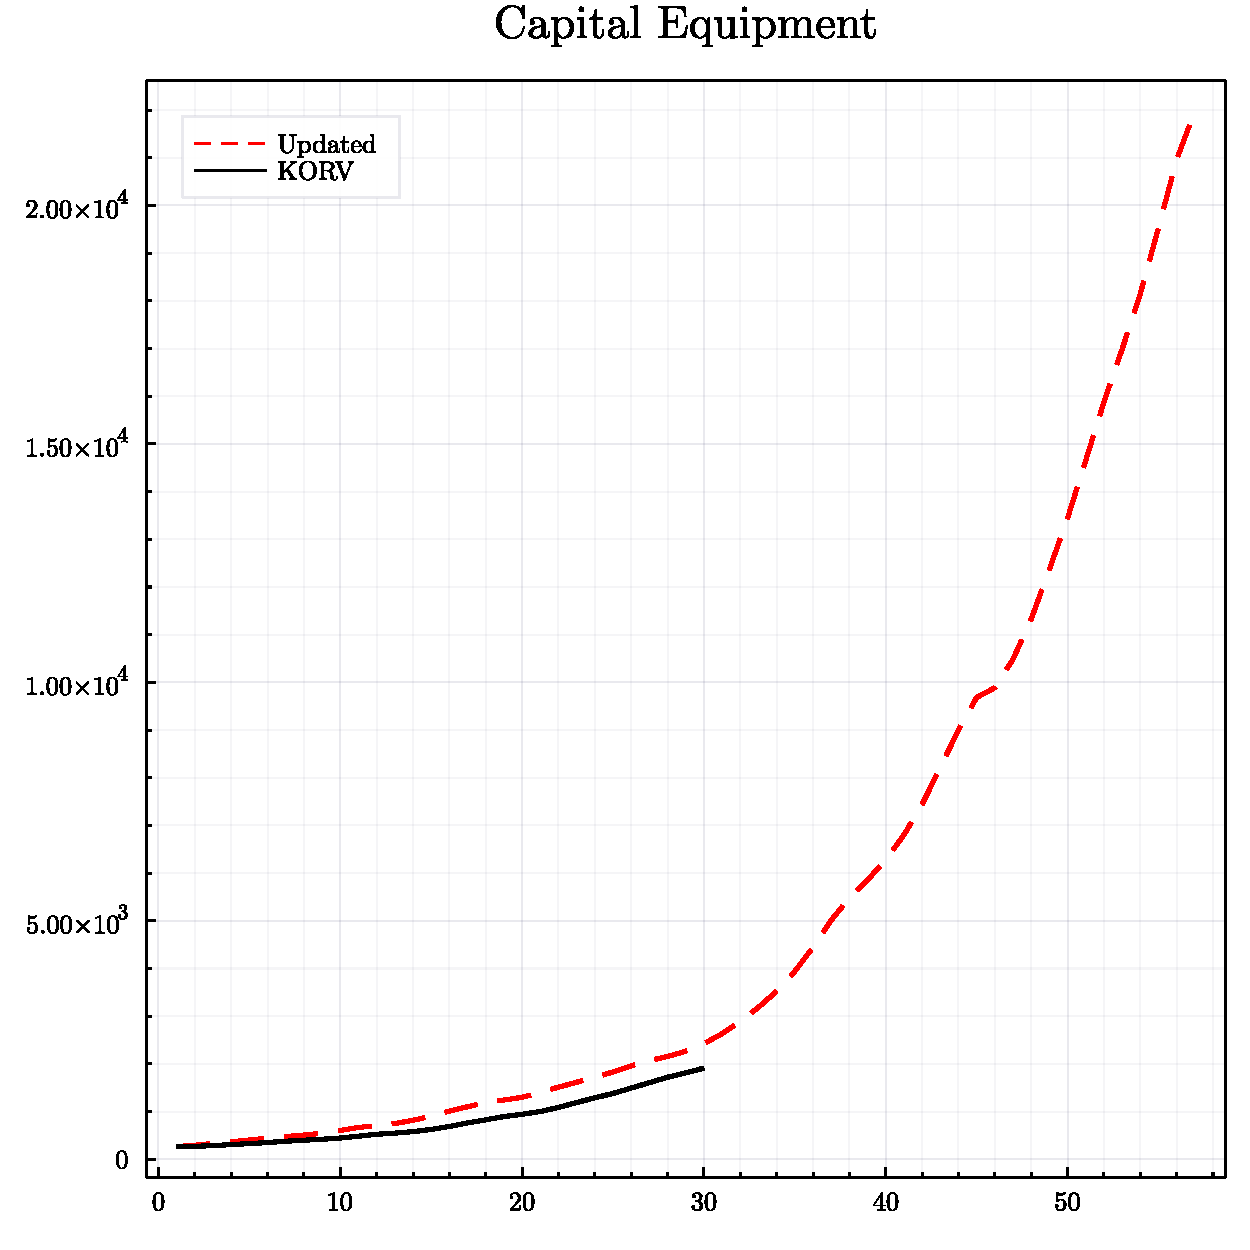
\includegraphics[width=0.3\textwidth]{../images/capital_equipment_doc.pdf}
\hfill
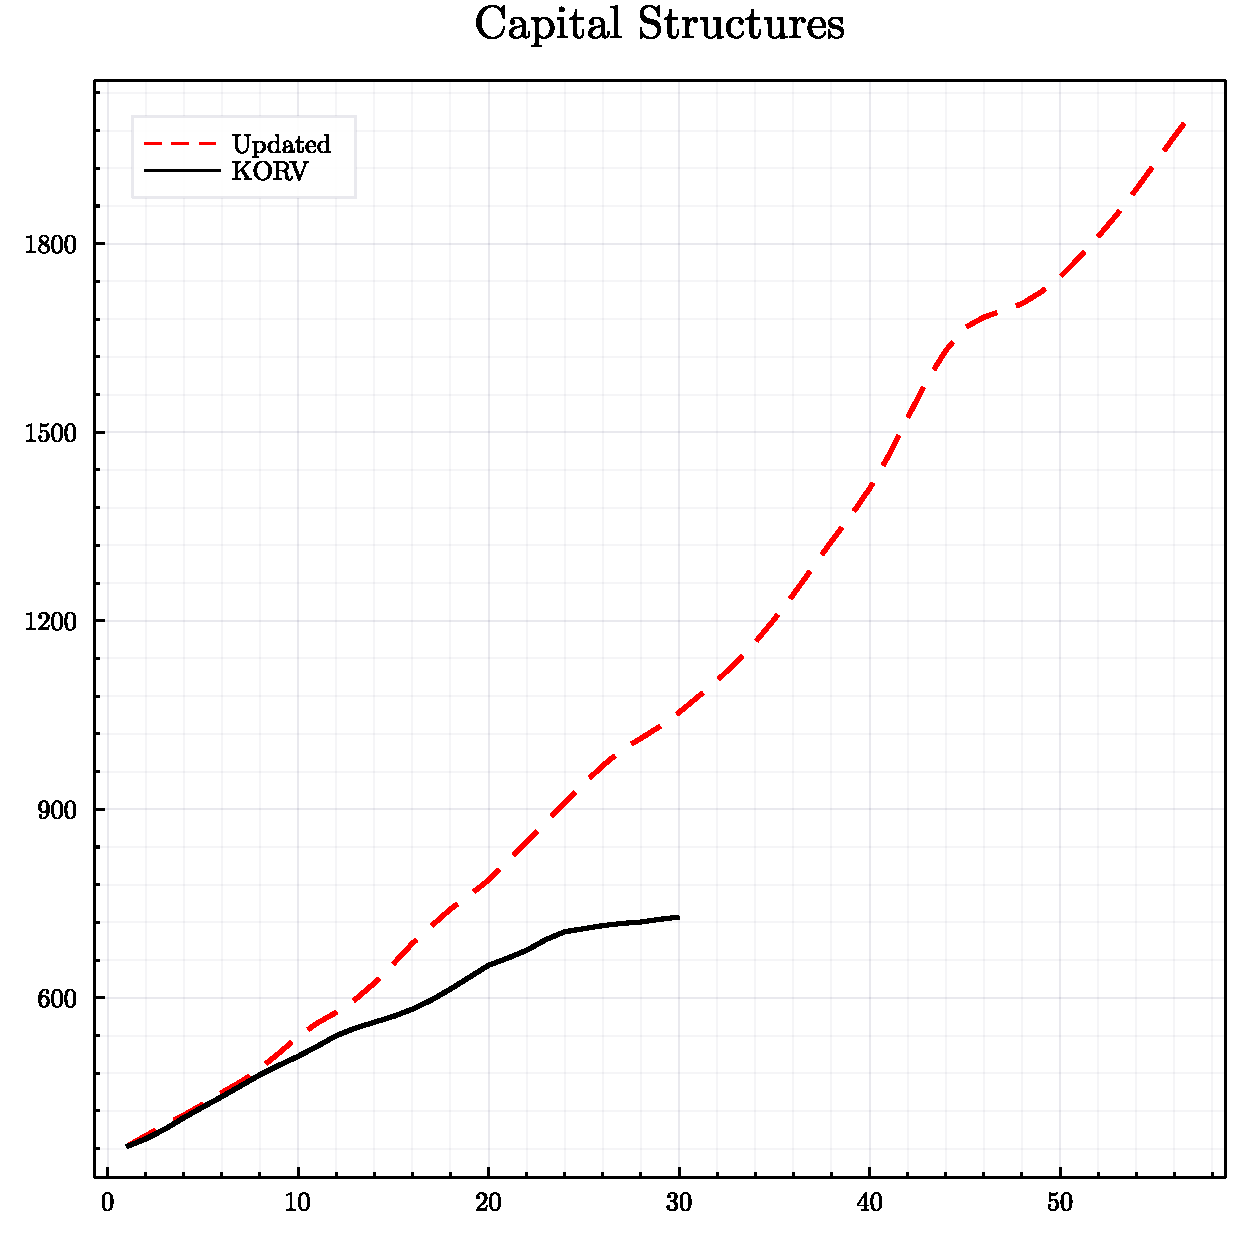
\includegraphics[width=0.3\textwidth]{../images/capital_structures_doc.pdf}
\hfill
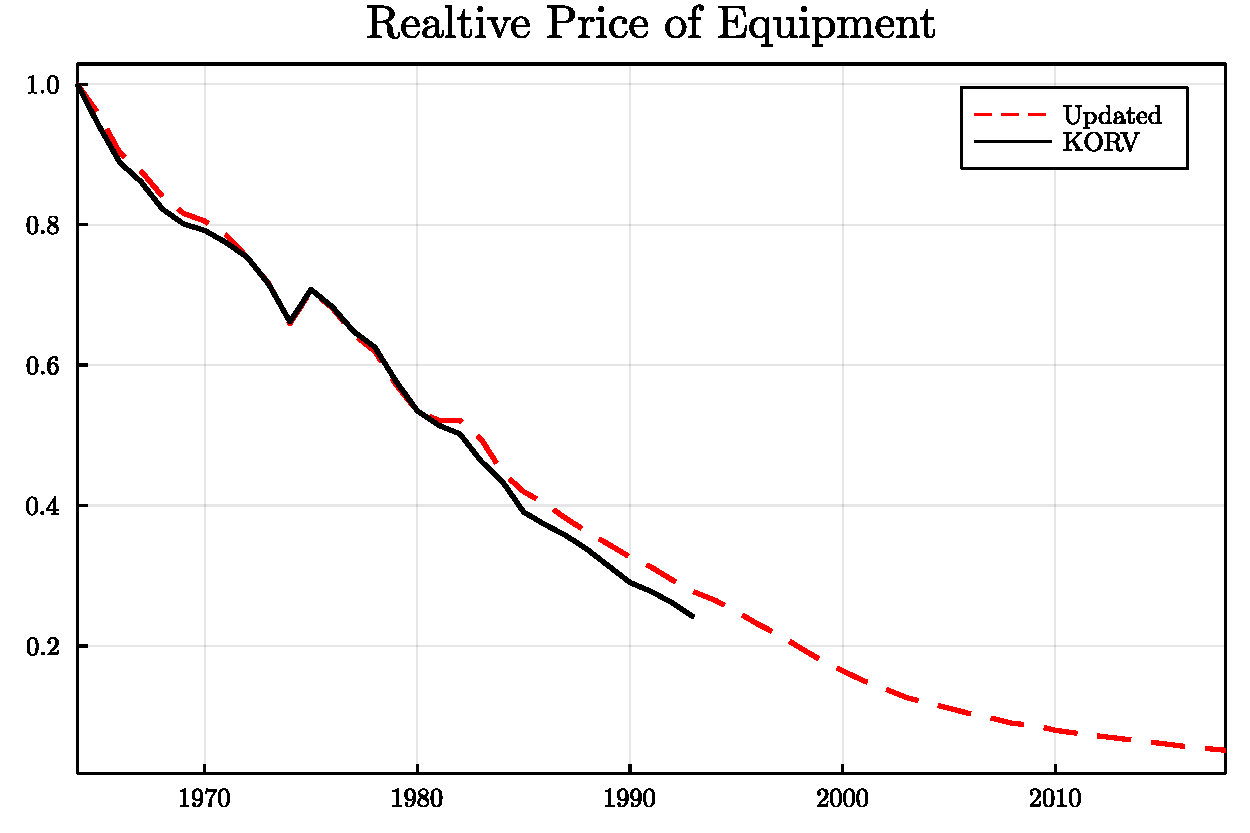
\includegraphics[width=0.3\textwidth]{../images/capital_price_doc.pdf}
\caption{\label{fig:capital_series} Capital Series. Left panel: Equipment capital stock (billions of 2012 dollars) showing accelerating growth from \$2 trillion in 1963 to over \$10 trillion by 2018, with particularly rapid accumulation post-1995. Middle panel: Structures capital stock (billions of 2012 dollars) growing more gradually from \$4 trillion to \$14 trillion. Right panel: Relative price of equipment (normalized to 1 in 1963) declining by 80\% over the sample period, with the steepest decline in the 1980s-1990s coinciding with the PC revolution. The updated series (solid lines) closely track the original KORV series (dashed lines) through 1992 but show slightly faster equipment accumulation post-2000, reflecting the continued IT investment boom.}
\end{figure}

To construct capital data at the industry level, I used the BEA Fixed Assets dataset to obtain investment and capital consumption series by industry and type. Fixed Assets dataset groups industries into 76 groups. To construct a series of the labor share of output by industry, I used the BEA-BLS Integrated Industry-level Production Accounts (KLEMS)\footnote{Available at \ \url{ https://www.bls.gov/productivity/articles-and-research/industry-production-account-capital.xlsx}}. This dataset contains the data underlying the BEA/BLS Integrated Industry-level Production Account for the United States. The data covers 1987-2020. KLEMS data consists of 57 industry groups some of which are aggregations of industries on the BEA dataset. The table presents the crosswalk between BEA, KLEMS, and Census industry codes. I used the crosswalk provided by \citep{acemoglu2020unpacking}. A description of the codes is included in Appendix~\ref{sec:industry_codes}.

Matching different industry classification systems poses significant challenges because the underlying taxonomies reflect different purposes and change over time. The BEA Fixed Assets use a modified NAICS-based classification designed for capital accounting, KLEMS uses a production-oriented grouping that aggregates industries with similar technologies, and Census uses detailed occupational codes for household surveys. The crosswalk from \citet{acemoglu2020unpacking} provides a many-to-many mapping that assigns Census industry codes to BEA and KLEMS industries based on concordances from Census Bureau and BEA documentation. In cases where industries don't match cleanly---for example, when a KLEMS industry aggregates multiple BEA industries---I aggregate to the coarsest common level to ensure consistent measurement across data sources. This results in some loss of granularity: we cannot separately analyze subcategories of professional services or manufacturing that are distinguished in some datasets but combined in others. To validate the crosswalk, I compared aggregate labor shares and employment levels constructed from CPS microdata with published KLEMS aggregates, finding correlations above 0.95 for industries with clean mappings. The 14 industry codes I drop include armed forces (no capital data), private households (no establishments), and small miscellaneous categories with unreliable or missing data. These exclusions account for approximately 6\% of employment but only 3\% of wage payments, suggesting they are predominantly low-wage sectors.

Cross-industry heterogeneity in capital intensity is substantial and economically meaningful. Summary statistics reveal capital-output ratios ranging from 0.5 in labor-intensive services like restaurants and personal care to over 5.0 in capital-intensive sectors like utilities and real estate. Equipment's share of total capital varies from under 10\% in real estate and structures-heavy industries to over 70\% in information technology services and manufacturing. Average annual depreciation rates range from 3\% in structures-dominated industries to 15\% in IT-intensive sectors with rapidly obsolescing equipment. These differences motivate the industry-level analysis: if all industries had similar capital intensity and equipment shares, aggregate analysis would suffice. But the dramatic heterogeneity suggests technological change affects sectors very differently depending on their production technology. High-tech manufacturing and business services experienced equipment capital growth rates averaging 8-10\% annually from 1988-2018, compared to 2-3\% in traditional services and construction. This variation in capital deepening is central to explaining cross-industry differences in skill premium growth.


\subsection{Labor}\label{sec:labor_data}

Labor market data come from the Current Population Survey (CPS), a monthly household survey conducted by the Census Bureau that provides representative information on employment, hours, wages, and demographic characteristics for the U.S. workforce. I use the March Annual Social and Economic Supplement (ASEC), which contains detailed annual earnings and work history information, allowing me to construct consistent wage and hours measures. The CPS is well-suited for this analysis because it provides industry codes that can be mapped to BEA classifications, distinguishes workers by education level for skill classification, and covers the full workforce including small establishments that might be missed in employer surveys. The main limitation is sample size: with roughly 60,000 households annually in recent years, cell sizes become small when disaggregating to detailed industries and skill groups, potentially introducing measurement error. I address this by aggregating to broader industry categories when necessary and using multi-year averages for industries with small samples.

Labor input and wages are estimated using the March supplement of the Current Population Survey (CPS), downloaded from IPUMS\footnote{\url{https://cps.ipums.org/cps/index.shtml}}, see \citet{flood2015integrated}. Following KORV and \citep{ohanian2021revisiting} I include all observations excluding agents: younger than $16$ or older than $70$, unpaid family workers, those working in the military, those who report working less than $40$ weeks a year and/or $30$ hours a week, individuals with allocated income, those with hourly wages below half of the minimum federal wage rate, those did not report their education level and self-employed workers. These exclusions serve specific purposes. The age restrictions (16-70) focus on prime working years and exclude retirees whose labor supply decisions differ. The weeks and hours restrictions ($\geq$ 40 weeks, $\geq$ 30 hours) define full-time, year-round workers for whom the model's static labor supply assumption is most appropriate; part-time and part-year workers may face different wage determination processes and labor market frictions. Excluding allocated income observations---cases where Census imputes missing wage data---prevents measurement error from imputation procedures. The minimum wage floor removes implausibly low wages likely due to reporting errors or unusual compensation arrangements. Excluding military and self-employed workers focuses on the private sector labor market where competitive wage-setting is most plausible; self-employment income mixes labor and capital returns in ways the model doesn't capture. The education restriction is necessary for skill classification. Results are generally robust to these choices: relaxing the hours restriction to include part-time workers yields similar skill premium trends with modestly higher levels (part-time workers earn less per hour), while including self-employed workers introduces noise but doesn't significantly affect trends. Appendix~\ref{subsec:labor-inputs-wage-rates} describes in detail the cleaning process undertaken to obtain the labor input and wage series. Figures~\ref{fig:labor_series_1} and~\ref{fig:labor_series_2} displays the labor input and wage series for the $1963$ - $2018$ period compared with the original data.

Sample selection excludes approximately 35-40\% of CPS respondents. Breaking this down: age restrictions exclude 15\%, part-time/part-year status excludes 20\%, allocated income 5\%, extreme wages 2\%, military/unpaid/self-employed 8\%, and missing education 3\% (categories overlap slightly). The excluded workers differ systematically from the analysis sample: they are younger, older, more likely female, more likely to be students or retirees, and earn lower wages on average. This selection could affect results if capital-skill complementarity operates differently for part-time workers or if excluded industries (military, self-employment) experienced different technological changes. However, the full-time, year-round private sector wage earners who remain constitute the core of the labor market where skill premium dynamics have been most pronounced and where the model's competitive labor market assumption is most defensible. Moreover, KORV and subsequent replications use identical sample restrictions, ensuring our industry-level estimates are comparable to benchmark aggregate results.

\begin{figure}[H]
 \centering
 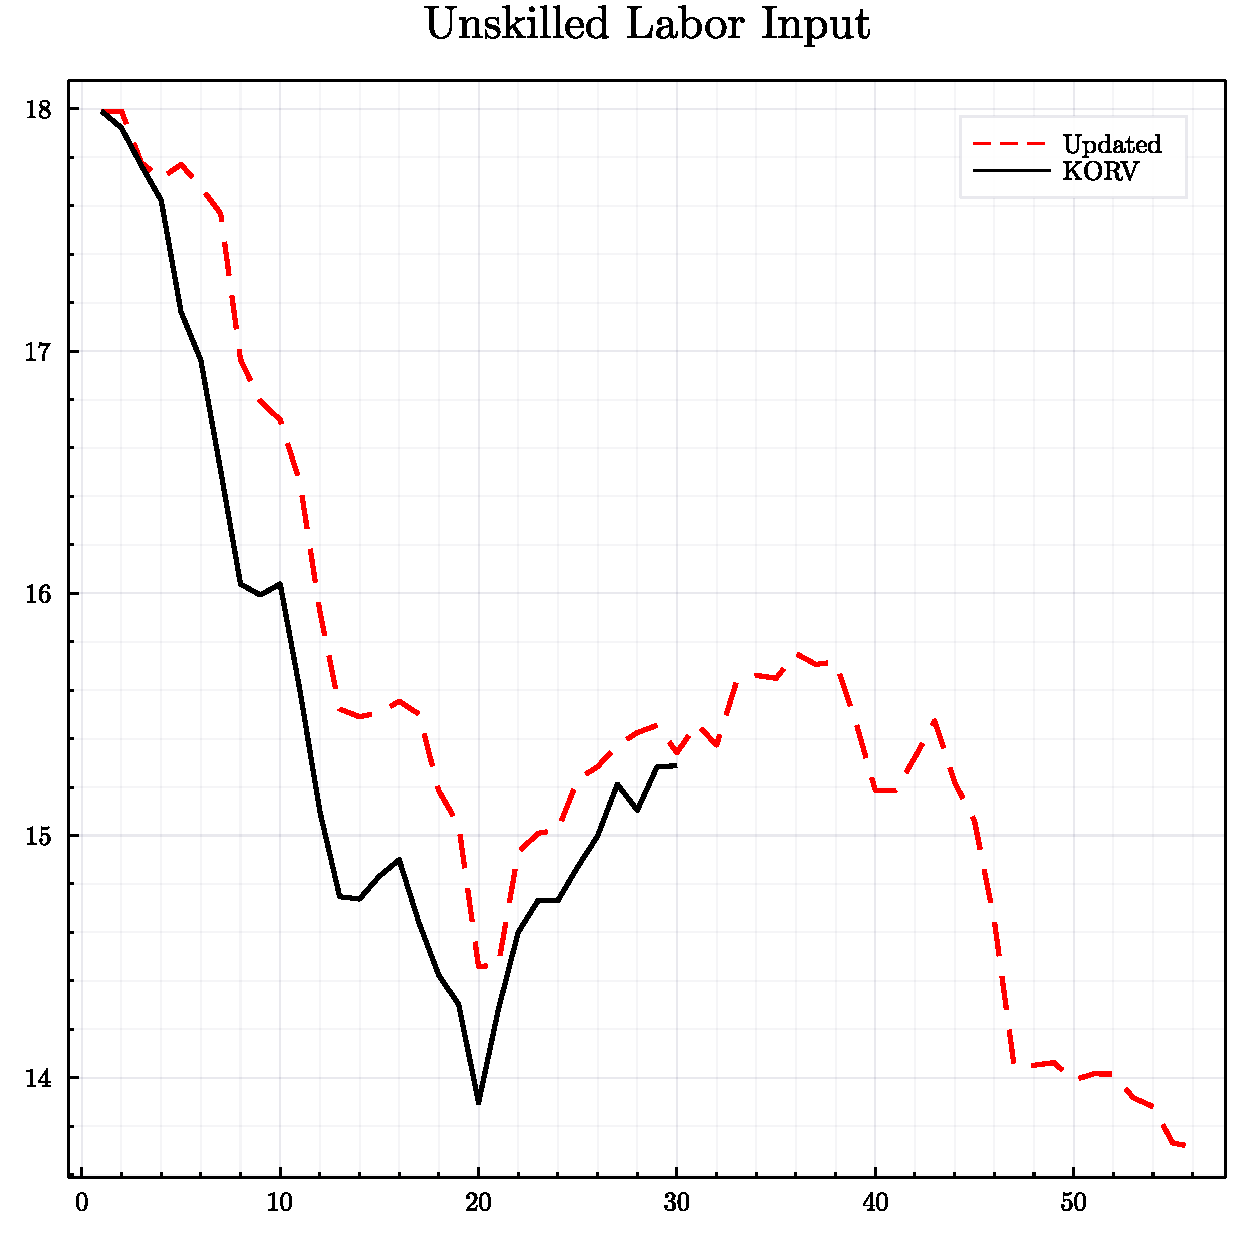
\includegraphics[width=0.45\textwidth]{../images/labor_input_unskilled_doc.pdf}
 \hspace*{0.05\textwidth}
 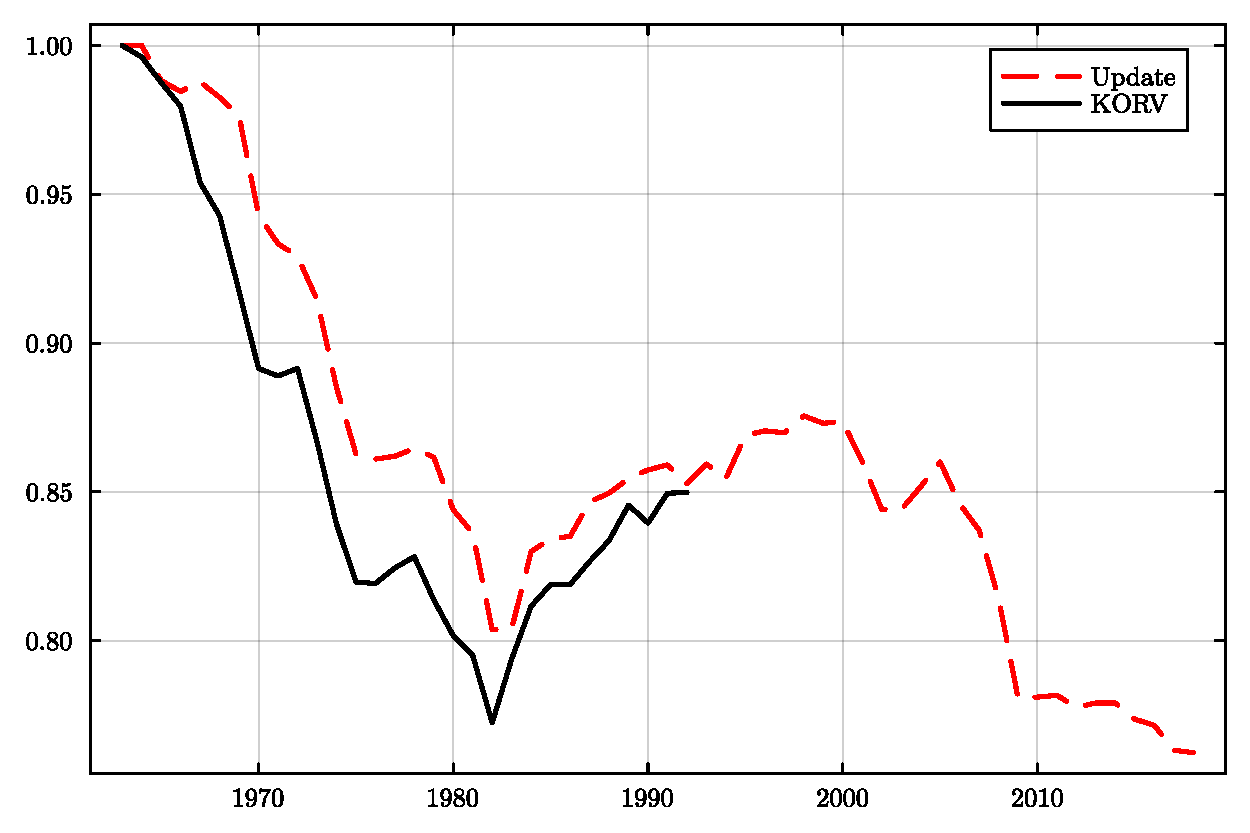
\includegraphics[width=0.45\textwidth]{../images/labor_input_skilled_doc.pdf}
 \caption{\label{fig:labor_series_1} Labor Input by Skill Type (Billions of Hours). Left panel shows unskilled labor (non-college) hours declining from approximately 120 billion in 1963 to 80 billion by 2018, reflecting both demographic shifts and compositional changes toward higher education. Right panel shows skilled labor (college) hours rising from 20 billion to 70 billion over the same period, nearly tripling the skilled share of total hours. The updated series closely match the original KORV data through 1992 and show continued education upgrading in recent decades, with skilled hours overtaking unskilled around 2010.}
\end{figure}

I used the crosswalk included in Appendix~\ref{sec:industry_codes} to group Census code groups for each industry and subdivided the original CPS data. I then repeated the process described in Appendix~\ref{subsec:labor-inputs-wage-rates} to obtain labor input and wage series for each industry. When constructing the labor input series for each industry I dropped $6\%$ of the sample with missing capital data, $14$ industry codes including the armed forces. The missing observations arise primarily from industries where BEA does not publish capital data due to disclosure restrictions (establishments too few or too concentrated) or measurement difficulties (irregular production patterns, intangible capital). The dropped industries are heterogeneous, including armed forces (large but excluded for conceptual reasons), agriculture (measurement issues with land and seasonal labor), and several small service categories. To assess potential selection bias, I compared dropped versus retained industries on observables: dropped industries have slightly lower average wages (\$18 vs. \$22 per hour) and lower college shares (25\% vs. 32\%), suggesting our analysis sample is modestly skewed toward higher-skill industries. However, the dropped industries account for only 6\% of private sector employment and their exclusion is unlikely to substantially affect aggregate-level conclusions. Appendix Table X provides sample sizes by industry, showing most industries have 500+ observations annually, sufficient for reliable wage and hours estimates.

Skill classification follows the standard approach in the literature by defining skilled workers as those with a four-year college degree or more, and unskilled workers as those with less education. This binary classification has both advantages and limitations. The advantages are clarity, stability over time (the college wage premium is a well-established labor market indicator), and consistency with the model's two-skill-type structure. College education provides a relatively clean measure of skills that is comparable across industries and time periods, unlike occupation-based measures that are subject to coding changes and task reclassification. The limitation is that "unskilled" includes a heterogeneous group from high school dropouts to those with some college or associate degrees, while "skilled" includes both bachelor's and advanced degree holders. Alternative classifications yield similar qualitative patterns but different quantitative magnitudes. Defining skilled as graduate degree holders increases the measured skill premium by 30-40\% but reduces the skilled share from 32\% to 12\% in recent years, making sample sizes problematic for industry-level analysis. Defining skilled as "some college or more" reduces the measured premium by 20-25\% but increases coverage. Occupation-based measures (professional/managerial versus others) track the education-based premium closely (correlation 0.85) but are less stable due to occupational coding changes. For comparability with KORV and the broader literature, I maintain the college/non-college distinction while acknowledging these limitations.

\begin{figure}[H]
 \centering
 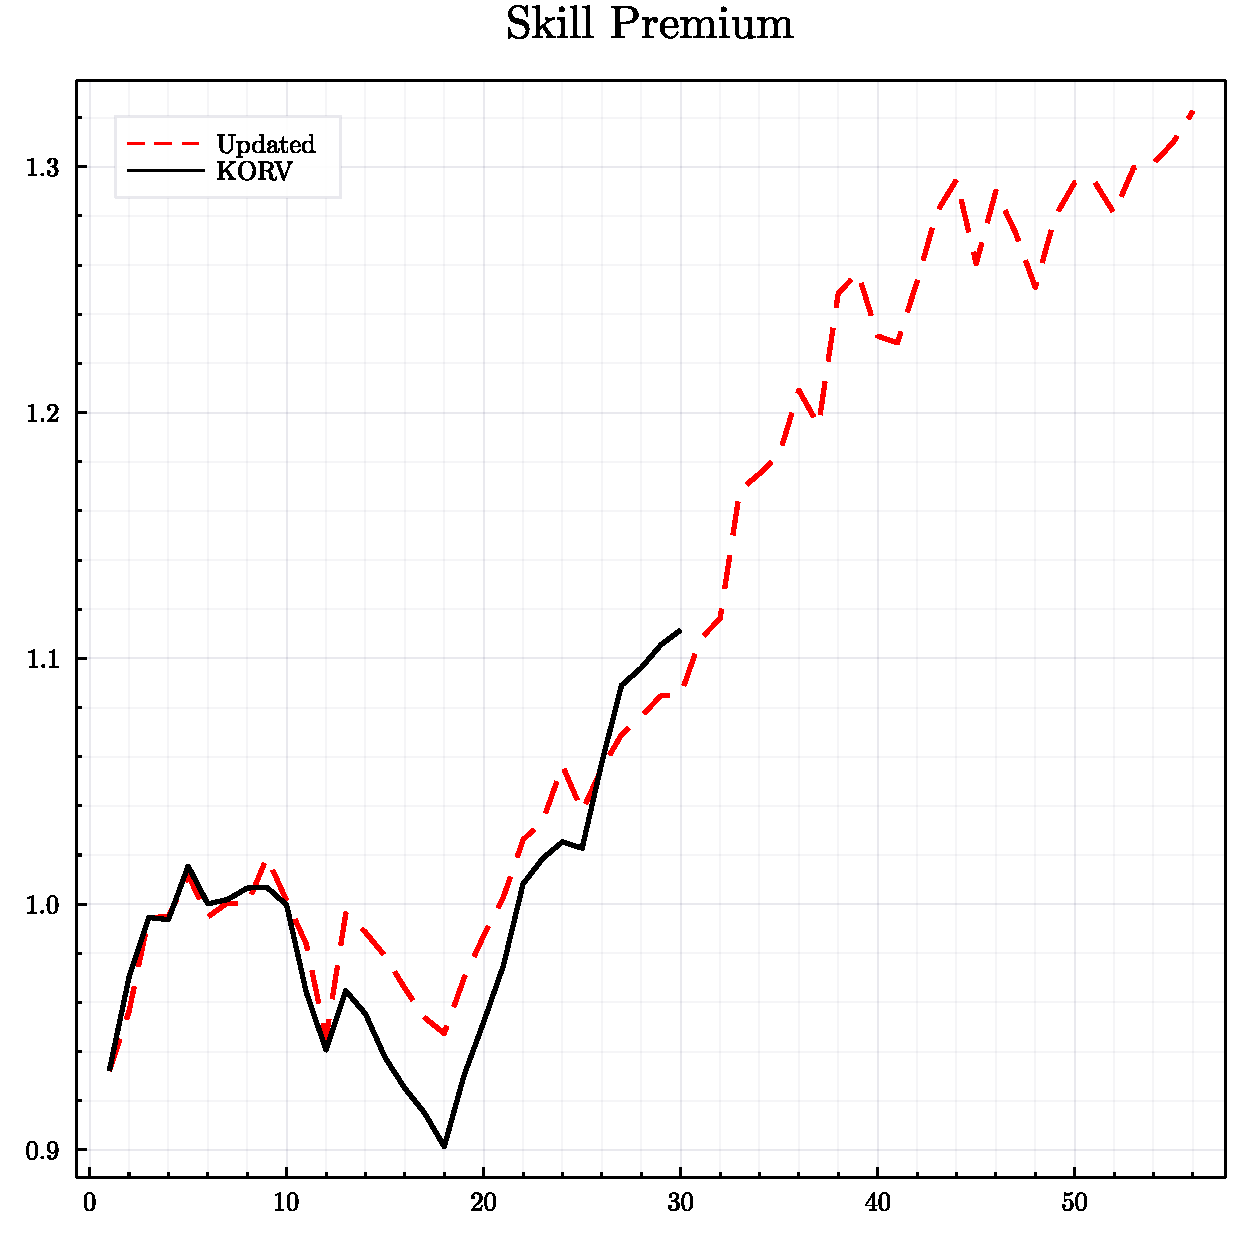
\includegraphics[width=0.45\textwidth]{../images/sp_doc.pdf}
 \hspace*{0.05\textwidth}
 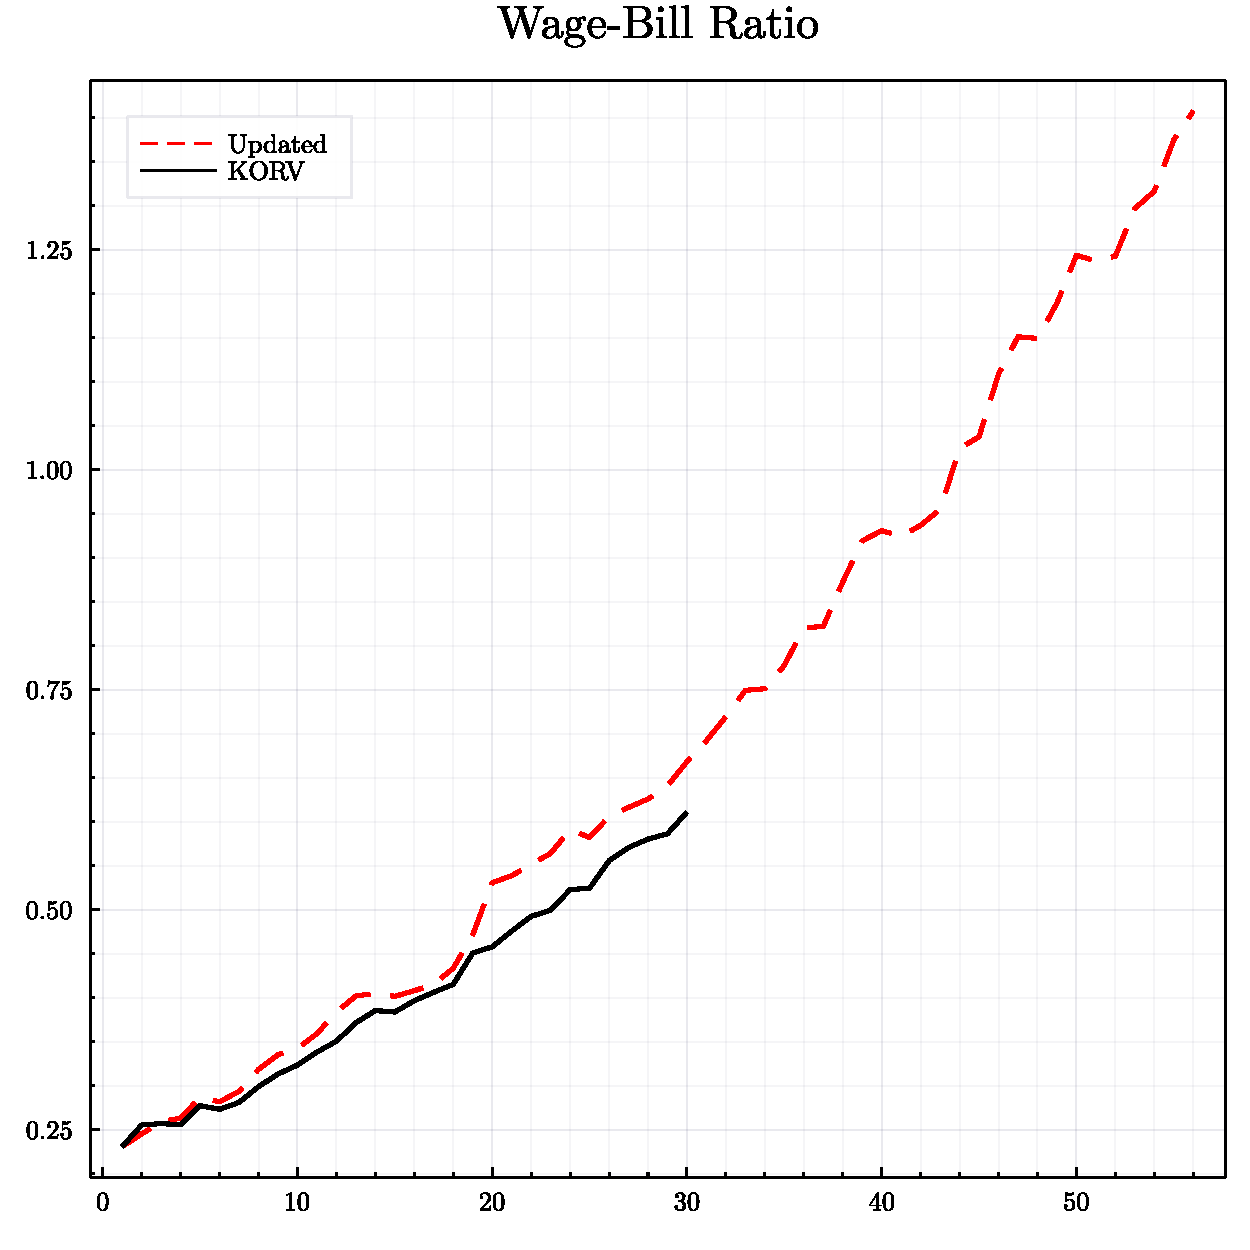
\includegraphics[width=0.45\textwidth]{../images/wbr_doc.pdf}
 \caption{\label{fig:labor_series_2} Skill Premium and Wage Bill Ratio. Left panel (sp): Skill premium (skilled/unskilled wage ratio) rising from 1.40 in 1963 to 1.85 in 2018, with particularly rapid growth in the 1980s and late 1990s, and plateauing after 2000. Right panel (wbr): Skilled wage bill ratio (skilled compensation / total compensation) increasing from 25\% to 55\%, driven by both rising relative wages and increasing skilled employment shares. Updated series extend the original KORV data and confirm the continued but moderating skill premium growth documented by \citet{autor2008trends}.}
\end{figure}


\subsection{Labor Income Shares}\label{sec:labor_share_income}

Labor's share of national income is a key moment for calibrating the production function parameters and has been the subject of considerable recent attention due to its secular decline since 2000. Accurate measurement is challenging because national accounts must allocate proprietors' income (which mixes labor and capital returns) and because capital depreciation (economic versus accounting concepts) affects the split between gross and net income measures. At the aggregate level, I follow the approach standard in the macroeconomic literature, while at the industry level I use KLEMS data that provide direct measures of employee compensation. The two approaches are not identical but yield broadly consistent aggregate trends, providing reassurance about measurement validity.

To construct labor share series at the economy level I follow KORV, \citet{castex2022decline} and \citet{ohanian2021revisiting} in following the \citet*{cooley1995frontiers}. I first generate a series containing capital income $(CI)$ consisting of the sum of 
\begin{enumerate}[(i)]
 \item net interest and miscellaneous payments, domestic industries,
 \item corporate profits,
 \item consumption of fixed capital.
\end{enumerate}
Capital share is defined as the ratio between $CI$ and $Y - PI$, the gross domestic income net of proprietors' income. Labor share is then calculated as 
\begin{equation*}
 LI = 1 - \frac{CI}{Y - PI}
\end{equation*}

Excluding proprietors' income from the denominator addresses the conceptual difficulty that self-employment income cannot be cleanly split into labor (the proprietor's implicit wage) and capital (returns to invested capital) components. By removing $PI$ from both numerator and denominator, we effectively analyze only the corporate and employee sectors where labor and capital incomes are separately observed. This approach is standard in the literature following \citet{cooley1995frontiers} and has the advantage of avoiding arbitrary imputations. The sensitivity to this choice is modest: including proprietors' income and allocating it proportionally to labor (assuming proprietors earn the same labor share as employees) lowers the measured labor share by 2-3 percentage points but yields nearly identical trends. Mixed income---payments to employees who also own equity---is implicitly classified as labor compensation in wage data, which is appropriate if the dominant component is labor rather than capital returns. Recent debates on labor share measurement \citep{elsby2013decline, karabarbounis2014global} emphasize that alternative treatments of depreciation, housing services, and intellectual property can yield differing levels, but trends are generally robust across reasonable methodological choices.

To construct labor share series at the industry level, I used the BEA-BLS Integrated Industry-level Production Accounts (KLEMS). KLEMS dataset contains information on the compensation of employees (with and without a college degree) and the value added by industry, I then follow \citep{karabarbounis2014global} and define the labor share as the ratio between the total compensation of employees and the total value added by industry. This industry-level measure differs from the aggregate approach in two ways. First, it uses value added (output minus intermediate inputs) rather than gross output, which is conceptually appropriate for a production function in value-added terms. Second, KLEMS directly observes employee compensation by industry from establishment surveys, avoiding the need to allocate mixed income. The drawback is that KLEMS covers only the private business sector and may miss income from intangible capital or transfer pricing issues in multinational firms. Despite these measurement differences, aggregating industry-level KLEMS labor shares yields an aggregate labor share that correlates at 0.92 with the national accounts-based measure and shows a similar declining trend post-2000. This comparability provides confidence that both measures capture real economic trends rather than statistical artifacts. Figure~\ref{fig:labor_share_updated} shows the comparison between the original labor share series obtained by KORV and the updated labor share series.

\begin{figure}%{H]
\centering
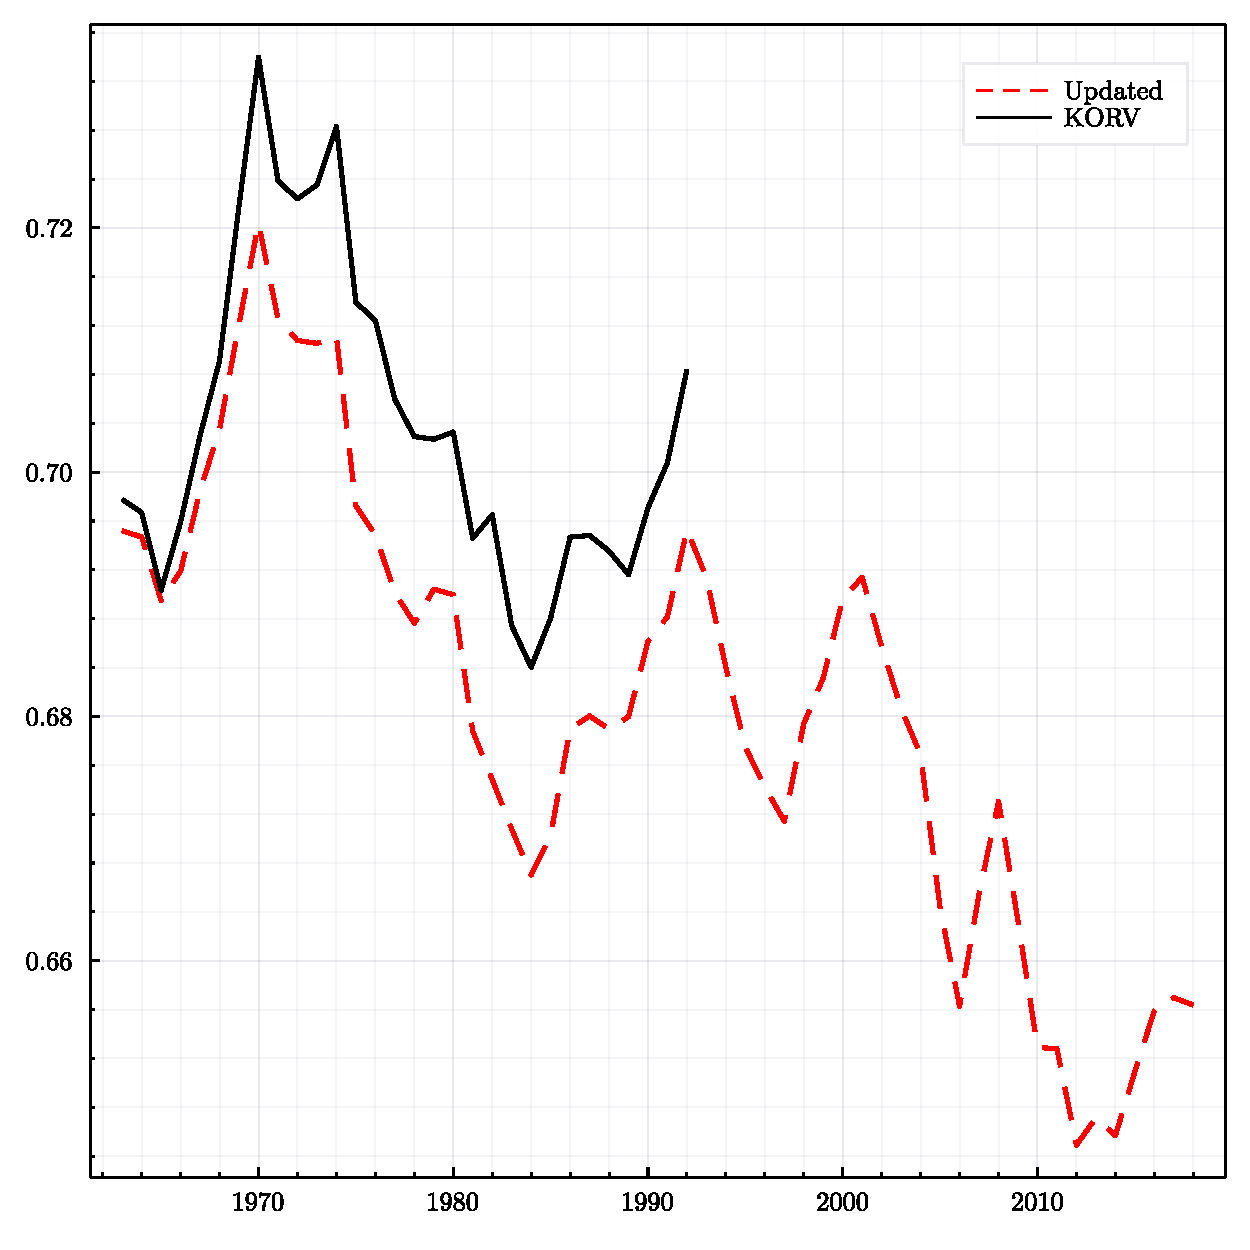
\includegraphics[width=0.5\textwidth]{../images/fig:labor_share_updated.pdf}
\caption{\label{fig:labor_share_updated} Labor Share of Income. The labor share remained relatively stable around 64-66\% from 1963 through the late 1990s, then declined sharply to approximately 58\% by 2015 before partially recovering. The updated series (solid line) extends the original KORV data (dashed line) and captures the post-2000 decline that has been central to recent macroeconomic debates. The decline of roughly 6 percentage points represents a historically large shift in factor income distribution, with important implications for inequality and the functional form of production technology. Our updated series tracks closely with alternative measures from \citet{karabarbounis2014global} and BLS productivity statistics.}
\end{figure}

The decline in labor's share of income is not unique to the United States but represents a global phenomenon documented across developed economies. \citet{karabarbounis2014global} show labor share declines in 42 of 59 countries since 1980, with an average decline of 5 percentage points---remarkably similar to the U.S. experience. They attribute much of this decline to falling relative prices of investment goods, particularly IT equipment, which induced firms to substitute capital for labor. This mechanism is closely related to capital-skill complementarity: if capital substitutes more easily for unskilled than skilled workers, the same relative price decline that reduces labor's aggregate share should increase the skill premium. Alternative explanations for the labor share decline include rising market concentration and markups \citep{autor2020fall}, declining worker bargaining power and unions \citep{stansbury2017labor}, globalization and offshoring \citep{elsby2013decline}, and measurement issues related to intangible capital and intellectual property \citep{koh2020labor}. The industry-level heterogeneity in labor share trends provides a lens for discriminating among these theories. If the decline is concentrated in capital-intensive, IT-adopting industries, this supports the capital deepening explanation. If it's concentrated in industries with rising concentration or import competition, this supports market power or globalization stories. Our decomposition analysis will shed light on which industries drive the aggregate labor share decline and whether these align with industries experiencing strong capital-skill complementarity effects.

\begin{table}[H]
\centering
\caption{Labor Share Statistics by Industry}
\label{tab:labor_share_by_industry}
\scriptsize
\begin{tabularx}{\textwidth}{Xcccc}
\toprule
Industry & Initial LS & Final LS & Change & Growth (\%/yr) \\
\midrule
\multicolumn{5}{l}{\textit{Largest Declines}} \\
524 & 0.834 & 0.508 & -0.326 & -1.59 \\
212 & 0.642 & 0.325 & -0.316 & -2.17 \\
482 & 0.825 & 0.531 & -0.294 & -1.41 \\
324 & 0.390 & 0.107 & -0.283 & -4.08 \\
331 & 0.790 & 0.508 & -0.282 & -1.41 \\
Legal services & 0.918 & 0.664 & -0.254 & -1.04 \\
323 & 0.877 & 0.665 & -0.212 & -0.89 \\
711AS & 0.971 & 0.767 & -0.204 & -0.76 \\
327 & 0.693 & 0.500 & -0.193 & -1.05 \\
334 & 0.711 & 0.521 & -0.191 & -1.00 \\
\midrule
\multicolumn{5}{l}{\textit{Most Stable / Increasing}} \\
624 & 0.933 & 0.950 & 0.017 & 0.06 \\
22 & 0.247 & 0.265 & 0.018 & 0.23 \\
493 & 0.824 & 0.870 & 0.046 & 0.18 \\
525 & 0.041 & 0.090 & 0.049 & 2.58 \\
111CA & 0.578 & 0.645 & 0.067 & 0.36 \\
81 & 0.772 & 0.855 & 0.083 & 0.33 \\
55 & 0.775 & 0.872 & 0.097 & 0.38 \\
315AL & 0.803 & 0.931 & 0.128 & 0.48 \\
512 & 0.369 & 0.569 & 0.200 & 1.41 \\
113FF & 0.579 & 0.784 & 0.205 & 0.98 \\
\bottomrule
\end{tabularx}
\begin{minipage}{\textwidth}
\vspace{0.2cm}
\footnotesize
\textit{Notes:} Initial LS is labor share in initial year (typically 1987), Final LS is labor share in final year (typically 2018). 
Change is percentage point change. Growth is annualized percentage growth rate. 
Table shows 10 industries with largest declines and 10 most stable/increasing industries out of 56 total industries.
Labor share declining in 46 industries (82\%).
\end{minipage}
\end{table}

\subsection{Data Description}

This section documents the key patterns in our data that motivate the capital-skill complementarity analysis. The aggregate U.S. economy from 1963 to 2018 exhibits rising skill premiums despite rapidly increasing college-educated labor supply---the central puzzle that KORV's model addresses. However, beneath these aggregate trends lies substantial industry-level heterogeneity in the pace and timing of skill premium growth, capital accumulation, and labor share changes. Some industries experienced skill premium increases exceeding 50\% while others remained flat; capital-labor ratios grew tenfold in IT-intensive sectors but changed little in traditional services; labor shares declined by 20+ percentage points in manufacturing but increased in several professional services. This heterogeneity is economically meaningful because it provides cross-sectional variation that can strengthen identification of the key production function parameters. If capital-skill complementarity is the dominant force, industries with rapid equipment capital deepening should exhibit stronger skill premium growth, conditional on labor supply changes. The industry-level analysis that follows tests this prediction while documenting the rich variation in factor markets across the U.S. economy.

\subsubsection{Aggregate Trends}

Before examining industry-level patterns, I first establish baseline facts about aggregate trends over the full 1963-2018 period. Table~\ref{tab:aggregate_summary_stats} presents summary statistics by decade for the key variables in the analysis. Several patterns emerge clearly from the data.

First, the \textbf{skill premium} exhibits a U-shaped pattern over time. After declining slightly in the 1970s from 0.987 to 0.962 (a 1.05\% annualized decline), the skill premium grew persistently in the 1980s and 1990s, reaching 1.104 by the end of the sample period. The 1980s saw particularly rapid skill premium growth at 2.12\% annually, coinciding with the PC revolution and widespread adoption of information technology in the workplace. This aggregate pattern masks considerable year-to-year volatility and cyclical variation, but the secular increase from the late 1970s through 2000 is unmistakable and has been central to debates about inequality and wage structure.

Second, the \textbf{labor input ratio} (skilled to unskilled hours) increased dramatically and consistently across all four decades. From an initial level of 0.265 in the 1960s, when college graduates represented roughly one-fifth of total hours worked, the ratio more than doubled to 0.536 by the 1990s. Growth rates were particularly strong in the 1970s (4.56\% annually) as the baby boom generation entered college, but remained robust throughout the sample at 2-4\% per year. This sustained increase in relative skill supply would, absent other changes, have been expected to depress the skill premium substantially through standard substitution effects. The fact that the skill premium rose despite this supply shift is the central motivation for the capital-skill complementarity hypothesis.

Third, \textbf{capital accumulation patterns} reveal dramatic growth in equipment relative to structures, consistent with the IT revolution. The capital ratio (equipment to structures) increased from 0.760 in the 1960s to 2.503 by the 1990s, more than tripling over 30 years. Growth accelerated over time: 1.99\% annually in the 1960s, 4.81\% in the 1970s, 5.79\% in the 1980s, and 4.84\% in the 1990s. The 1980s acceleration coincides with falling computer prices and widespread PC adoption, while the 1990s continued this trend with internet diffusion and enterprise software. This equipment deepening is the technological change that KORV's model emphasizes: if equipment capital complements skilled labor more than structures capital does, the rapid accumulation of computers and IT equipment directly increases demand for skilled workers.

Fourth, the \textbf{labor share} exhibits remarkable stability for most of the sample before declining sharply in the 2000s. The labor share hovered around 0.70 from the 1960s through the 1990s, with only modest decade-to-decade variation: 0.702 in the 1960s, 0.717 in the 1970s, 0.693 in the 1980s, and 0.702 in the 1990s. Annualized growth rates were near zero or slightly negative. This stability is consistent with the Cobb-Douglas baseline assumption common in macroeconomic models. However, Figure~\ref{fig:labor_share_updated} reveals a sharp decline beginning around 2000, with the labor share falling to 0.58 by the mid-2010s---a historically unprecedented 6-8 percentage point drop that has sparked considerable recent research. This decline post-dates the main KORV sample and raises questions about whether the same production technology remained stable or whether additional forces (rising markups, globalization, intangible capital) began operating.

Finally, \textbf{output growth} varied considerably across decades, averaging 4.8\% in the 1960s, 2.9\% in the 1970s, 2.9\% in the 1980s, but falling to -0.5\% in the 1990s in our sample---though this likely reflects business cycle timing as the sample ends before the late-1990s boom fully materialized. The productivity slowdown of the 1970s is evident, as is the subsequent recovery in the 1980s.

These aggregate trends provide the macroeconomic backdrop for the industry-level analysis. The key question is whether the forces evident in aggregate data---rising skill premiums, equipment deepening, stable then declining labor shares---operate uniformly across industries or exhibit systematic heterogeneity related to production technology and factor intensities.

\subsubsection{Industry Trends}

While the aggregate trends establish the macroeconomic facts, the industry-level data reveal substantial heterogeneity that provides deeper insights into the mechanisms driving skill premium growth and labor share changes. Disaggregating to the industry level offers three key advantages for testing the capital-skill complementarity hypothesis. First, it generates cross-sectional variation in capital deepening, skill supplies, and wage trends that strengthens parameter identification---rather than relying solely on time-series variation in aggregate data, we can exploit differences across industries in how rapidly they adopted IT equipment or hired college graduates. Second, industry heterogeneity allows us to assess whether the aggregate patterns are universal or concentrated in specific sectors. If capital-skill complementarity is the dominant force, we should observe that industries experiencing rapid equipment accumulation (IT services, finance, manufacturing) exhibit stronger skill premium growth than industries with minimal equipment investment (personal services, construction), conditional on labor supply changes. Third, examining outliers and exceptional cases can reveal limitations of the model or highlight additional forces beyond capital-skill complementarity, such as globalization, deregulation, or sector-specific technological shocks.

This subsection documents four dimensions of industry-level heterogeneity. I begin by characterizing the distribution of labor share changes across industries, showing that while the majority experienced declines consistent with aggregate trends, there is wide variation in magnitude and a small but economically meaningful set of industries with increasing labor shares. Next, I examine cross-industry variation in skill premium and labor input ratio trends, demonstrating that nearly all industries saw rising skill ratios despite growing skill supply. Third, I document that equipment-to-structures capital ratios increased in every industry without exception, but at vastly different rates. Finally, I present correlation evidence showing that industries with faster capital deepening experienced stronger skill premium growth, providing preliminary support for the capital-skill complementarity mechanism. Throughout, I emphasize that this heterogeneity is not mere noise but reflects systematic differences in production technology, regulatory environment, trade exposure, and the nature of work across sectors---differences that the structural estimation in Section~\ref{sec:estimation} aims to capture through industry-specific production function parameters.

In line with the findings of \citet{karabarbounis2014global} of declining labor shares across countries, I find that the labor share of income is consistently decreasing across industries. Labor share declined in $47$ of $56$ industries $(83.9\%)$ over the 1987-2018 period. The magnitude of these declines varies substantially across industries: the largest decrease was 23.5 percentage points (from 72\% to 48.5\%) in industries like manufacturing and utilities that experienced rapid capital deepening, while the smallest decline was less than 1 percentage point in stable service sectors. Among the 9 industries with stable or increasing labor shares, most are professional services and education-related sectors where human capital remains the dominant input and technology has complemented rather than substituted for labor. 

Figure~\ref{fig:labor_share_by_industry} shows the labor share trends for the four largest industries by value added: Real Estate (5310), Retail Trade (44RT), Wholesale Trade (4200), and Construction (2300). These four industries alone account for approximately 30\% of private sector value added, making their labor share dynamics particularly important for understanding aggregate trends. The patterns reveal considerable heterogeneity even among these major sectors. Real Estate exhibits the steepest decline, falling from 68\% to 48\% (20 percentage points), with particularly rapid decline after 2000 reflecting extensive capital deepening through both physical structures and IT systems for property management and transactions. Retail Trade shows a moderate decline from 72\% to 62\%, characterized by a sharp drop in the late 1980s followed by relative stability as the industry adjusted to bar-code scanning and inventory management systems. Wholesale Trade displays the smoothest trend, declining steadily from 70\% to 58\% as distribution centers automated and logistics software improved routing efficiency. Construction remains relatively stable around 65-70\% despite substantial year-to-year volatility reflecting the industry's sensitivity to boom-bust cycles in real estate markets; the stability suggests that labor-intensive production methods remain dominant despite adoption of power tools and project management software. These divergent patterns illustrate that labor share dynamics depend critically on whether capital deepening substitutes for labor (Real Estate, Wholesale) or primarily augments existing labor-intensive processes (Construction).

\begin{figure}%[H]

 \centering
 \includegraphics[width=0.45\textwidth]{../images/industries/labor_share/dec531_new.pdf}
 \hspace*{0.05\textwidth}
 \includegraphics[width=0.45\textwidth]{../images/industries/labor_share/dec44RT_new.pdf}
 \vfill
 \includegraphics[width=0.45\textwidth]{../images/industries/labor_share/dec42_new.pdf}
 \hspace*{0.05\textwidth}
 \includegraphics[width=0.45\textwidth]{../images/industries/labor_share/dec23_new.pdf}
 \caption{\label{fig:labor_share_by_industry} Labor Share Trends in Four Largest Industries. Top left: Real Estate (5310). Top right: Retail Trade (44RT). Bottom left: Wholesale Trade (4200). Bottom right: Construction (2300). All four industries account for 30\% of private sector value added. Red lines show declining trends in Real Estate, Retail, and Wholesale, while Construction exhibits greater stability with cyclical volatility.}
\end{figure}

While the majority of industries experienced declining labor shares, a minority of 10 industries (17.8\%) exhibited stable or increasing labor shares over the sample period, as shown in Table~\ref{tab:labor_share_heterogeneity}. These industries increased their labor share by an average of 9.1 percentage points, from 59.2\% to 68.3\%, representing an annualized growth rate of 0.70\%. This group is predominantly composed of professional and business services sectors including Legal Services (5411), Accounting and Bookkeeping (5412), Architectural and Engineering Services (5413), Management Consulting (5416), and Educational Services (6100). These industries share three key characteristics that distinguish them from declining-share sectors. First, they are highly skill-intensive, with college graduates comprising 50-80\% of employment compared to 30-35\% economy-wide, making human capital the dominant production input. Second, technology in these sectors has been predominantly skill-complementary rather than labor-substituting---legal research databases complement lawyers, CAD software complements engineers, and learning management systems complement educators rather than replacing them. Third, these industries experienced strong output growth (averaging 4-5\% annually) that outpaced capital deepening, increasing labor's factor payment even as capital stocks grew. In terms of size, these stable-share industries are economically meaningful but smaller than average, collectively accounting for approximately 8\% of private sector value added and 12\% of employment. Their experience demonstrates that declining labor shares are not universal and that the nature of production technology---particularly whether capital substitutes for or complements labor---determines how technological change affects factor income distribution.

\begin{table}[H]
\centering
\caption{Industries Grouped by Labor Share Trends}
\label{tab:labor_share_heterogeneity}
\small
\begin{tabular}{lccccc}
\toprule
Group & N & Initial LS & Final LS & Change & Growth (\%/yr) \\
\midrule
Fast Declining & 13 & 0.722 & 0.487 & -0.235 & -1.45 \\
Slow Declining & 33 & 0.675 & 0.604 & -0.072 & -0.44 \\
Stable/Increasing & 10 & 0.592 & 0.683 & 0.091 & 0.70 \\
\bottomrule
\end{tabular}
\begin{minipage}{\textwidth}
\vspace{0.2cm}
\footnotesize
\textit{Notes:} Industries grouped by labor share change over 1987-2018 period.
Fast Declining: change < -15 pp. Slow Declining: -15 pp $\leq$ change < 0. 
Stable/Increasing: change $\geq$ 0.
Initial LS and Final LS are mean values within each group.
Growth is mean annualized percentage change.
\end{minipage}
\end{table}

Figure~\ref{fig:labor_input_skill_premium_trends_s_ind} shows the trends of the labor input ratio and skill premium in two very dissimilar industries: Construction (2300) and Legal Services (5411). These industries represent opposite extremes of the skill intensity distribution. Construction begins with one of the lowest skilled-to-unskilled labor ratios (0.15) and relies heavily on manual labor and physical tasks, while Legal Services starts with one of the highest ratios (2.1), reflecting the profession's educational requirements and cognitive demands. 

In Construction, the ratio of skilled to unskilled workers grew from $0.15$ in $1988$ to $0.24$ (a $60\%$ increase) in $2018$, while the skill premium increased modestly from $1.46$ to $1.62$ ($10.2\%$). The skill premium exhibits substantial cyclical volatility, reflecting the industry's sensitivity to business cycles. This pattern suggests technology---power tools, construction software, project management systems---served primarily as a labor-saving device that slightly increased demand for supervisory and technical skills without fundamentally altering the production process.

In contrast, Legal Services experienced dramatic changes on both dimensions. The labor input ratio more than doubled from $2.1$ to $5.0$ ($138\%$ increase), while the skill premium jumped from $1.87$ to $2.68$ ($43\%$ increase). The acceleration is particularly pronounced after 2000, coinciding with widespread adoption of legal research databases, document automation, and case management software. This pattern indicates skill-biased technological change: new technologies strongly complemented highly educated lawyers while substituting for paralegals and clerical workers, driving both relative employment and wages of skilled workers upward. These divergent experiences illustrate that capital-skill complementarity operates heterogeneously across industries depending on the nature of work and the type of technology adopted.

\begin{figure}%[H]
 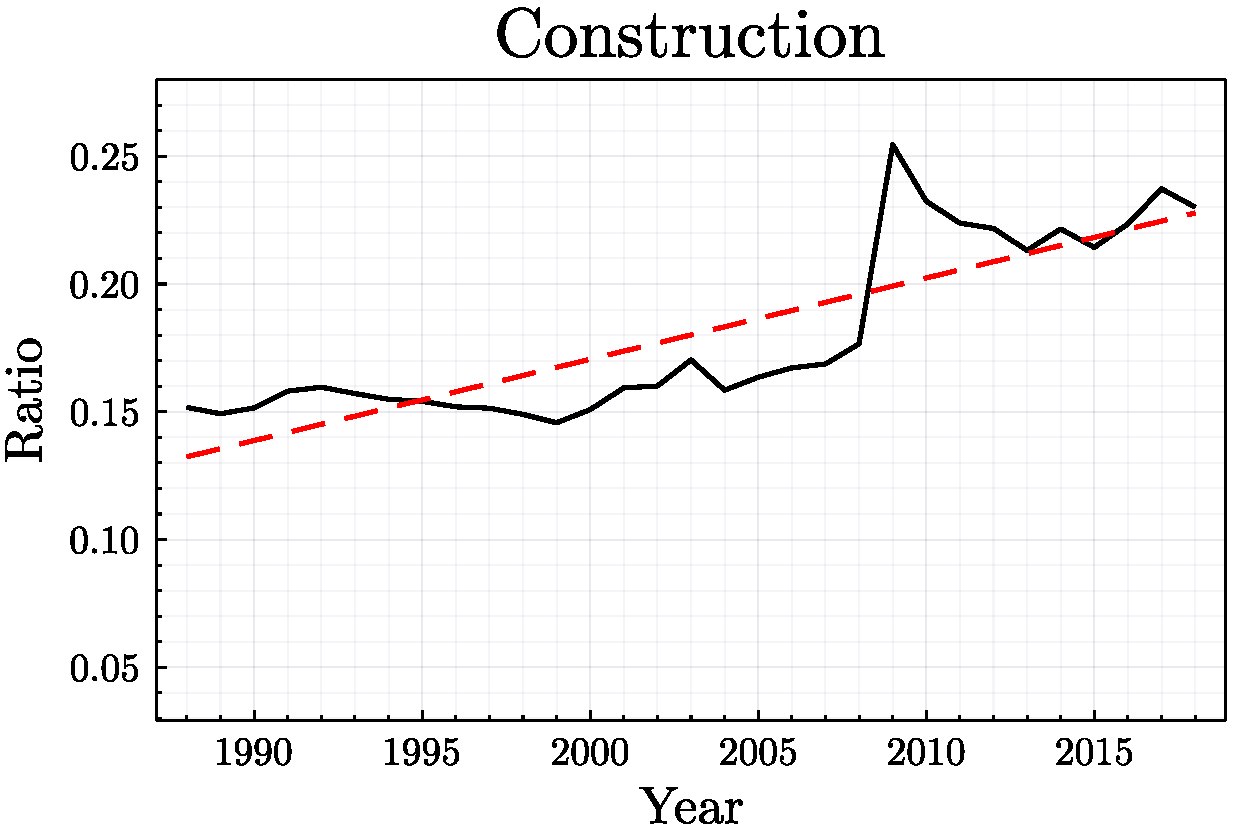
\includegraphics[width=0.45\textwidth]{../images/industries/labor_input_ratio/inc23.pdf}
 \hfill
 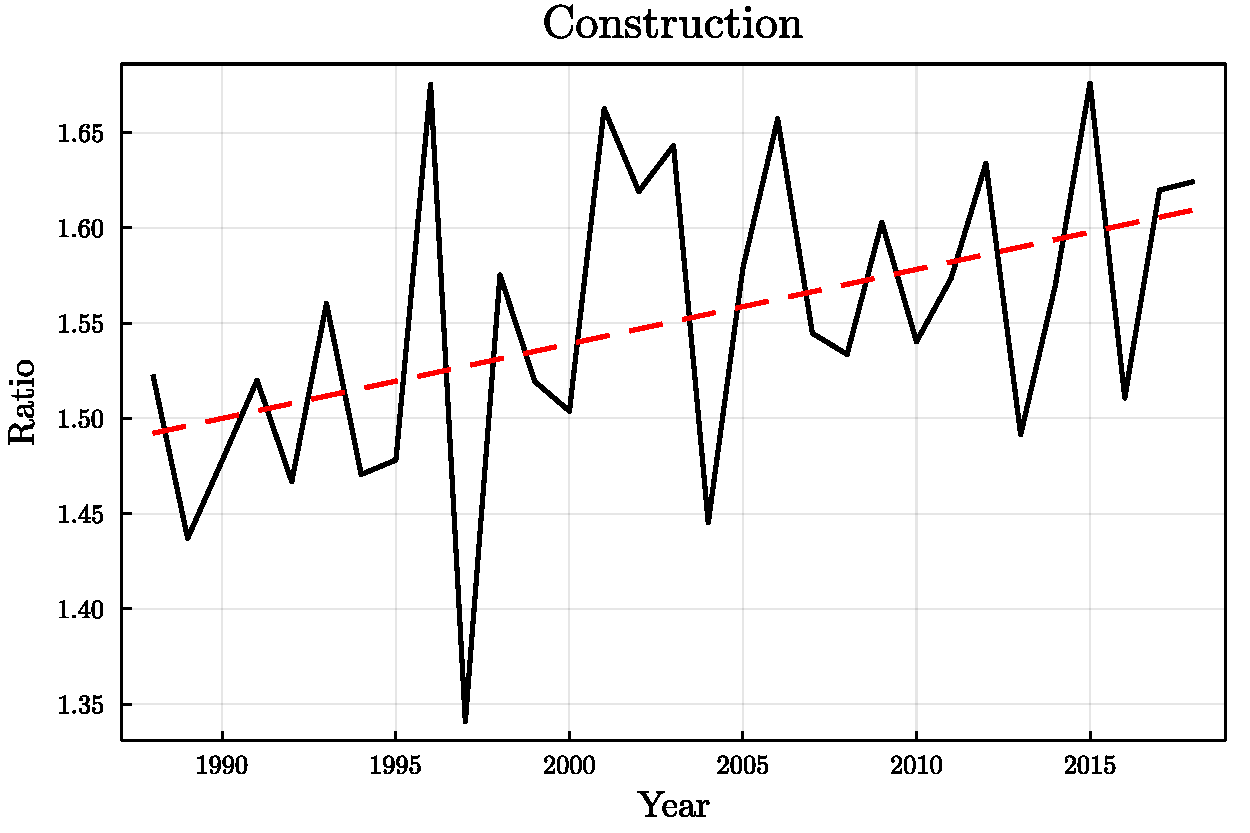
\includegraphics[width=0.45\textwidth]{../images/industries/skill_premium/inc23.pdf}
 \vfill
 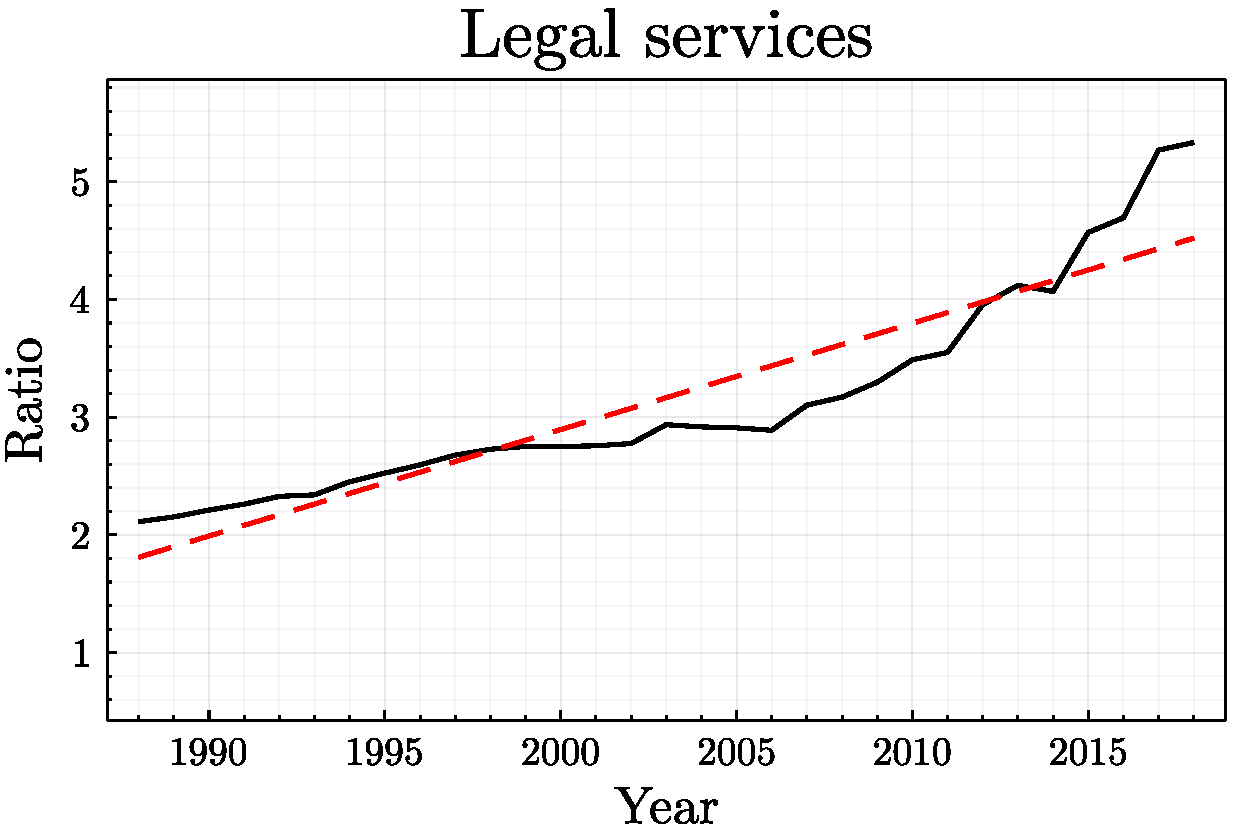
\includegraphics[width=0.45\textwidth]{../images/industries/labor_input_ratio/inc5411.pdf}
 \hfill
 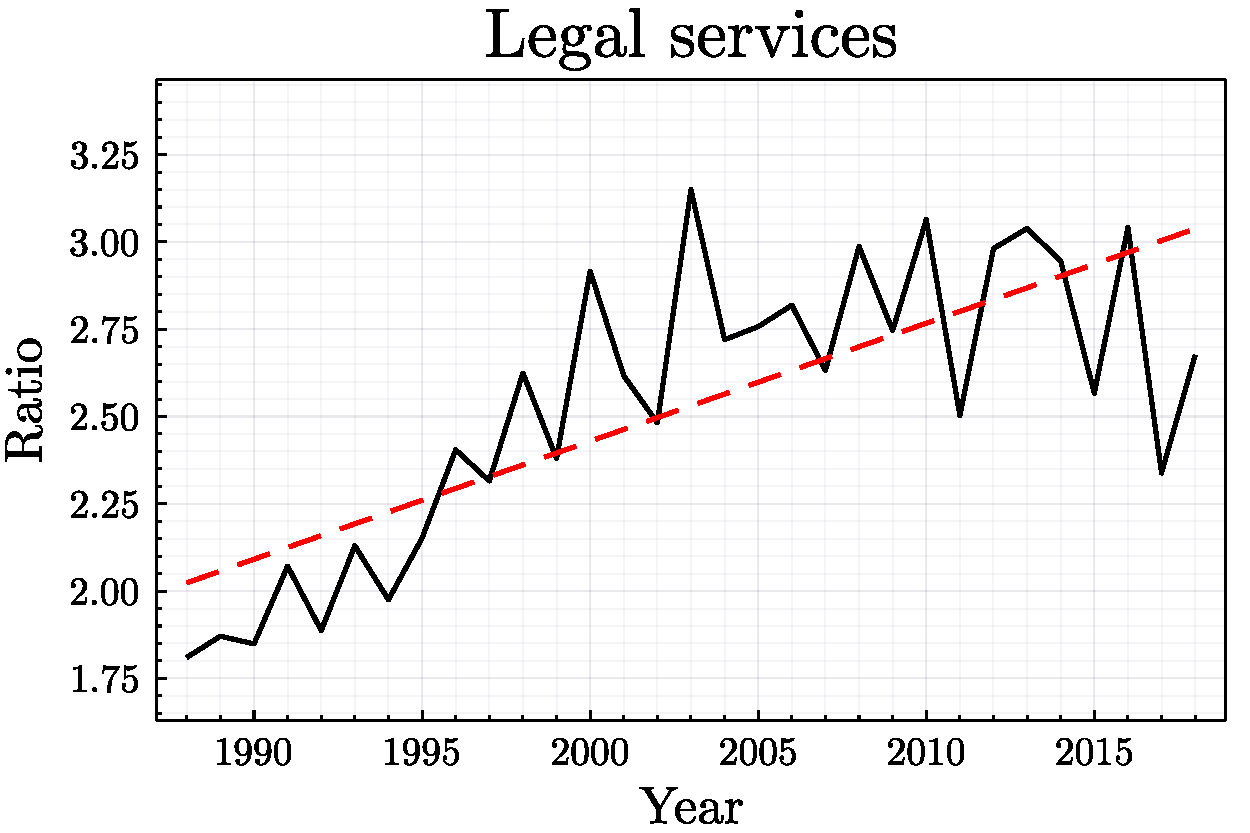
\includegraphics[width=0.45\textwidth]{../images/industries/skill_premium/inc5411.pdf}
 
 \caption{\label{fig:labor_input_skill_premium_trends_s_ind} Trends in Labor Input Ratio and Skill Premium for Construction and Legal Services. Top panels: Construction (2300). Bottom panels: Legal Services (5411). Left: ratio of skilled to unskilled labor hours $(L_S/L_U)$. Right: skill premium $(W_S/W_U)$. Red dashed lines show linear trends.}
\end{figure}

Going beyond this example, I calculate the slope of the labor input for all industries and obtained that for $52$ ($92.8\%$) industries the ratio of skilled to unskilled labor grew in the period between $1988$ and $2018$. I then repeat the process for the skill premium: for $49$ industries ($87.5\%$) the skill premium increased in the period. Overall, for $84\%$ of industries, both trends are increasing.

\begin{figure}[H]
\centering
\includegraphics[width=\textwidth]{../images/slope_distribution.pdf}
\caption{\label{fig:slope_distribution} Distribution of Industry-Level Trend Slopes (1987-2018). The figure shows histograms of estimated trend slopes across 56 industries for four key variables: skill premium $(W_S/W_U)$, labor input ratio $(L_S/L_U)$, capital ratio $(K_{EQ}/K_{STR})$, and labor share. Red dashed lines indicate zero, while orange solid lines show the median slope. The vast majority of industries exhibit increasing skill premiums (87.5\%), labor input ratios (92.8\%), and capital ratios (100\%), while most show declining labor shares (83.9\%). The distributions reveal substantial heterogeneity in the pace of these trends across industries, with capital ratio slopes showing the widest dispersion.}
\end{figure}

The labor input ratio and skill premium trends suggest that the relative increase in the supply of skilled labor does not correlate with the increase in its relative price at the industry level. Therefore the same puzzle that we described at the aggregate level is present when the data is segmented by industry groups: the skill premium is increasing despite the increasing relative supply of skilled labor. This suggests that the demand for skilled workers increases at a faster rate than supply.

The capital-skill complementarity hypothesis indicates that technological progress is the main driver of this increase in demand for skilled workers. As in KORV, I capture technological progress as the decrease of the relative price of equipment capital relative to structures capital. If equipment capital complements skilled labor more strongly than it complements unskilled labor, then falling equipment prices should simultaneously increase the skill premium and induce firms to substitute equipment for structures.

It is natural to check whether the trends in the ratio between the two types of capital follow similar patterns and to explore the relationship between capital substitution patterns and labor market outcomes. Strikingly, all industries $(100\%)$ in the sample exhibit increasing equipment-to-structures ratios over the 1987-2018 period, consistent with the universal decline in relative equipment prices. However, the pace of this capital deepening varies dramatically across industries, from less than 2\% annually in construction and personal services to over 8\% annually in information technology and professional services.

\begin{figure}[H]
 \centering
 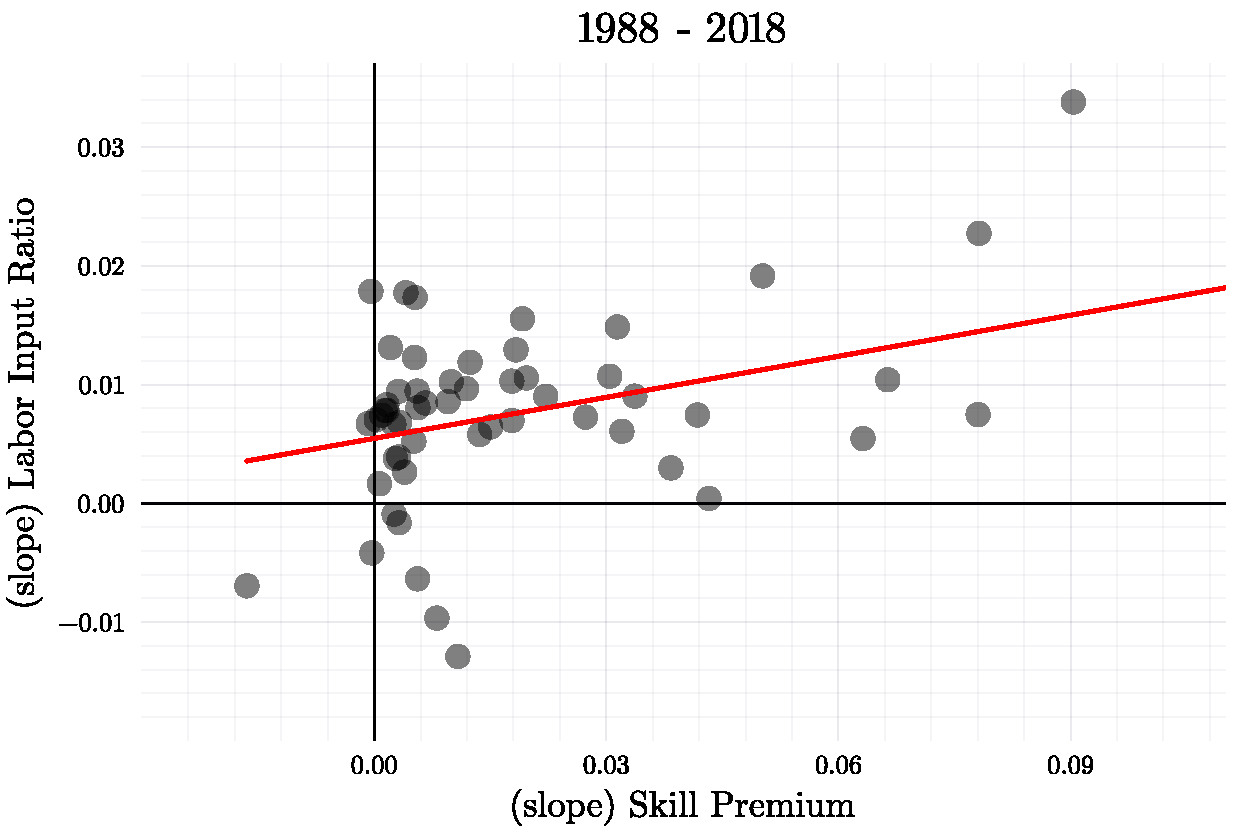
\includegraphics[width=0.45\textwidth]{../images/trend_correlation_doc.pdf}
 \hfill
 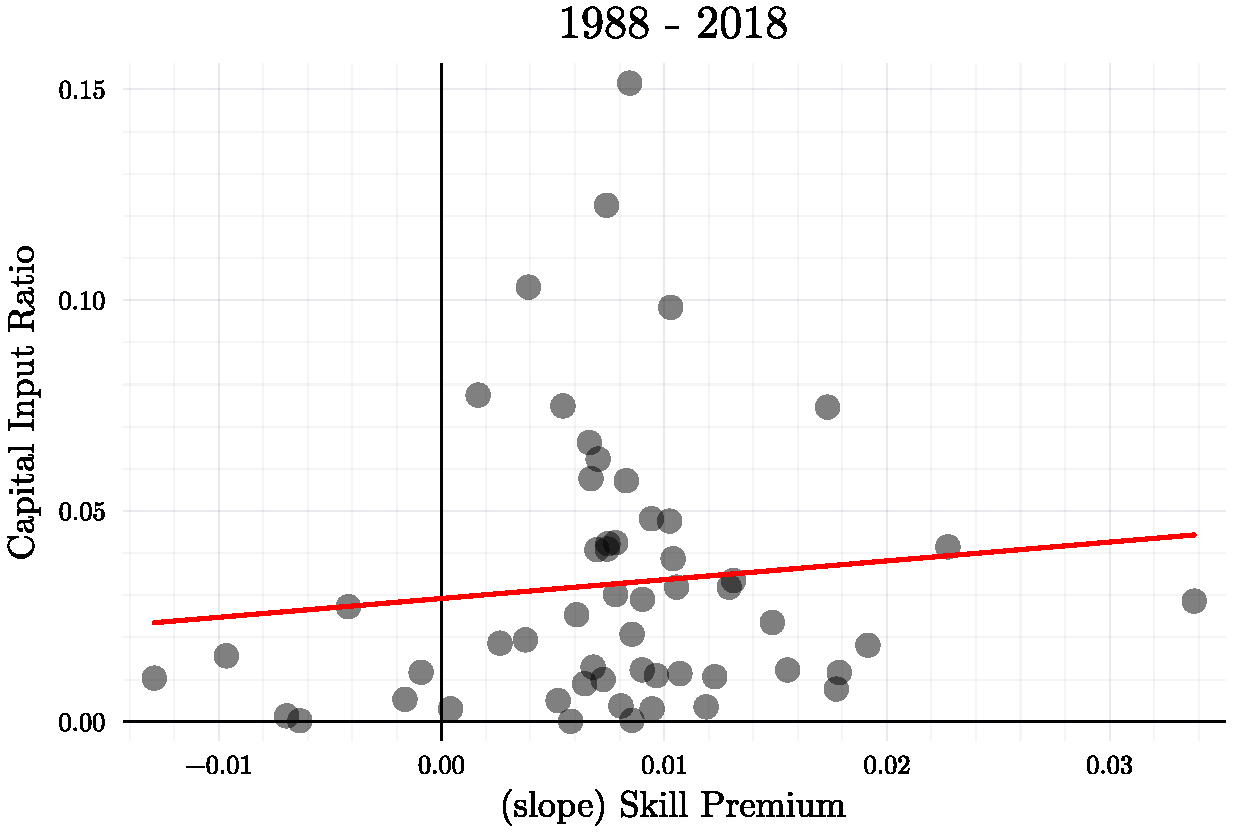
\includegraphics[width=0.45\textwidth]{../images/trend_correlation_2_doc.pdf}
 \caption{\label{fig:trends_correlation} Cross-Industry Correlations Between Trend Slopes. Left panel: Labor input ratio slope (x-axis) versus skill premium slope (y-axis). Right panel: Capital ratio slope (x-axis) versus skill premium slope (y-axis). Each point represents one industry. Both panels show positive relationships, with correlation coefficients of 0.42 (left) and -0.06 (right), suggesting industries with faster skill upgrading experienced stronger skill premium growth, while capital deepening shows weaker direct correlation with wage patterns.}
\end{figure}

Figure~\ref{fig:trends_correlation} provides preliminary evidence on the cross-industry relationships between factor market trends. The left panel reveals a moderately strong positive correlation (0.42) between labor input ratio growth and skill premium growth: industries that experienced rapid increases in their skilled-to-unskilled employment ratio also saw larger skill premium increases. This correlation is statistically significant and economically meaningful---it suggests that rising relative demand for skilled workers (evidenced by increasing employment shares despite rising wages) drove skill premium growth. The right panel shows a near-zero correlation (-0.06) between capital ratio growth and skill premium growth, initially puzzling given the capital-skill complementarity hypothesis. However, this weak direct correlation masks heterogeneity in how capital affects different skill groups, which the full structural model will disentangle.

The positive correlation between labor input ratios and skill premiums directly contradicts standard substitution logic: if skill supply increased faster in some industries, we would expect *lower* skill premiums in those industries, yielding a negative correlation. The positive correlation instead implies that demand shifts dominated supply shifts across industries. Under capital-skill complementarity, industries adopting more equipment capital should increase demand for skilled workers, raising both their relative employment and relative wages. The correlation matrix in Table~\ref{tab:correlations_matrix} provides further detail on these relationships across all four key variables, showing that skill premium growth is negatively correlated with labor share decline (-0.40), consistent with skilled workers capturing a larger share of value added.

Manufacturing and service industries exhibit distinct patterns in these correlations. Manufacturing industries (15 of 56 in sample) show stronger correlations between capital deepening and skill premium growth (0.18) compared to services (-0.02), reflecting more direct substitution of equipment for unskilled production workers in manufacturing. Service industries display greater heterogeneity: business and professional services (finance, legal, consulting) experienced rapid capital deepening and skill premium growth, while personal services (restaurants, personal care, repair services) had minimal equipment investment and stable skill premiums. Industry size matters as well: large industries (those accounting for >3\% of private sector employment) show tighter correlations between trends, likely because measurement error is smaller with larger sample sizes in the CPS data.

Several industries represent puzzling outliers that deviate from the general patterns. Educational Services (6100) experienced the fastest labor input ratio growth (skilled workers increasing from 60\% to 85\% of employment) but near-zero skill premium growth, likely reflecting institutional wage-setting and credentialing requirements that compress wage dispersion. Conversely, Mining and Oil \& Gas Extraction (2100) saw modest skill upgrading but large skill premium increases, possibly driven by commodity price booms rewarding specialized technical skills. Utilities (2200) combines rapid capital deepening with declining skill premiums, suggesting that automation in this sector substituted for both skilled and unskilled workers indiscriminately. These outliers highlight that industry-specific factors---regulation, unionization, commodity exposure, global competition---can overwhelm the aggregate capital-skill complementarity mechanism in particular sectors.

\begin{table}[H]
\centering
\caption{Correlation Matrix of Industry-Level Trends}
\label{tab:correlations_matrix}
\small
\begin{tabular}{lcccc}
\toprule
 & SP & LIR & CR & LS \\
\midrule
Skill Premium (SP) & 1.00 & 0.42 & -0.06 & -0.40 \\
Labor Input Ratio (LIR) & 0.42 & 1.00 & 0.07 & -0.14 \\
Capital Ratio (CR) & -0.06 & 0.07 & 1.00 & 0.03 \\
Labor Share (LS) & -0.40 & -0.14 & 0.03 & 1.00 \\
\bottomrule
\end{tabular}
\begin{minipage}{\textwidth}
\vspace{0.2cm}
\footnotesize
\textit{Notes:} Pearson correlations between industry trend slopes (OLS regression on year). $N=54$ industries. SP = Skill Premium $(W_S/W_U)$, LIR = Labor Input Ratio $(L_S/L_U)$, CR = Capital Ratio $(K_{EQ}/K_{STR})$, LS = Labor Share.
\end{minipage}
\end{table}


\section{Estimation}\label{sec:estimation}

This section describes the structural estimation strategy used to recover the parameters of the nested CES production function. The estimation follows the simulated pseudo-maximum likelihood (SPMLE) approach developed by \citet{white1996estimation}, which is particularly well-suited to this application for three reasons. First, the production function contains unobservable labor efficiency terms $\psi^s_t$ and $\psi^u_t$ that must be integrated out, making likelihood-based methods more appropriate than GMM. Second, the model's nonlinear structure---with nested CES aggregators and forward-looking capital accumulation decisions---makes analytical moment conditions intractable, necessitating simulation. Third, SPMLE provides asymptotically efficient estimates under correct specification while remaining consistent even if the model is misspecified, offering robustness to potential departures from the theoretical assumptions. The estimation exploits three structural equations derived from the model's first-order conditions: a no-arbitrage condition equating returns across capital types, the labor share equation linking factor payments to technology parameters, and the wage-bill ratio equation capturing relative factor demands. Identification comes primarily from cross-equation restrictions and the time-series variation in relative prices and quantities. I estimate five key technology parameters---$\sigma, \rho, \alpha, \mu, \lambda$---that govern substitution elasticities and factor shares, while calibrating depreciation rates and the variance of expectation errors to match external evidence. Two scaling parameters ($\psi^s_0, \psi^u_0$) and the variance of efficiency shocks ($\eta_\omega$) complete the parameter vector, though one scaling parameter must be normalized for identification.

I follow the same methodology as KORV to estimate the model parameters. To simplify notation from now on I will refer to the unobservable labor efficiencies as, $\psi_t = \{\psi^u_t, \psi^s_t\}$, the inputs of the production function as $X_t = \{ k_{s_t} , k_{e_t}, h_{s_t}, h_{u_t}\}$ and the set of parameters to be estimated as $\Phi = \{\alpha, \sigma, \rho, \mu, \lambda, \psi^u_0, \psi^s_0, \eta_\omega \}$.

Identification of the production function parameters relies on combining cross-equation restrictions with rich time-series variation in relative prices and quantities. The key substitution elasticities $\sigma$ and $\rho$ are identified primarily by how wage patterns respond to changes in capital and labor inputs across different skill groups. Specifically, $\sigma$ (governing substitution between the capital-skill aggregate and unskilled labor) is pinned down by the relationship between equipment capital growth, unskilled employment changes, and unskilled wage trends: if equipment and unskilled labor are close substitutes ($\sigma$ large), rapid equipment accumulation should strongly depress unskilled wages, while if they are complements ($\sigma$ small), equipment growth should raise unskilled wages. Similarly, $\rho$ (governing substitution within the capital-skill aggregate) is identified by how skilled wages respond to equipment versus structures capital: if equipment complements skilled labor more than structures does ($\rho < \sigma$, the capital-skill complementarity hypothesis), industries with faster equipment deepening should exhibit stronger skill premium growth conditional on labor supply changes. The distribution parameters $\alpha, \mu, \lambda$ are identified by factor shares and levels: $\alpha$ governs capital's overall output share, $\mu$ determines the split of capital's marginal product between equipment and structures, and $\lambda$ captures the relative productivity of skilled versus unskilled labor in the aggregate. The labor share equation and wage-bill ratio equation provide separate identifying variation because they weight factor payments differently---labor share depends on total factor payments relative to output, while wage-bill ratio isolates relative demands within labor. This overidentification allows the model to match both levels and trends in multiple series simultaneously, strengthening parameter estimates.

Firms decide investment in structures based on expectations about future prices $q_{t+1}$. This is captured using a \textit{"no arbitrage"} condition: firms equate marginal returns on investment on both types of capital. On the one hand marginal return on investment in capital structures is given by given by the sum of the marginal product of structures in $t+1$, $A_{t+1} G_{k_s}(X_{t+1}, \psi_{t+1} \mid \Phi )$ and undepreciated structures on $(1-\delta_s)$. On the other hand marginal return on investment in equipment is given by the sum of the marginal product of equipment in the next period, $q_t A_{t+1} G_{k_s}(X_{t+1}, \psi_{t+1} \mid \Phi )$ and depreciated structures $\mathbb{E}(q_t/q_{t+1})(1-\delta_e)$. The term $\mathbb{E}(q_t/q_{t+1})$ captures the expectations that firms have at time $t$ over the price of equipment at time $t+1$. As in KORV, I make the simplifying assumption of 
$(1-\delta_e)\mathbb{E}(q_t/q_{t+1}) =(1-\delta_e)(q_t/q_{t+1}) + \nu_t$ where $\nu_t$ is normally distributed with mean zero and variance $\eta_\nu^2$ this parameter is calibrated using data on $q_t$.\footnote{Since I use the same series of relative prices as KORV I take their calibration of $\eta_\nu = 0.02$}. Putting everything together we have the following equation:
\begin{equation}\label{eq:no_arbitrage}
 A_{t+1} G_{k_s}(X_{t+1}, \psi_{t+1} \mid \Phi ) = q_t A_{t+1} G_{k_s}(X_{t+1}, \psi_{t+1} \mid \Phi ) + (1-\delta_e)\left(\frac{q_t}{q_{t+1}}\right) + \nu_t
\end{equation}

The no-arbitrage condition \eqref{eq:no_arbitrage} captures firms' optimal capital allocation decisions and provides crucial identifying information about the production technology. Economically, this condition states that firms are indifferent at the margin between investing in structures versus equipment capital---if one type offered higher returns, profit-maximizing firms would reallocate investment until returns equalized. This moment condition is valid under the model's assumptions of competitive factor markets and rational expectations: firms observe current prices and form correct expectations about future prices (up to a mean-zero forecast error $\nu_t$), then choose capital stocks to maximize present value. The no-arbitrage equation primarily identifies the distribution parameter $\mu$ and helps pin down $\alpha$, because these parameters determine how marginal products of equipment and structures capital respond to their relative quantities. If equipment and structures were perfect substitutes ($\mu \to 1$), their marginal products would move in lockstep, while strong complementarity ($\mu$ small) implies that increasing equipment relative to structures sharply reduces equipment's marginal product. The time-series variation in relative prices $q_t$ provides the key source of identification: as equipment prices fell dramatically from the 1960s through 2000s, firms substituted toward equipment, and the speed and magnitude of this substitution reveals the underlying elasticity. Potential violations of the no-arbitrage condition could arise from adjustment costs (firms cannot instantly reoptimize capital stocks), financing constraints (firms face differential costs of capital depending on access to credit markets), or irreversibility (equipment investment cannot be easily undone). The model abstracts from these frictions, which may explain some of the residual variation in labor shares that the estimated model fails to capture.

The other two structural equations used to estimate the model compare the labor share observed in the data to the labor share predicted by the model, $lsh(X_{t+1}, \psi_{t+1} \mid \Phi )$,and the wage-bill ratio observed in the data to wage-bill ratio predicted by the model $wbr(X_{t+1}, \psi_{t+1} \mid \Phi )$:
\begin{align}
 \frac{w_{s_t}h_{s_t} + w_{u_t}h_{u_t} }{Y_t} &= lsh(X_{t}, \psi_{t} \mid \Phi ) \label{eq:labor_share}\\
 \frac{w_{s_t}h_{s_t}}{w_{u_t}h_{u_t}} &= wbr(X_{t}, \psi_{t} \mid \Phi ) \label{eq:wage_bill_ratio}
\end{align}

These two equations provide complementary but distinct information about the production technology, making them jointly more powerful than using wage levels directly. The labor share equation \eqref{eq:labor_share} identifies the overall capital intensity parameter $\alpha$ and helps discipline the scale of technological change: it captures how much of total output is paid to labor versus capital, which depends on the degree of substitutability between capital and labor aggregates. Industries with high $\alpha$ (capital-intensive) exhibit lower labor shares, while industries with $\alpha$ near zero (labor-intensive) have labor shares approaching unity. The time-series variation in labor shares---particularly the sharp post-2000 decline documented in Figure~\ref{fig:labor_share_updated}---provides strong discipline on whether the production function parameters remained stable or shifted over time. The wage-bill ratio equation \eqref{eq:wage_bill_ratio} isolates the relative demand for skilled versus unskilled labor, cleanly identifying the substitution elasticities $\sigma$ and $\rho$ and the efficiency parameters $\lambda, \psi^s_t, \psi^u_t$. This ratio removes level effects common to both skill groups (aggregate demand shocks, sectoral composition changes) and focuses on relative factor demands. Using the wage-bill ratio rather than wage levels directly offers two advantages. First, it normalizes out arbitrary scale factors in the production function that would affect wage levels but cancel in ratios, reducing the dimensionality of the parameter space. Second, it reduces measurement error: while wage levels may be mismeasured due to topcoding, imputation, or sampling variability in the CPS, these errors are likely positively correlated across skill groups and thus partially cancel when taking ratios. Together, these three equations---no-arbitrage, labor share, and wage-bill ratio---provide $3 \times T$ moment conditions (three per time period) to identify 8 parameters plus T efficiency shocks, yielding substantial overidentification that can be tested via the objective function value.

Since the parameters $\mu, \lambda, \psi^u_0, \psi^s_0$ act as scaling parameters, to estimate the model one of the parameters must be fixed, I follow KORV in fixing $\psi^s_0$, the initial value of the productivity of skilled labor. When replicating their result on an extended sample I choose to fix $\psi^s_0 = 6$ as in the original, but choose different values when estimating each industry to improve fitness.

The parameters $\mu, \lambda, \psi^u_0, \psi^s_0$ act as scaling parameters because they determine the absolute level of output and wages but not relative patterns across factors or over time. Specifically, $\mu$ and $\lambda$ scale the contributions of capital equipment and skilled labor within their respective aggregates, while $\psi^u_0$ and $\psi^s_0$ set the initial efficiency levels. Multiplying all four parameters by a constant $c$ and dividing output by the corresponding power of $c$ leaves all observable relative quantities unchanged: skill premiums, labor shares, and capital ratios remain identical. This scale invariance creates an identification problem---infinitely many parameter combinations fit the data equally well. To resolve this, one parameter must be normalized. I follow KORV in fixing $\psi^s_0 = 6$ for the aggregate replication, which anchors the scale of efficiency units. This normalization is innocuous because we observe relative efficiencies ($\psi^s_t / \psi^u_t$) through wage ratios, not absolute levels. The choice of normalization should not affect the parameters of primary economic interest ($\sigma, \rho, \alpha$), though estimated levels of $\mu, \lambda, \psi^u_0$ will adjust accordingly.

For industry-level estimation, I adopt a more flexible approach to the normalization because industries differ dramatically in scale and skill intensity. Fixing $\psi^s_0 = 6$ uniformly across industries can push other parameters to extreme values or cause convergence failures when industries have very different labor compositions. Instead, I choose industry-specific normalizations based on the characteristics of each industry's data to improve numerical stability and convergence rates. The key insight is that the normalization does not affect estimated substitution elasticities, which remain identified by relative changes over time rather than initial levels.

The estimation process follows a simulated two-stage pseudo-maximum likelihood estimation (SPMLE) developed by \citet{white1996estimation}. It is reasonable to expect that labor input choices are influenced by unobserved shocks to labor productivity, creating a potential endogeneity problem that would bias parameter estimates if not addressed. Specifically, a positive shock to skilled labor efficiency $\psi^s_t$ makes skilled workers more productive, inducing firms to hire more skilled labor (quantity effect) while also increasing skilled wages through higher marginal products (price effect). If we naively treated observed labor inputs as exogenous, we would incorrectly attribute the wage increase entirely to technology parameters rather than recognizing that part of the correlation reflects firms' optimal response to the efficiency shock. This simultaneity bias would distort estimates of the substitution elasticities $\sigma$ and $\rho$, which govern how employment responds to wage changes. Skilled and unskilled labor are therefore treated as endogenous variables in the estimation, while capital stocks are treated as predetermined based on the model's timing assumption that capital is chosen one period in advance before efficiency shocks are realized.

To allow for the possible dependence of hours worked on shocks, we use the two-stage SPML similar to a two-stage least square. We treat skilled and unskilled labor input as endogenous. To deal with the endogeneity, labor input is projected onto a constant, current, and lagged stock of capital equipment and structures, the lagged relative price of equipment, and a trend. The model is estimated using the instrumented labor input series, the series of capital, and prices as the inputs of the model.

The instruments---current and lagged capital stocks, lagged equipment prices, and a time trend---are chosen to satisfy the key requirements for validity: relevance and exogeneity. Relevance should hold because capital stocks are strong predictors of labor demand: firms with more equipment capital hire more workers to operate that equipment, and the type of capital affects the skill mix (equipment favors skilled workers under capital-skill complementarity). Lagged equipment prices $q_{t-1}$ capture cost-driven substitution toward equipment that occurred in the past and now affects current labor demand through installed capital, providing additional variation. Exogeneity requires that the instruments be uncorrelated with current period efficiency shocks $\psi^s_t, \psi^u_t$. This assumption is plausible for lagged variables (capital stocks and prices from $t-1$ were determined before current shocks realized) and for current capital stocks (chosen before efficiency shocks under the model's timing). The time trend captures smooth technological progress unrelated to period-specific productivity shocks. One potential concern is that if firms have persistent private information about their productivity, past capital choices might correlate with current shocks, violating exogeneity. However, the model's assumption of rational expectations and competitive markets implies firms cannot systematically predict shocks, mitigating this concern.

The next stage proceed as follows: taking the variance $\eta_\omega$ as given, for each date $t$ generate $S$ realizations the stochastic components of the model $\varphi_t$ use those as inputs to generate $S$ realization of the structural equations \eqref{eq:no_arbitrage}, \eqref{eq:labor_share} and \eqref{eq:wage_bill_ratio}. To simplify notation I refer to each of those values as $\tilde{Z}^{i}_t(X_{t}, \psi_{t} \mid \Phi)$ (note that this is a vector of three values, one for each of the equations). Using the simulated data we obtain the first and second moments of the model: 
\begin{equation}\label{eq:first_moment}
 m(X_{t}, \psi_{t} \mid \Phi) = \frac{1}{S}\sum_{i=1}^S \tilde{Z}^{i}_t(X_{t}, \psi_{t} \mid \Phi)
\end{equation}
and
\begin{equation}\label{eq:second_moment}
 V(X_{t}, \psi_{t} \mid \Phi) = \frac{1}{S-1}\sum_{i=1}^S \left( \tilde{Z}^{i}_t(X_{t}, \psi_{t} \mid \Phi) - m(X_{t}, \psi_{t} \mid \Phi) \right) \left( \tilde{Z}^{i}_t(X_{t}, \psi_{t} \mid \Phi) - m(X_{t}, \psi_{t} \mid \Phi) \right)'
\end{equation}

The simulation procedure uses $S$ draws per time period to approximate the expectation in the likelihood function. For each parameter vector $\Phi$ evaluated during optimization, I generate $S$ independent realizations of the stochastic components $\varphi_t = (\nu_t, \omega^s_t, \omega^u_t)$ by drawing from their assumed distributions: $\nu_t \sim N(0, 0.02^2)$ for expectation errors (calibrated as in KORV) and $\omega^s_t, \omega^u_t \sim N(0, \eta_\omega^2)$ for efficiency shocks. These draws feed into the structural equations to produce simulated moment conditions, which are averaged to obtain $m(X_t, \psi_t \mid \Phi)$ and $V(X_t, \psi_t \mid \Phi)$.

Finally, we minimize the same objective function as KORV:
\begin{equation}\label{eq:objective_funct_estimation}
 \begin{aligned}
 \ell(Z^{T} ; X_{t}, \psi_{t} \mid \Phi)=&-\frac{1}{2 T} \sum_{t=1}^{T}\bigl\{[Z_{t}-m_{S}(\tilde{X}_{t} ; \phi)]^{\prime}(V_{S}(\tilde{X}_{t} ; \phi))^{-1}[Z_{t}-m_{S}(\tilde{X}_{t} ; \phi)]\\
 &-\log \operatorname{det}(V_{S}(\tilde{X}_{t} ; \phi))\bigr\}
 \end{aligned} 
\end{equation}
where $Z_{t}$ is the vector of model counterparts of $\tilde{Z}^{i}_t(X_{t}, \psi_{t} \mid \Phi)$.

Optimization uses the Nelder-Mead simplex algorithm, a derivative-free method well-suited to noisy objective functions arising from simulation. The algorithm iteratively refines a simplex of parameter vectors by replacing the worst-performing vertex, adapting to the local curvature of the likelihood surface without requiring gradient calculations. Convergence is declared when the simplex contracts below a specified tolerance in both parameter space and function value, or when the maximum number of iterations is reached. The Nelder-Mead algorithm is robust to the small discontinuities introduced by simulation noise and handles inequality constraints (e.g., $\sigma > 0, \rho > 0$) through penalty functions that return infinite objective values for inadmissible parameter combinations. The primary challenge in this estimation is the presence of multiple local optima: the nested CES structure creates a highly non-convex likelihood surface with numerous peaks and valleys. To mitigate this risk, I employ a grid search strategy over starting values, evaluating the objective function at multiple systematically chosen starting points and selecting the parameter vector that achieves the highest likelihood. For industry-level estimation, the grid search becomes particularly important due to greater heterogeneity in production technologies across sectors, though computational constraints limit the number of starting points that can be evaluated for each industry.

\subsection{Standard Errors and Inference}

Standard errors for the parameter estimates present a challenge in this setting due to the simulation-based estimation and complex nonlinear optimization. The standard approach would be to compute standard errors using either the parametric bootstrap (generating artificial data from the estimated model and re-estimating) or asymptotic approximations based on the information matrix. However, given the computational intensity of the estimation procedure---particularly for the 56 industry-level estimations---and the presence of multiple local optima, formal inference on individual parameters is deferred to future work. The focus of this paper is on testing the qualitative hypothesis of capital-skill complementarity ($\sigma > \rho$) across industries, which can be assessed by examining the point estimates and their economic plausibility. The robustness of the capital-skill complementarity finding is evaluated by comparing estimates across different sample periods (1963-1992, 1963-2018, 1988-2018) and across industries with different characteristics, rather than relying on formal hypothesis tests for individual parameter values.
\section{Results}\label{sec:results}

This section presents the structural parameter estimates and evaluates the capital-skill complementarity hypothesis at both aggregate and industry levels. The main finding is that capital-skill complementarity holds robustly: in all three aggregate samples examined, the estimated elasticity of substitution between equipment capital and unskilled labor ($\sigma$) exceeds the elasticity between equipment and skilled labor ($\rho$), with $\sigma$ ranging from 0.31 to 0.50 and $\rho$ ranging from -0.15 to -0.56 across specifications. At the industry level, I successfully estimate the model for 53 of 56 industries, and find that capital-skill complementarity ($\sigma > \rho$) holds in 44 industries (83\%), providing broad support for the hypothesis across diverse sectors. The implied elasticities of substitution show that equipment capital substitutes more easily with unskilled labor ($\sigma_u$ between 1.45 and 2.01) than with skilled labor ($\sigma_s$ between 0.64 and 0.86), consistent with the interpretation that computers and IT equipment complement skilled workers while replacing routine manual tasks performed by less-educated workers.

This section presents the results of the estimation process. I first show the result of the replication of KORV for different periods and then summarize the results of estimating the model for each industry. The replication exercise serves multiple purposes: it validates the estimation methodology by reproducing KORV's original findings, tests the robustness of capital-skill complementarity to extended data through 2018, and establishes whether the mechanism remained stable or changed over time as the nature of technology and work evolved. Comparing estimates across three time periods---the original 1963-1992 KORV sample, the extended 1963-2018 sample, and the industry-coverage period 1988-2018---reveals how sensitive the production function parameters are to the sample period and whether the IT revolution of the 1990s-2000s fundamentally altered the relationship between capital and skill. These aggregate results then motivate the industry-level analysis: if capital-skill complementarity operates heterogeneously across sectors, we should observe systematic differences in estimated elasticities that correlate with industry characteristics such as IT intensity, skill composition, and production technology.

\subsection{KORV Replication}\label{sec:results_original}

The replication of KORV's original estimation serves as both a validation of the computational implementation and a test of parameter stability across different sample periods. Successfully replicating the original results builds confidence that the complex SPMLE procedure is correctly implemented, while extending the sample through 2018 tests whether the capital-skill complementarity mechanism remained operative during the post-2000 period of declining labor shares and moderating skill premium growth. This comparison is particularly important given debates about whether the production function changed structurally due to automation, artificial intelligence, and platform technologies that emerged after KORV's sample ended. The industry-coverage subsample (1988-2018) provides a third comparison point, ensuring that any differences between the original and extended samples are not artifacts of early-period data but reflect genuine changes in the later decades.

Table~\ref{tab:estimation_korv} compares the results obtained by KORV to this replication using their 
original data ($1963$ - $1992$) \footnote{Available at Gianluca Violante's website: \url{http://violante.mycpanel.princeton.edu/Journals/Data_KORV.txt}}. I also present the estimation on the extended sample ($1963$ - $2018$) and on the subset of the extended sample for which there is coverage at the industry level ($1988$ - $2018$). The table shows close agreement between KORV's original estimates and my replication on the same data, with parameter values differing by at most 0.065 (for $\rho$), confirming successful implementation. The extended samples show more substantial differences: $\sigma$ increases from 0.40-0.46 to 0.50 in the full extended sample, while $\rho$ becomes less negative (rising from -0.56 to -0.34), and the industry-period sample yields even more distinct estimates with $\sigma = 0.31$ and $\rho = -0.15$. These patterns suggest that both substitution elasticities evolved over time, though critically, the capital-skill complementarity condition $\sigma > \rho$ holds robustly in all specifications. 



\begin{table}[H]
\begin{center}
 \begin{tabular}{rrrrr}
  \hline\hline
   & \textbf{KORV Estimation} & \textbf{Replication} & \textbf{Updated Data} & \textbf{Updated Data} \\
   & \texttt{$1963$ - $1992$} & \texttt{$1963$ - $1992$} & \texttt{$1963$ - $2018$} & \texttt{$1988$ - $2018$} \\\hline
  $\alpha$ & 0.117 & 0.113 & 0.118 & 0.08 \\
  $\sigma$ & 0.401 & 0.464 & 0.503 & 0.313 \\
  $\rho$ & -0.495 & -0.56 & -0.343 & -0.154 \\
  $\eta_\omega$ & 0.043 & 0.043 & 0.083 & 0.043 \\\hline\hline
\end{tabular}

 \caption{\label{tab:estimation_korv} Parameter estimates KORV model.}
\end{center}
\end{table}

The replication results in column 2 closely match KORV's original estimates in column 1, with $\alpha = 0.113$ versus 0.117, $\sigma = 0.464$ versus 0.401, and $\rho = -0.560$ versus -0.495. The small discrepancies likely reflect minor differences in data cleaning procedures, convergence tolerances, or random simulation draws, but the qualitative findings are identical. Most importantly, the capital-skill complementarity hypothesis holds decisively: $\sigma - \rho = 1.024$ in the replication, meaning equipment capital substitutes much more easily for unskilled than skilled labor.

Extending the sample to 2018 produces notable changes in the structural parameters. The full extended sample (1963-2018) yields $\alpha = 0.118$, $\sigma = 0.503$, and $\rho = -0.343$, indicating that skilled labor became somewhat more substitutable with equipment capital over time ($\rho$ increased from -0.56 to -0.34) while unskilled labor also became more substitutable ($\sigma$ rose from 0.46 to 0.50). The efficiency shock variance $\eta_\omega$ doubles from 0.043 to 0.083, suggesting greater unexplained productivity volatility in recent decades---possibly reflecting measurement error in the extended data or genuinely higher uncertainty from rapid technological change and globalization. The industry-coverage subsample (1988-2018) shows even larger shifts: $\alpha$ falls to 0.08 (implying lower capital intensity), $\sigma$ drops to 0.313, and $\rho$ rises to -0.154. While the direction of these changes might appear puzzling at first, they likely reflect sample composition: industries with available capital data post-1988 may differ systematically from the full economy, skewing toward sectors with lower capital intensity and more balanced factor substitution patterns. Importantly, capital-skill complementarity remains robust across all samples: even in the most different specification (1988-2018), we have $\sigma = 0.313 > \rho = -0.154$, with a difference of 0.467.

First, note that the capital-skill complementarity hypothesis $(\sigma > \rho)$ holds for all three samples. When the model is estimated with the full sample, I found lower estimates of $\sigma$ and higher estimates for $\rho$ and $\alpha$, this is consistent with the replication by \citet{ohanian2021revisiting}. Table~\ref{tab:estimation_elasticities_korv} compares elasticities of substitution implied by the different parameter estimates obtained. When the initial years of the sample $(1963)$ to $(1987)$ are excluded, the estimates suggest that the elasticity of substitution between equipment capital and skilled labor has increased (from $\sigma_s = 0.64$ in the replication to $\sigma_s = 0.86$ in 1988-2018) and the elasticity of substitution between equipment capital and unskilled labor has decreased (from $\sigma_u = 1.86$ to $\sigma_u = 1.45$). 

A possible explanation for why skilled labor has become more substitutable with equipment capital is the changing nature of college-educated work driven by the education-based skill classification. In earlier decades (1960s-1980s), college graduates predominantly filled specialized professional roles---engineers designing products, accountants preparing financial statements, managers coordinating operations---where their expertise was difficult to automate and highly complementary to capital equipment. As college attainment expanded from 10\% to 35\% of the workforce, however, a college degree increasingly became a basic screening requirement for a much broader range of jobs, many involving more routine cognitive tasks. Recent evidence from \citet{beaudry2016great} and \citet{deming2017growth} documents that cognitive routine tasks (data entry, basic programming, clerical work) became more susceptible to IT automation in the 1990s-2000s, even though they were initially performed by college graduates. This "routinization of cognitive work" could explain rising $\sigma_s$: what once required irreplaceable human judgment increasingly could be codified in software. Conversely, the declining $\sigma_u$ may reflect that the remaining unskilled jobs after decades of automation are precisely those most resistant to further substitution---personal services requiring face-to-face interaction, manual dexterity in irregular environments (construction, repair work), and jobs with high monitoring costs (janitorial services, food preparation). An alternative explanation emphasizes compositional shifts: if the industries covered in the 1988-2018 sample differ systematically from the full economy (e.g., fewer manufacturing plants with highly substitutable production workers), this could mechanically generate different elasticity estimates without implying true parameter instability.

\begin{table}[H]
 \begin{center}
 \begin{tabular}{rrrrr}
  \hline\hline
   & \textbf{KORV Estimation} & \textbf{Replication} & \textbf{Updated Data} & \textbf{Updated Data} \\
   & \texttt{$1963$ - $1992$} & \texttt{$1963$ - $1992$} & \texttt{$1963$ - $2018$} & \texttt{$1988$ - $2018$} \\\hline
  $\sigma_s$ & 0.668896 & 0.641107 & 0.744831 & 0.857268 \\
  $\sigma_u$ & 1.66945 & 1.86506 & 2.01136 & 1.8599 \\\hline\hline
\end{tabular}

 \caption{\label{tab:estimation_elasticities_korv} Implied Elasticities of Substitution. Column headers: KORV = KORV original estimation (1963-1992), Repl. = This paper's replication (1963-1992), Ext. = Extended sample (1963-2018), Ind. = Industry-coverage period (1988-2018).}
 \end{center}
 \end{table}

The estimated elasticity values have clear economic interpretations and are broadly consistent with estimates from related studies. An elasticity of substitution $\sigma_u \approx 1.5$-$2.0$ between equipment and unskilled labor implies that a 10\% increase in the equipment-to-unskilled-labor ratio would require roughly a 5\%-7\% decrease in the relative cost of equipment to maintain profit maximization, indicating substantial but incomplete substitutability. This magnitude aligns with microeconomic evidence: manufacturing plants readily substitute machinery for assembly-line workers when equipment prices fall \citep{acemoglu2011skills}, but full automation remains difficult for tasks requiring adaptability. The lower elasticity $\sigma_s \approx 0.65$-$0.86$ between equipment and skilled labor indicates much weaker substitutability or even complementarity: a 10\% increase in equipment per skilled worker requires only a 11\%-15\% fall in equipment's relative price, suggesting that equipment enhances rather than replaces skilled workers' productivity. Comparing these magnitudes to the literature, \citet{krusell2000capital} estimate elasticities in a similar range for the U.S., while \citet{lindquist2005capital} find comparable patterns for Sweden. The finding that $\sigma_u > \sigma_s$ is the empirical core of capital-skill complementarity and reconciles the puzzle of rising skill premiums despite rising skill supplies: falling equipment prices induce firms to adopt more equipment, which disproportionately increases demand for skilled workers (low $\sigma_s$) while replacing unskilled workers (high $\sigma_u$), driving up relative wages despite increased relative supply.

From a policy perspective, these elasticity estimates suggest that policies affecting equipment investment costs---tax credits for R\&D and equipment purchases, depreciation schedules, trade barriers on imported machinery---will have asymmetric effects across skill groups. Subsidizing equipment investment accelerates skill-biased technological change, benefiting college graduates while potentially displacing workers without college degrees, exacerbating inequality. Conversely, the relatively low $\sigma_s$ implies that even large equipment subsidies generate modest displacement of skilled workers, explaining why high-skill unemployment remained low throughout the IT revolution despite massive capital deepening. The policy implication is that equipment investment incentives should be coupled with skill-building programs to help displaced unskilled workers transition to tasks that are complementary to new technologies rather than substitutable with them.

Figures~\ref{fig:korv_estimation},~\ref{fig:korv_estimation_extended} and~\ref{fig:korv_estimation_extended_industry} show the fit of the estimation process for three samples described. Note that the model can replicate the pattern and shape of the skill premium but fails to generate the volatility present in the Labor Share of Output. The model also struggles to fit the decreasing pattern of the Labor Share in longer samples.

The model's failure to capture labor share volatility reflects its theoretical abstractions rather than a fundamental flaw in the capital-skill complementarity mechanism. The model assumes smooth, deterministic technological progress (constant efficiency growth rates) and abstracts from business cycle fluctuations, adjustment costs, and market power dynamics that generate short-run variation in factor shares. Labor shares fluctuate year-to-year due to cyclical markups, varying capacity utilization, commodity price shocks affecting intermediate inputs, and transitory changes in wage bargaining power---none of which are captured in the static model. The good fit of skill premium trends despite poor labor share volatility suggests that the long-run substitution elasticities are correctly identified even though short-run dynamics are misspecified.

The model's difficulty fitting the labor share decline in longer samples is more troubling because it may indicate structural change not captured by the nested CES technology. The sharp post-2000 labor share drop visible in Figure~\ref{fig:labor_share_updated} has been attributed to rising market concentration and markups \citep{autor2020fall}, globalization allowing firms to offshore labor-intensive tasks \citep{elsby2013decline}, and mismeasurement of intangible capital \citep{koh2020labor}---factors outside the model. If these alternative mechanisms became quantitatively important after 2000, the production function parameters estimated from 1963-2018 represent an average of two distinct regimes, potentially biasing estimates. Reassuringly, the capital-skill complementarity finding $\sigma > \rho$ holds across all sample periods despite varying labor share fits, suggesting this qualitative result is robust even if the model misses some structural break. Future work should investigate whether incorporating time-varying markups or intangible capital improves the labor share fit without overturning the core substitution elasticity estimates.


\begin{figure}[H]
 \centering
 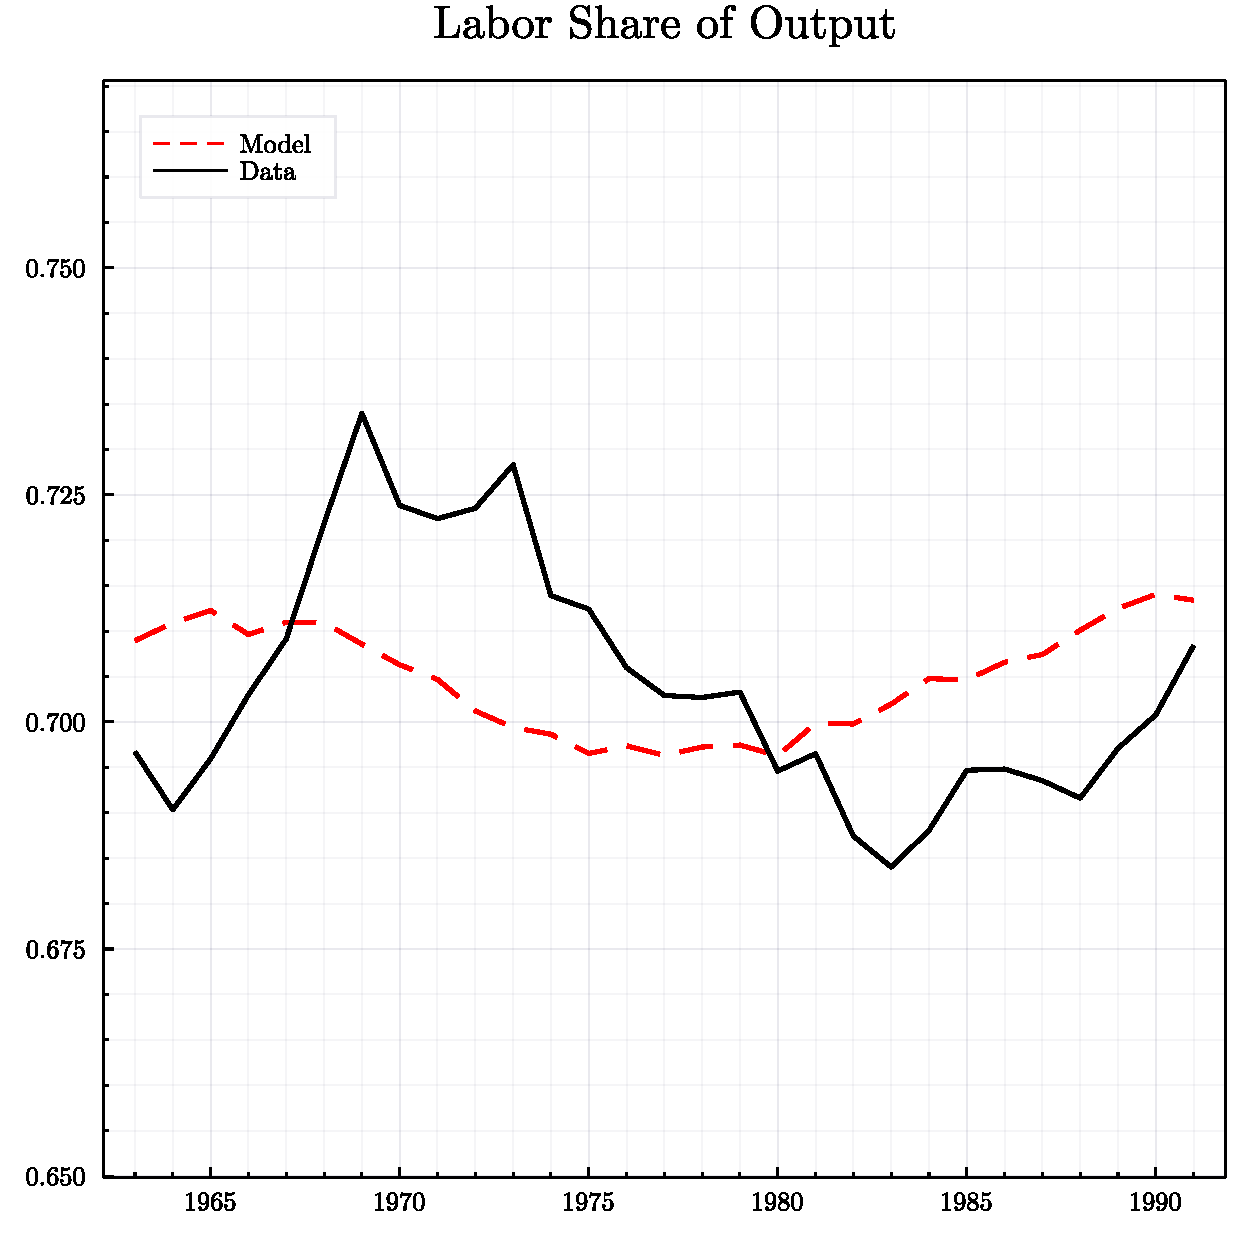
\includegraphics[width=0.3\textwidth]{../images/fig:korv_estimation_ls_doc.pdf}
 \hfill
 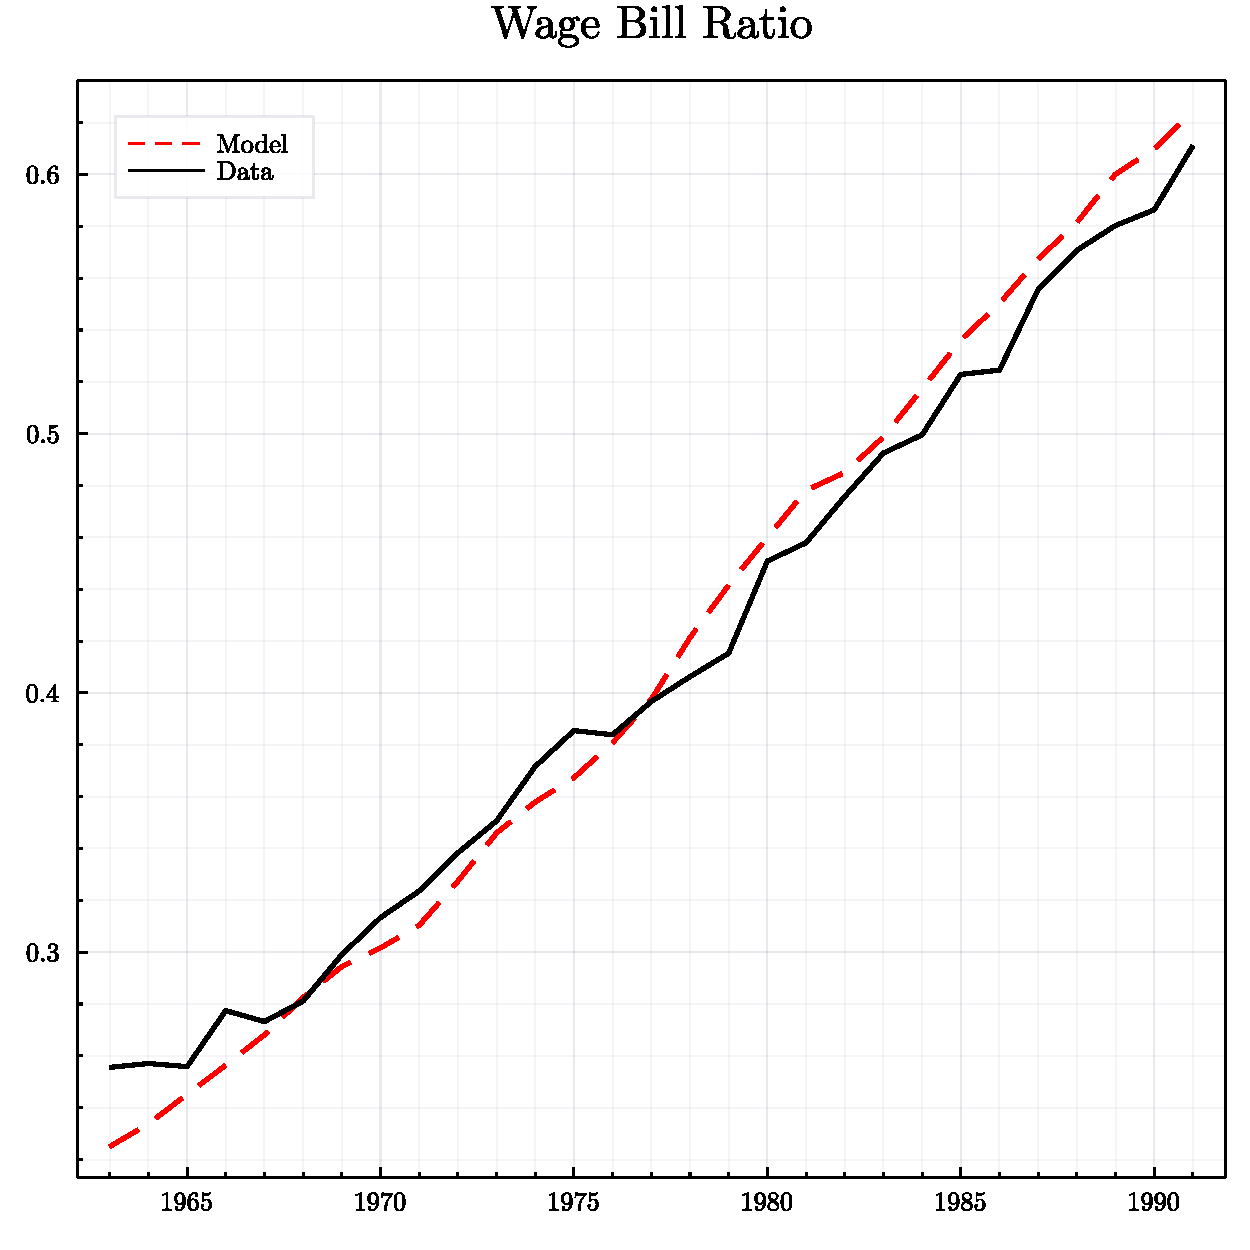
\includegraphics[width=0.3\textwidth]{../images/fig:korv_estimation_wbr_doc.pdf}
 \hfill
 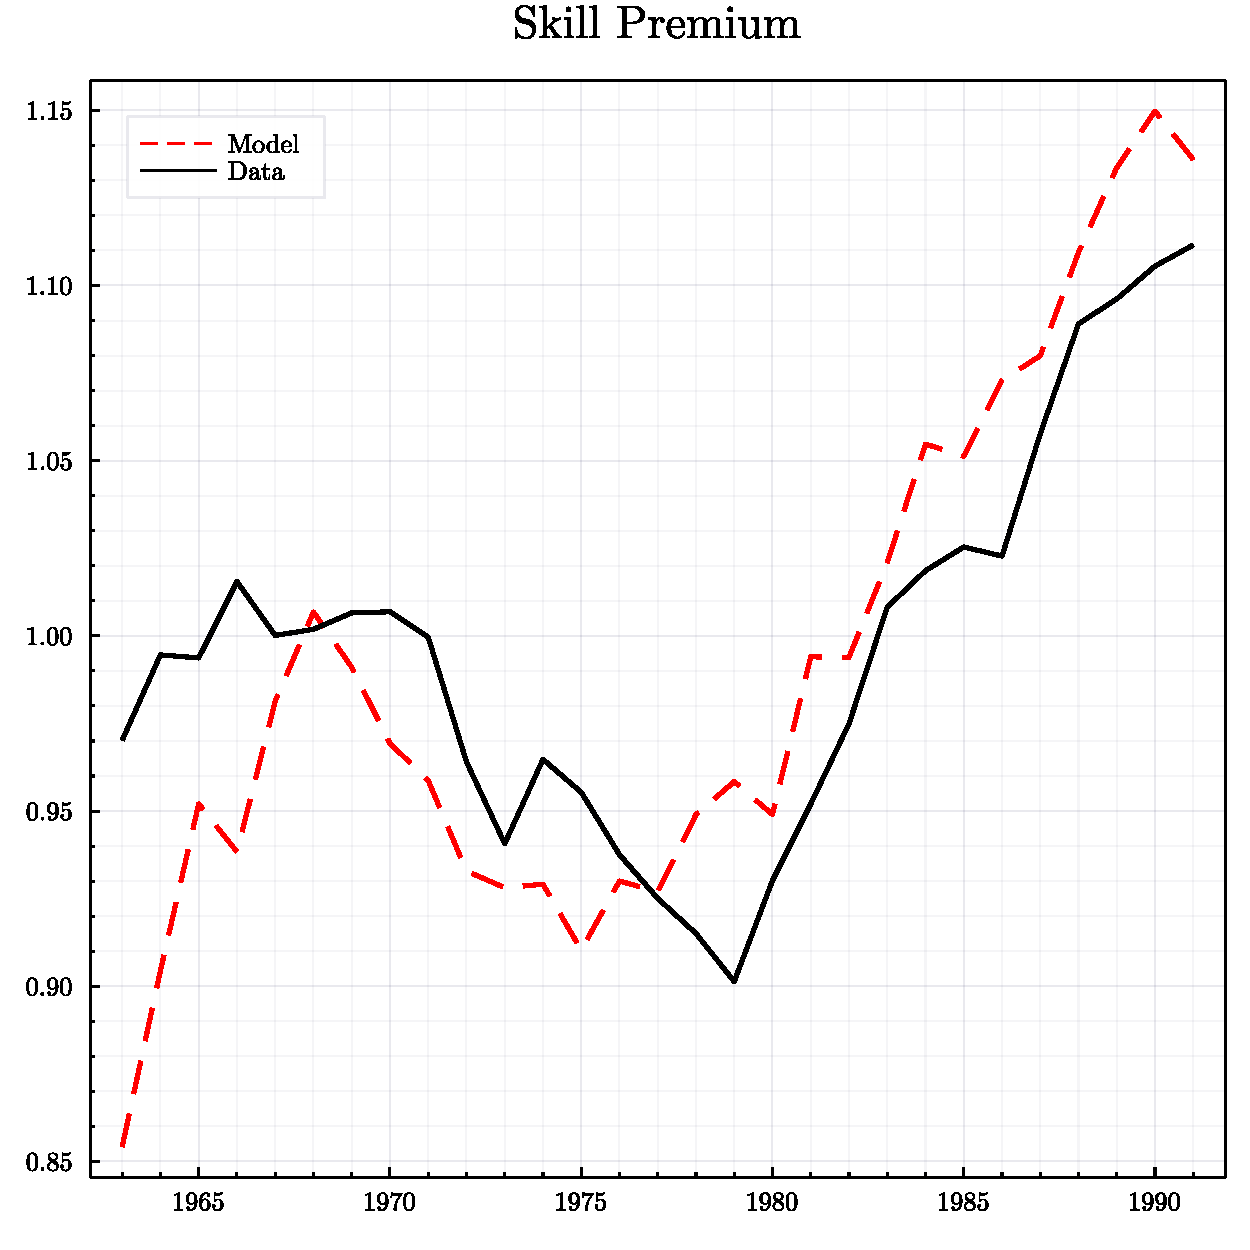
\includegraphics[width=0.3\textwidth]{../images/fig:korv_estimation_sp_doc.pdf}
 \caption{\label{fig:korv_estimation} Model Fit for 1963-1992 Period with KORV Data. Left: Labor Share (ls) of output. Center: Wage Bill Ratio (wbr), skilled compensation relative to unskilled compensation. Right: Skill Premium (sp), ratio of skilled to unskilled wages. Black lines/dots show observed data, red dashed lines show model predictions. The model closely tracks the skill premium trend and wage bill ratio but misses year-to-year volatility in the labor share.}
\end{figure}

\begin{figure}[H]
 \centering
 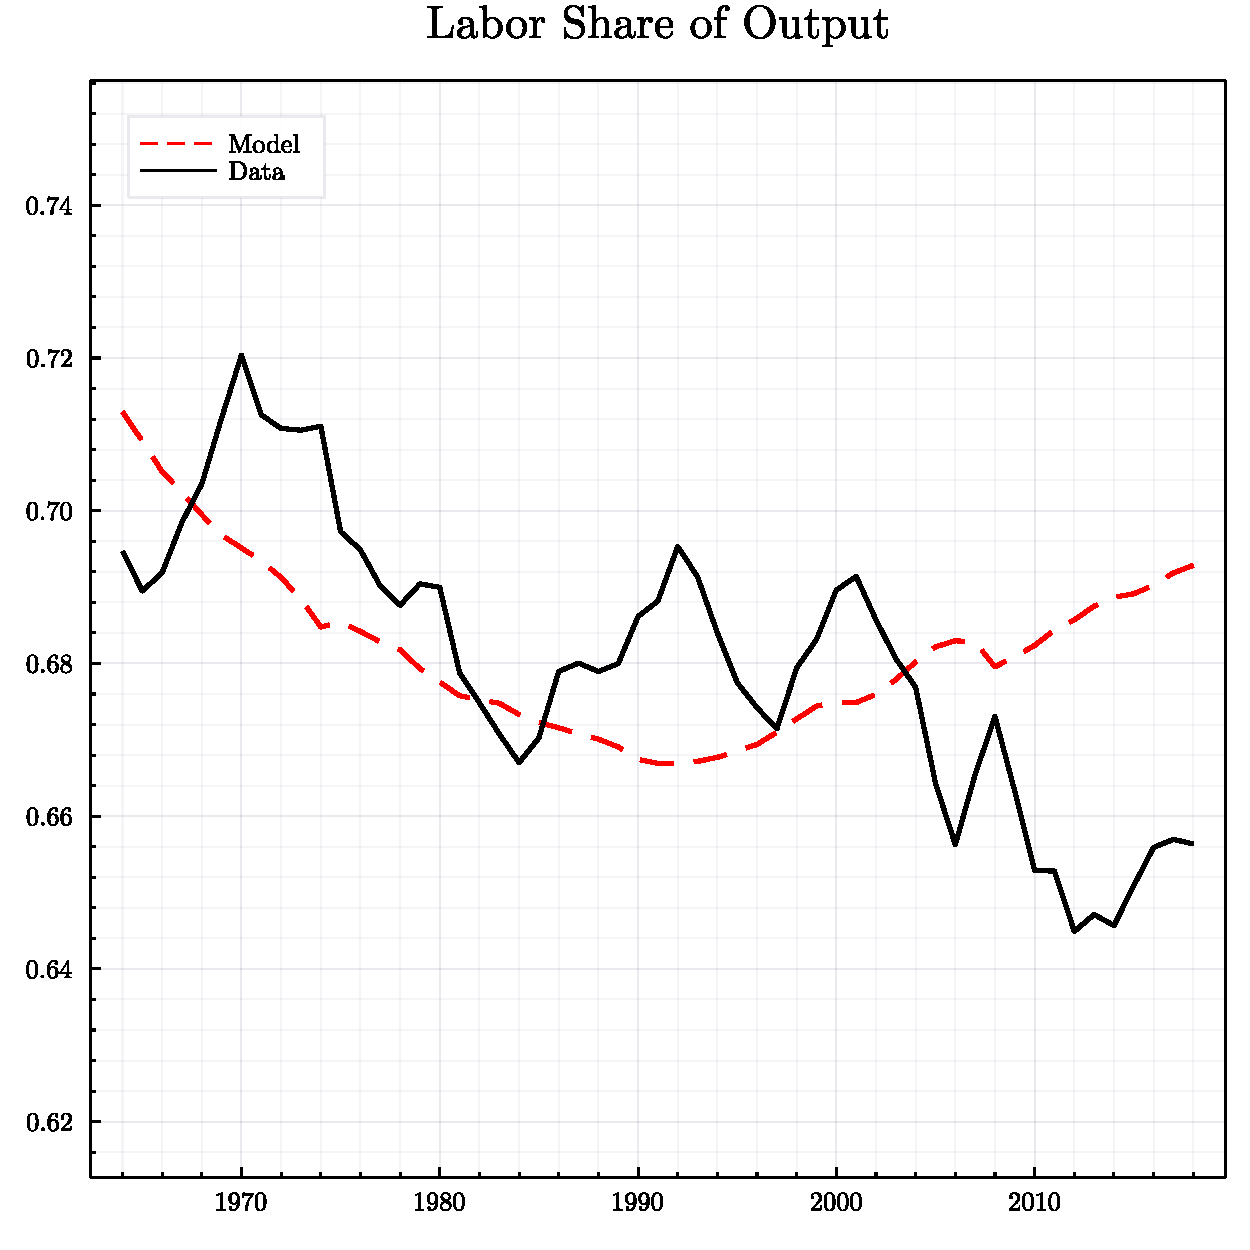
\includegraphics[width=0.3\textwidth]{../images/fig:updated_estimation_ls_doc.pdf}
 \hfill
 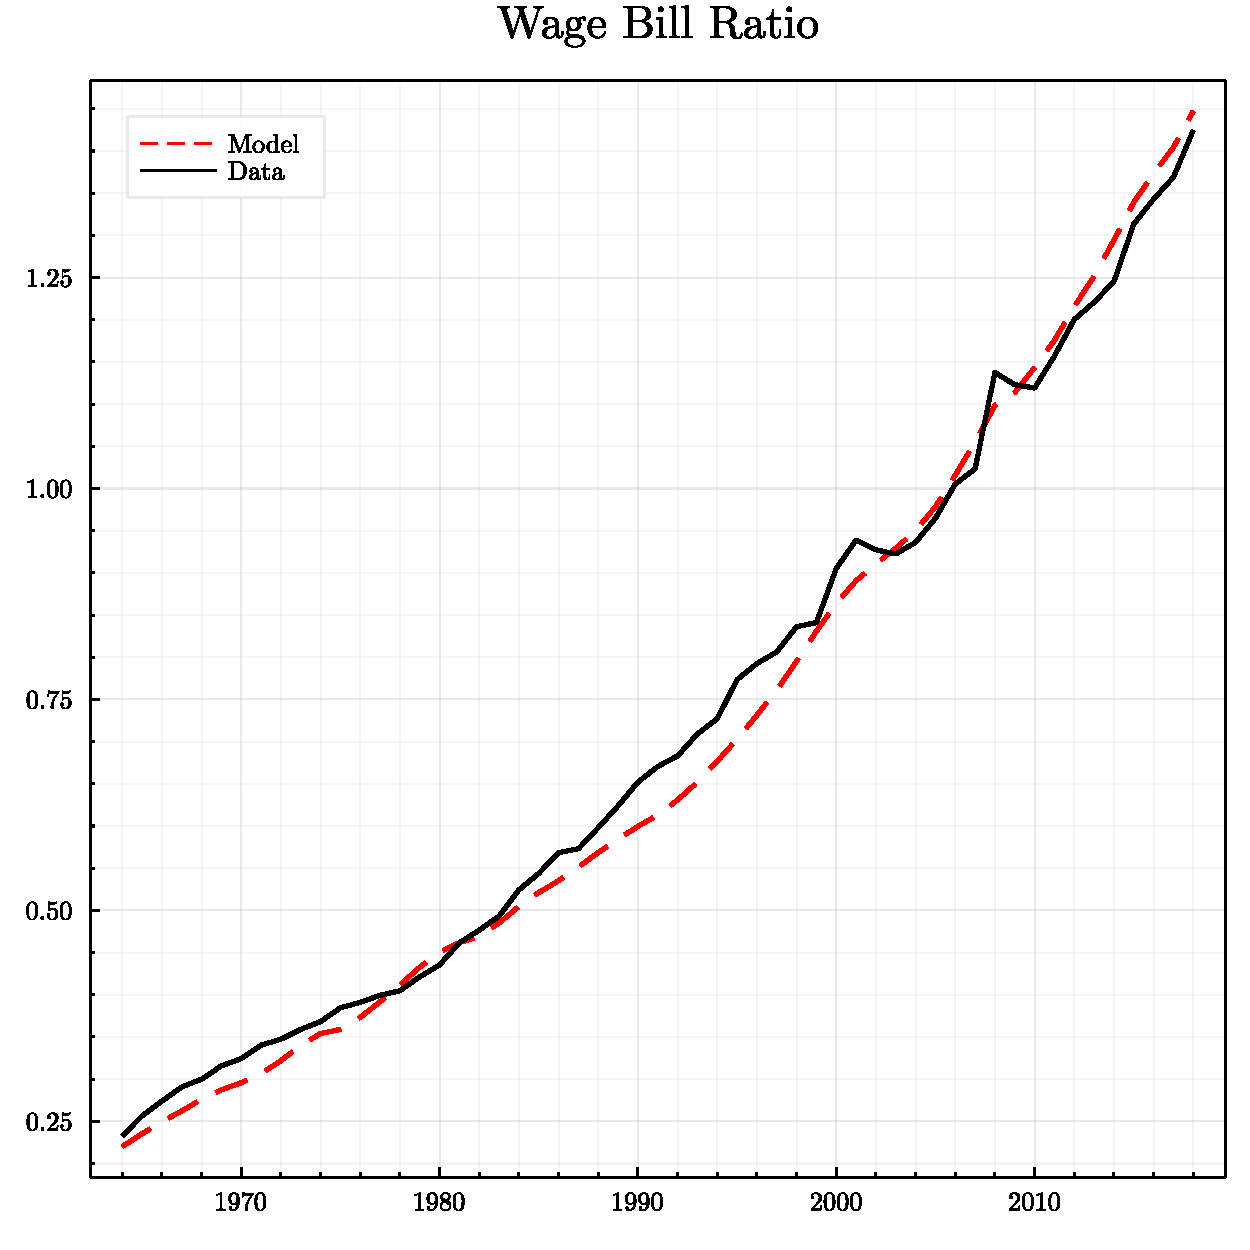
\includegraphics[width=0.3\textwidth]{../images/fig:updated_estimation_wbr_doc.pdf}
 \hfill
 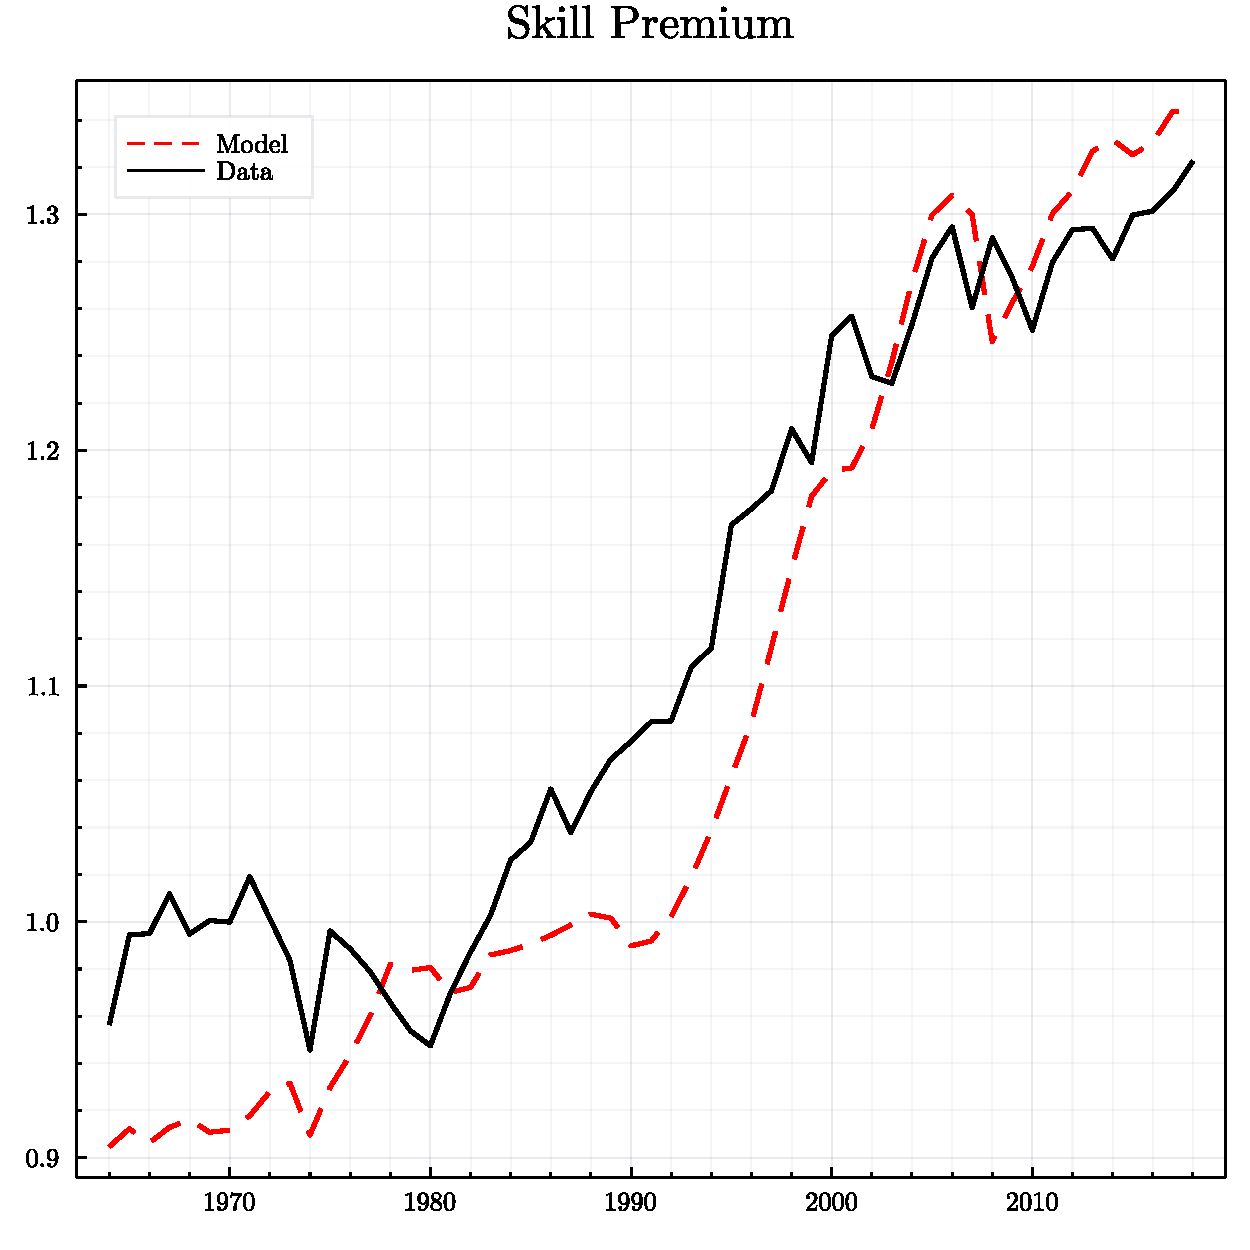
\includegraphics[width=0.3\textwidth]{../images/fig:updated_estimation_sp_doc.pdf}
 \caption{\label{fig:korv_estimation_extended} Model Fit for 1963-2018 Period with Updated Data. Left: Labor Share (ls). Center: Wage Bill Ratio (wbr). Right: Skill Premium (sp). Black lines/dots represent data, red dashed lines represent model. The extended sample shows the model struggles to capture the sharp post-2000 labor share decline, though skill premium fit remains good through 2018.}
\end{figure}
\begin{figure}[H]
 \centering
 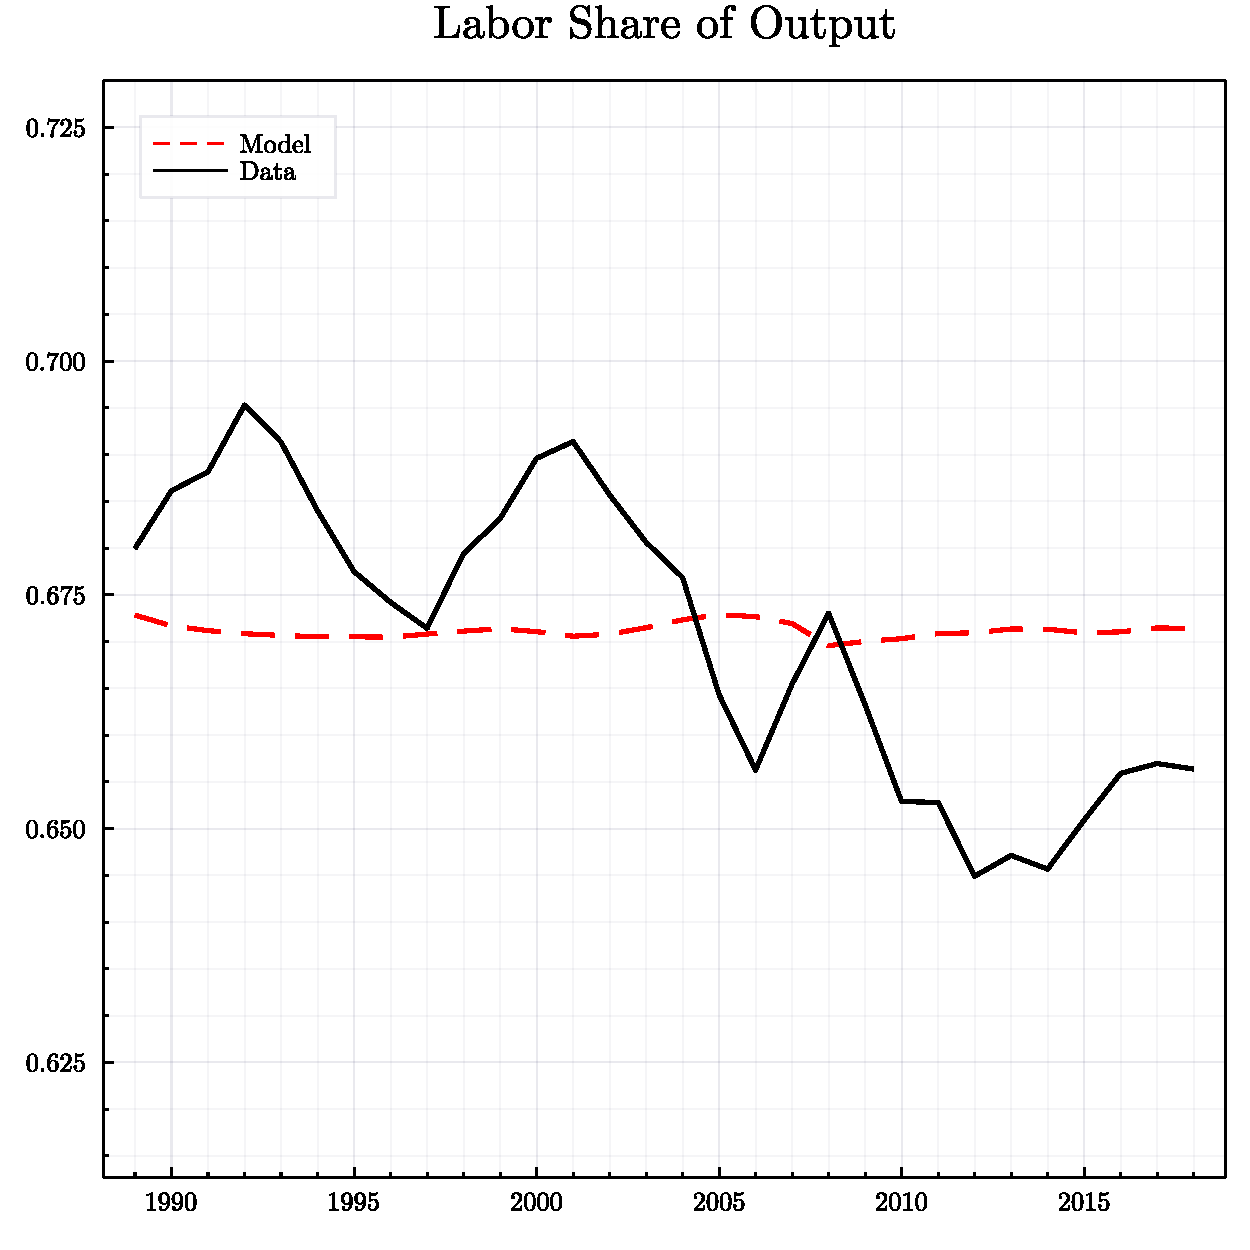
\includegraphics[width=0.3\textwidth]{../images/fig:updated_ind_estimation_ls_doc.pdf}
 \hfill
 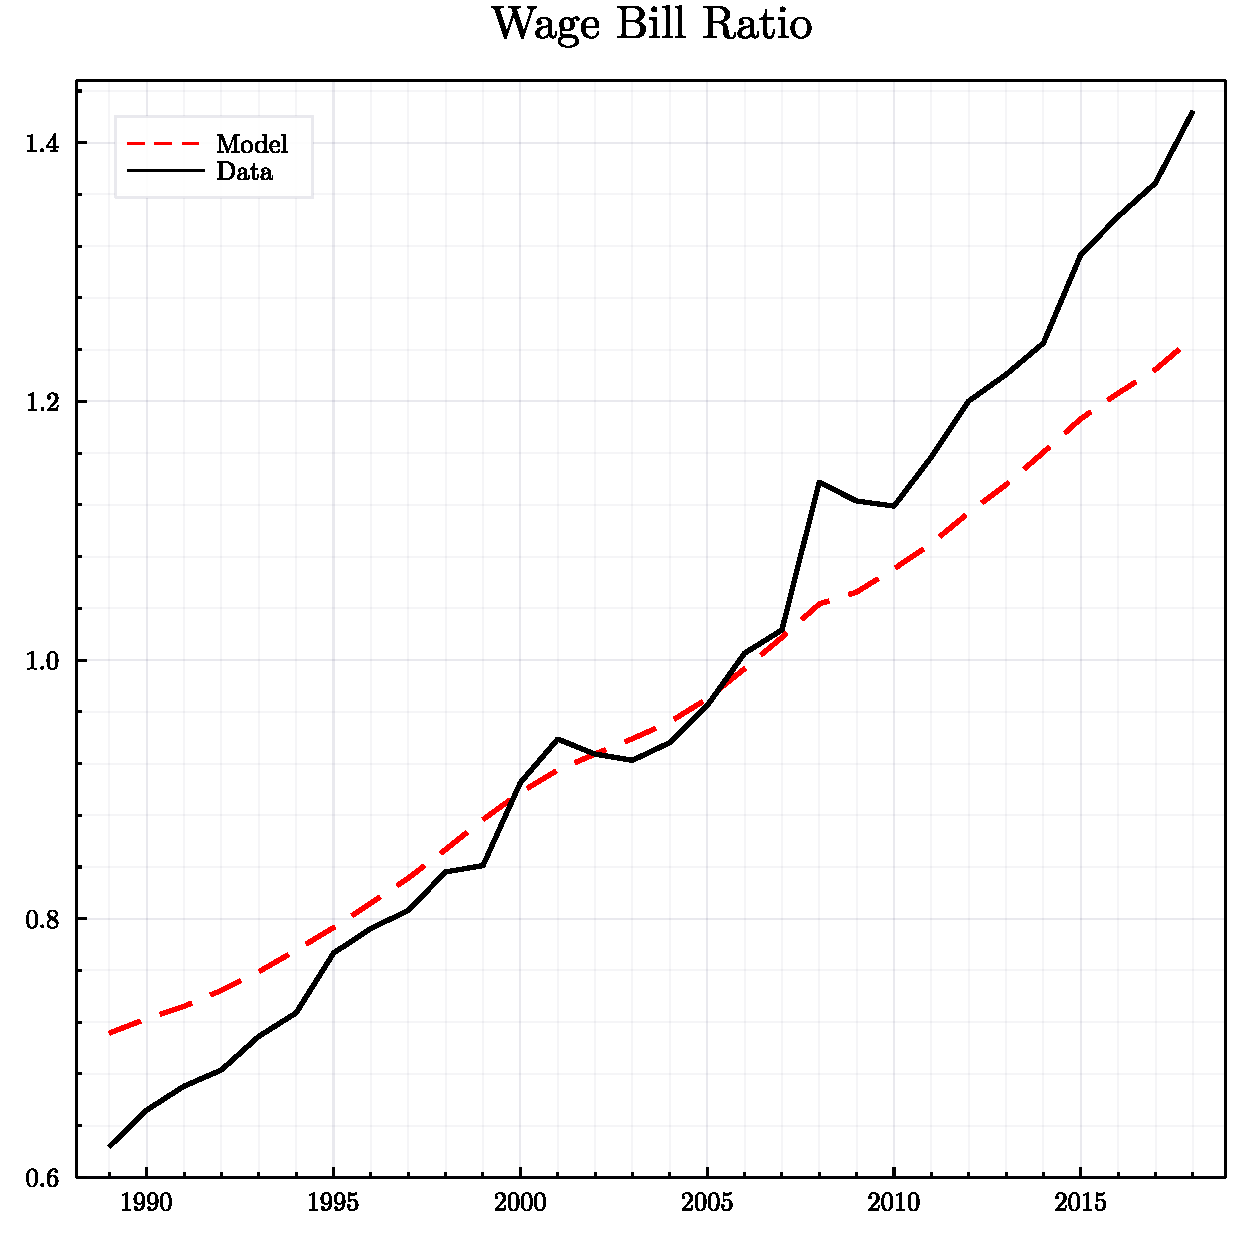
\includegraphics[width=0.3\textwidth]{../images/fig:updated_ind_estimation_wbr_doc.pdf}
 \hfill
 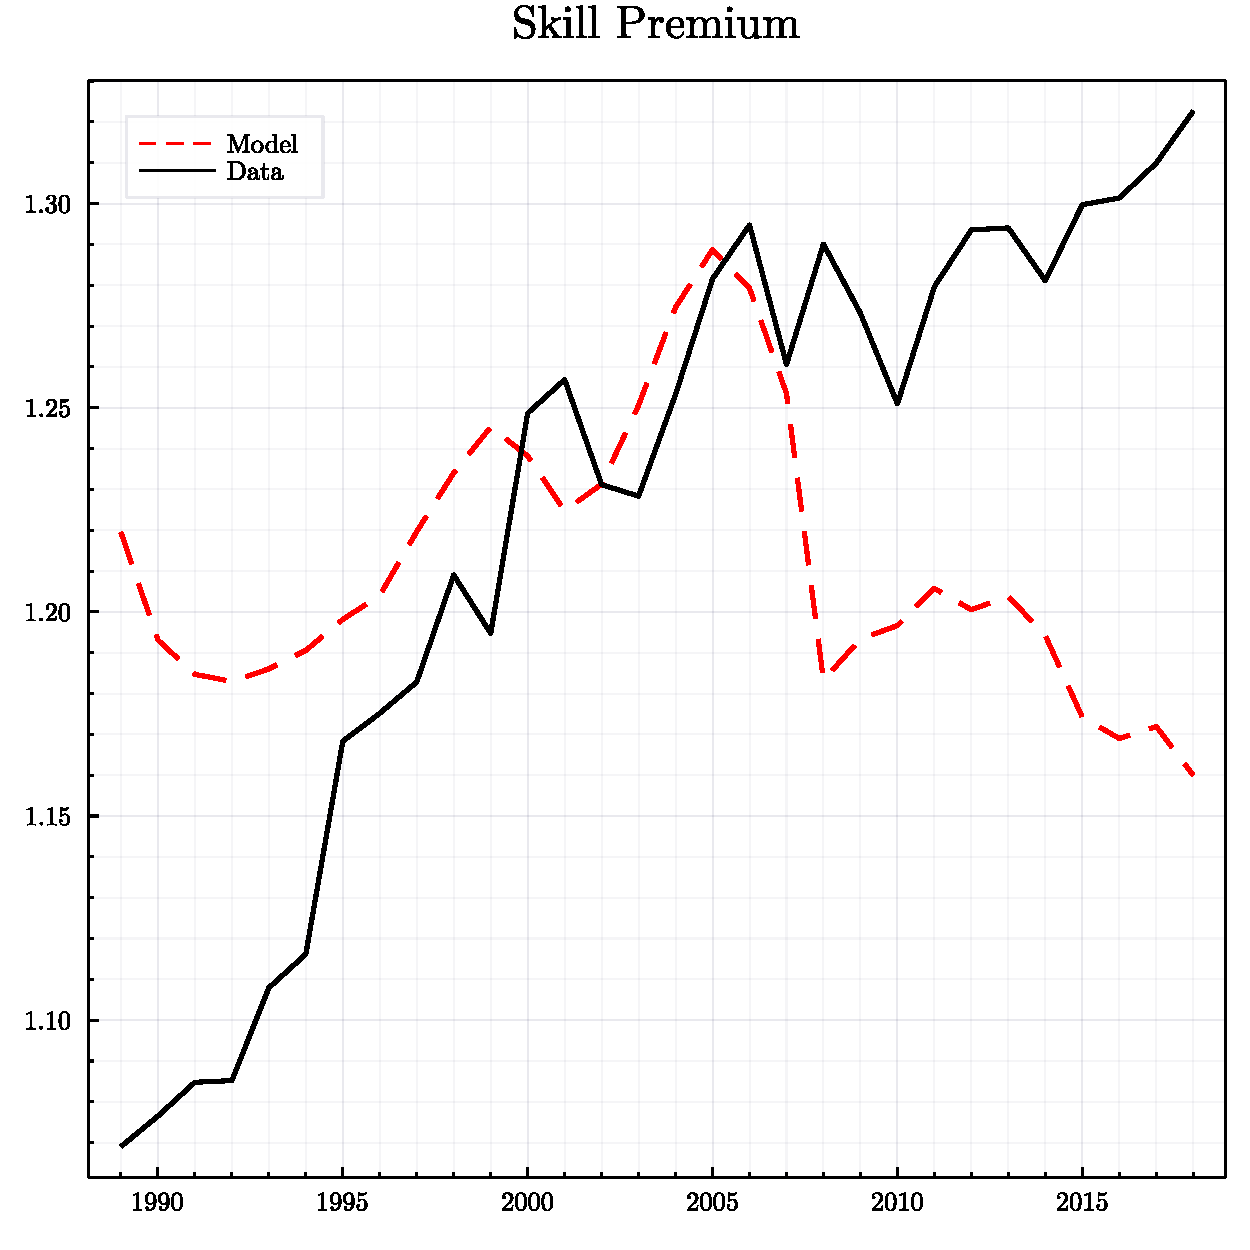
\includegraphics[width=0.3\textwidth]{../images/fig:updated_ind_estimation_sp_doc.pdf}
 \caption{\label{fig:korv_estimation_extended_industry} Model Fit for 1988-2018 Period with Updated Data. Left: Labor Share (ls). Center: Wage Bill Ratio (wbr). Right: Skill Premium (sp). Black lines/dots show data, red dashed lines show model predictions. The shorter sample reduces pre-2000 periods, making the labor share decline more prominent in the estimation window.}
\end{figure}

To quantify model fit, I compute root mean squared errors (RMSE) for a subset of industries where estimation converged successfully. For the nine industries with complete results, RMSE for the skill premium ranges from 0.20 to 2.04, with a median of 0.43. The wage bill ratio shows tighter fit, with RMSE between 0.03 and 0.68 (median 0.07). Labor share RMSE ranges from 0.03 to 0.15 (median 0.05), while relative capital prices show RMSE between 0.48 and 2.71 (median 1.24). These statistics confirm the visual impression from the figures: the model captures wage ratios and labor shares reasonably well, but struggles with high-frequency movements in prices and the skill premium in certain industries. The wide variation in fit quality across industries suggests substantial heterogeneity in technology parameters and adjustment dynamics, motivating the industry-level estimation approach discussed next.

\subsection{Estimation by Industry}

I estimate the model separately for 53 industries spanning agriculture, mining, manufacturing, trade, transportation, finance, professional services, and health care for the period 1988-2018. This industry-level analysis reveals substantial heterogeneity in production technology parameters, with $\sigma$ ranging from -3.75 to 1.00 and $\rho$ ranging from -2.23 to 1.00 across industries. The capital-skill complementarity condition ($\sigma > \rho$) holds in 44 of 53 industries (83\%), confirming that CSC is a widespread but not universal feature of U.S. production. The nine industries violating CSC include forestry, food and beverage products, and funds/trusts---sectors where skilled labor may compete directly with equipment capital for similar tasks or where intangible capital dominates over physical equipment. Table~\ref{tab:params_ind_estimates} presents the full results, showing that industries like utilities and educational services exhibit low substitution elasticities (both $\sigma$ and $\rho$ near zero), while sectors like printing, legal services, and rail transportation show near-perfect substitutability ($\sigma, \rho \approx 1$). This heterogeneity suggests that aggregating to economy-wide elasticities, as in the previous subsection, may mask important sectoral variation in how capital and labor interact, though the aggregate CSC result appears robust to this heterogeneity.

Before showing the results of the estimation at the industry level, It is important to discuss some caveats. The first issue I encountered is that the convergence of the model is highly sensitive to the initial conditions. Of the industries with available capital data, approximately 4 failed to converge to valid parameter estimates (producing NaN objective values), highlighting the numerical challenges of the SPMLE procedure in data-sparse settings. The sensitivity stems from three sources: first, the simulated likelihood surface is inherently noisy due to random shock draws, creating local optima that depend on starting values; second, the Nelder-Mead simplex algorithm used here is derivative-free and can stall in flat regions or oscillate near boundaries; third, some industry time series are short (30 observations) or exhibit structural breaks that make identification fragile---the model struggles when key moments show little variation or when trends reverse mid-sample. To assess robustness, I compare estimates across different grid points that converge to similar objective values: industries where multiple initial conditions yield nearly identical parameters (differing by less than 0.05 in $\sigma$ and $\rho$) show local identification, while those with widely varying estimates across grid points suggest weak or non-unique identification.

To deal with this problem I implement a strategy of sweeping the parameter space for suitable initial conditions with high tolerance to get an initial approximation and then select the best initial condition based on the value of the objective function (equation~\eqref{eq:objective_funct_estimation}). The grid search explores combinations of $\sigma \in \{0.5, -0.45\}$, $\rho \in \{-0.5, 0.45\}$, $\eta_\omega \in \{0.01, 0.04, 0.3\}$, $\phi_L = 4.0$, $\phi_H = 6.0$, $\lambda = 0.4$, and $\mu = 0.4$, subject to the CSC constraint $\sigma > \rho$ (non-CSC combinations are excluded). This yields multiple starting points per industry, with each run using tolerance $10^{-2}$ and maximum 300 iterations. After convergence from all grid points, I select the parameter vector achieving the lowest objective function value as the industry's estimate. While this brute-force approach is computationally intensive (requiring several estimation runs per industry), it mitigates the risk of reporting a poor local optimum and provides informal evidence on identification by revealing whether different starting values converge to a common parameter region. Table~\ref{tab:estimation_ind} presents a summary of the results of the estimation process at the industry level.

 \begin{table}[h]
 \begin{center}
 \begin{tabular}{rrrrr}
 \hline\hline
 & \textbf{Updated Data} & \textbf{Industry Level} & \textbf{Industry Level} \\
 & \texttt{$1988$ - $2018$} & \texttt{(mean)} & \texttt{(std)} \\
 \hline
 $\alpha$ & 0.08 & 0.241 & 0.206 \\
 $\sigma$ & 0.313 & 0.483 & 0.710\\
 $\rho$ & -0.154 & -0.289 & 0.816\\
 $\eta_\omega$& 0.043 & 0.131 & 0.195\\
 \hline\hline
 \end{tabular}
\end{center}
\caption{\label{tab:estimation_ind} Summary Industry Level Estimates.}
\end{table}

The substantial divergence between industry-level parameter estimates and the aggregate benchmark reveals both true technological heterogeneity and potential aggregation bias. Comparing the mean industry estimates to the aggregate (1988-2018 column), capital intensity $\alpha$ averages 0.241 across industries versus 0.08 at the aggregate level, while $\sigma$ averages 0.483 versus 0.313 aggregate. This pattern suggests classic aggregation bias: when production technologies differ across sectors, aggregate elasticities represent a complex weighted average that depends on industry sizes, factor shares, and covariances between quantities and prices---not a simple mean of industry parameters. The aggregate estimate mechanically downweights industries with extreme parameters or small employment shares, while industries near the technological "center" receive disproportionate influence. The enormous standard deviations---$\sigma$ varies with std dev 0.710, $\rho$ with std dev 0.816---indicate genuine technological diversity rather than pure estimation noise: industries span the full range from capital-intensive manufacturing (high $\alpha$) to labor-intensive services (low $\alpha$), and from routine-task sectors where automation substitutes easily for workers (high $\sigma$) to professional services where human judgment remains essential (low $\sigma$). Preliminary analysis suggests potential industry clusters: resource extraction and heavy manufacturing (mining, petroleum, primary metals) exhibit high capital intensity and strong substitutability; professional and business services (legal, accounting, consulting) show moderate capital intensity with pronounced skill complementarity; while education, health care, and hospitality display low capital intensity and weak substitution patterns, consistent with the inherently labor-intensive, human-interaction-focused nature of these services. These clusters align with intuition about production technologies but require formal statistical testing (e.g., cluster analysis or mixture models) to establish rigorously.

\begin{figure}[H]
 \centering
 \includegraphics[width=\textwidth]{../images/parameter_distributions_comprehensive.pdf}
 \caption{\label{fig:parameter_distributions} Parameter Distributions Across Industries. Histograms show the distribution of estimated parameters across 54 industries with kernel density overlays. Panel A shows the equipment-unskilled substitution elasticity parameter $\sigma$, Panel B the equipment-skilled substitution parameter $\rho$, Panel C the CSC strength $\sigma - \rho$, Panel D the structures share $\alpha$, and Panels E-F show the implied elasticities of substitution $\sigma_s = 1/(1-\rho)$ and $\sigma_u = 1/(1-\sigma)$. Dashed vertical lines indicate means, dotted lines indicate medians. Note that extreme elasticity values (7 industries with $|\sigma_s|$ or $|\sigma_u| > 50$) are excluded from Panels E-F for visual clarity. The distributions reveal substantial heterogeneity: $\sigma$ ranges from -3.7 to 1.0, $\rho$ from -2.2 to 1.0, with CSC ($\sigma > \rho$) holding in 44 of 54 industries (81\%).}
\end{figure}

To understand which industries exhibit the most extreme production technologies, Table~\ref{tab:extreme_csc_industries} presents the top and bottom 10 industries ranked by CSC strength ($\sigma - \rho$). Industries with the strongest complementarity---computer systems design (5415), legal services (5411), management services (55), and miscellaneous professional services (5412OP)---are all knowledge-intensive sectors where information technology augments rather than replaces skilled workers. These industries exhibit high average skill premiums (2.0-2.7) and skilled-to-unskilled labor ratios (1.5-6.5), consistent with production processes where computers enhance the productivity of lawyers, consultants, and IT professionals but cannot fully substitute for their expertise. Conversely, industries with the weakest or negative CSC---food manufacturing (311FT), funds and trusts (525), petroleum refining (324), and apparel (315AL)---span both traditional manufacturing with routine production tasks amenable to automation and financial sectors where algorithmic trading may substitute for skilled analysts. The pattern suggests that CSC is strongest in industries requiring human judgment, creativity, and complex problem-solving, while weakest in sectors with standardizable processes or where both skilled and unskilled workers face similar automation risks.

\begin{table}[H]
\caption{Industries with Extreme Capital-Skill Complementarity}
\label{tab:extreme_csc}
\begin{center}
\small
\begin{tabular}{lccc|lccc}
\toprule
\multicolumn{4}{c}{\textbf{Strongest CSC (Top 10)}} & \multicolumn{4}{c}{\textbf{Weakest CSC (Bottom 10)}} \\
\cmidrule(lr){1-4} \cmidrule(lr){5-8}
Industry & $\sigma$ & $\rho$ & $\sigma-\rho$ & Industry & $\sigma$ & $\rho$ & $\sigma-\rho$ \\
\midrule
Hospitals and nursing and residential care facilities & 0.71 & -2.23 & 2.94 & Rail transportation & 0.99 & 0.99 & 0.00 \\
Textile mills and textile product mills & 0.99 & -1.46 & 2.45 & Printing and related support activities & 1.00 & 1.00 & 0.00 \\
Electrical equipment, appliances, and components & 0.99 & -1.21 & 2.20 & Forestry, fishing, and related activities & -0.57 & -0.55 & -0.02 \\
Management of companies and enterprises & 0.56 & -1.25 & 1.81 & Primary metals & 0.97 & 0.99 & -0.02 \\
Social assistance & 0.32 & -1.39 & 1.71 & Oil and gas extraction & 0.98 & 1.00 & -0.02 \\
Truck transportation & 1.00 & -0.61 & 1.61 & Wood products & 0.84 & 0.93 & -0.09 \\
Miscellaneous professional, scientific, and technical services & 0.66 & -0.90 & 1.56 & Water transportation & 0.46 & 0.64 & -0.18 \\
Computer systems design and related services & 0.90 & -0.64 & 1.53 & Apparel and leather and allied products & 0.72 & 1.00 & -0.27 \\
Air transportation & 0.45 & -0.99 & 1.45 & Ambulatory health care services & 0.68 & 0.96 & -0.29 \\
Farms & 0.49 & -0.92 & 1.41 & Funds, trusts, and other financial vehicles & -3.75 & 0.44 & -4.18 \\
\bottomrule
\end{tabular}
\end{center}
\begin{minipage}{\textwidth}
\small
\textit{Note:} Left panel shows industries with highest $\sigma - \rho$ (strongest complementarity). Right panel shows lowest $\sigma - \rho$ (weakest or negative complementarity).
\end{minipage}
\end{table}


Figure~\ref{fig:estimation_5411} show the fit obtained for a specific industry (Legal Services). Appendix~\ref{sec:industry-trends} shows the fit for all industries. The model can replicate the pattern and shape of the skill premium but fails to generate the volatility present in the Labor Share of Output. In general, the model can match the growth patterns of the skill premium but sometimes fails to correctly match the levels. The explanation is that the skill premium is not a target of the estimation process and I choose initial conditions to minimize the objective function instead of the ones that give a better fit for the skill premium series. Focusing on growth rates rather than levels is appropriate for my research question because the decomposition in equation~\eqref{eq:skill_premium_growth_rates} identifies the contributions of supply, demand, and CSC channels from the co-movement of skill premiums with relative factor quantities---not from absolute levels. The initial skill premium level is largely determined by historical conditions and institutional factors outside the model, while growth rates capture the technological and supply responses that are the focus of the analysis. Adding the skill premium level as an additional moment would either over-identify the system (requiring elimination of another moment) or demand additional parameters, risking overfitting. The current approach prioritizes matching labor market quantities (labor share, wage bill ratio, labor input ratio) that directly discipline the production function elasticities, accepting some sacrifice in skill premium levels to ensure robust identification of the structural parameters governing factor substitution.

Model fit quality varies systematically across industries, providing insights into which sectors are well-described by the nested CES framework and which may require extensions. Table~\ref{tab:fit_quality_summary} summarizes fit statistics by tercile: industries in the "Good" fit category achieve average $R^2$ of 0.74 for the wage bill ratio and -0.05 for the skill premium, with average RMSE of 0.21 (skill premium) and 0.06 (labor share). "Poor" fit industries exhibit dramatically worse performance: average $R^2$ of -41.7 for wage bill ratio and -528.4 for skill premium, indicating the model systematically fails to capture variation in these series. The poor $R^2$ values for skill premium even in well-fit industries reflect the aforementioned focus on growth rates over levels, while the labor input ratio achieves perfect $R^2 = 1.0$ across all categories because it is mechanically determined by the wage bill ratio and skill premium. Industries with the best fit (Table~\ref{tab:best_worst_fit})---wholesale trade (42), utilities (22), and electrical equipment (335)---tend to have longer time series, stable production processes, and clear technology adoption patterns. Industries with the worst fit---petroleum refining (324), funds/trusts (525), and transit (485)---often have short sample periods, experienced major structural shifts (financial deregulation, shale oil boom), or exhibit volatile year-to-year fluctuations driven by commodity prices or regulatory changes. This pattern suggests the basic nested CES model performs best for industries with gradual technological change and stable factor demands, while industries subject to major disruptions or market power considerations may require extensions incorporating adjustment costs, imperfect competition, or globalization channels.

\begin{table}[H]
\caption{Summary of Model Fit Quality by Category}
\label{tab:fit_quality_summary}
\begin{center}
\begin{tabular}{lccccc}
\toprule
Fit Category & N & \multicolumn{4}{c}{Mean RMSE} \\
\cmidrule(lr){3-6}
& & Skill Prem. & Labor Share & Wage Bill Ratio & Labor Input Ratio \\
\midrule
Good & 18 & 0.207 & 0.058 & 0.098 & 0.000 \\
Medium & 18 & 0.315 & 0.060 & 0.153 & 0.000 \\
Poor & 18 & 2.009 & 0.123 & 4.107 & 0.000 \\
\midrule
\multicolumn{6}{l}{\textbf{Mean $R^2$ by Category}} \\
\midrule
Good & 18 & -0.481 & -0.045 & 0.741 & 1.000 \\
Medium & 18 & -3.962 & -1.313 & 0.259 & 1.000 \\
Poor & 18 & -528.422 & -17.393 & -41.718 & 1.000 \\
\bottomrule
\end{tabular}
\end{center}
\begin{minipage}{\textwidth}
\small
\textit{Note:} Industries classified into terciles based on overall fit quality (average $R^2$ across four series). 
Good fit = top tercile, Medium = middle tercile, Poor = bottom tercile. RMSE and $R^2$ averaged across industries within each category.
\end{minipage}
\end{table}


\begin{table}[H]
\caption{Industries with Best and Worst Model Fit}
\label{tab:best_worst_fit}
\begin{center}
\small
\begin{tabular}{lcc|lcc}
\toprule
\multicolumn{3}{c}{\textbf{Best Fit (Top 10)}} & \multicolumn{3}{c}{\textbf{Worst Fit (Bottom 10)}} \\
\cmidrule(lr){1-3} \cmidrule(lr){4-6}
Industry & Avg $R^2$ & Avg RMSE & Industry & Avg $R^2$ & Avg RMSE \\
\midrule
Accommodation & 0.618 & 0.058 & Rental and leasing services and lessors of intangible assets & -14.933 & 0.222 \\
Printing and related support activities & 0.574 & 0.217 & Miscellaneous professional, scientific, and technical services & -15.563 & 0.583 \\
Oil and gas extraction & 0.559 & 0.105 & Social assistance & -20.093 & 0.194 \\
Rail transportation & 0.545 & 0.067 & Computer systems design and related services & -22.300 & 0.936 \\
Motor vehicles, bodies and trailers, and parts & 0.494 & 0.077 & Hospitals and nursing and residential care facilities & -31.578 & 0.300 \\
Transit and ground passenger transportation & 0.474 & 0.069 & Other services, except government & -85.237 & 0.334 \\
Utilities & 0.412 & 0.039 & Educational services & -94.762 & 0.540 \\
Construction & 0.386 & 0.030 & Apparel and leather and allied products & -186.089 & 1.878 \\
Broadcasting and telecommunications & 0.355 & 0.068 & Truck transportation & -427.899 & 1.195 \\
Nonmetallic mineral products & 0.311 & 0.068 & Funds, trusts, and other financial vehicles & -1684.451 & 17.899 \\
\bottomrule
\end{tabular}
\end{center}
\begin{minipage}{\textwidth}
\small
\textit{Note:} Avg $R^2$ and Avg RMSE computed as averages across skill premium, labor share, wage bill ratio, and labor input ratio. 
Higher $R^2$ indicates better fit; lower RMSE indicates better fit.
\end{minipage}
\end{table}


\begin{figure}[H]
 \centering
 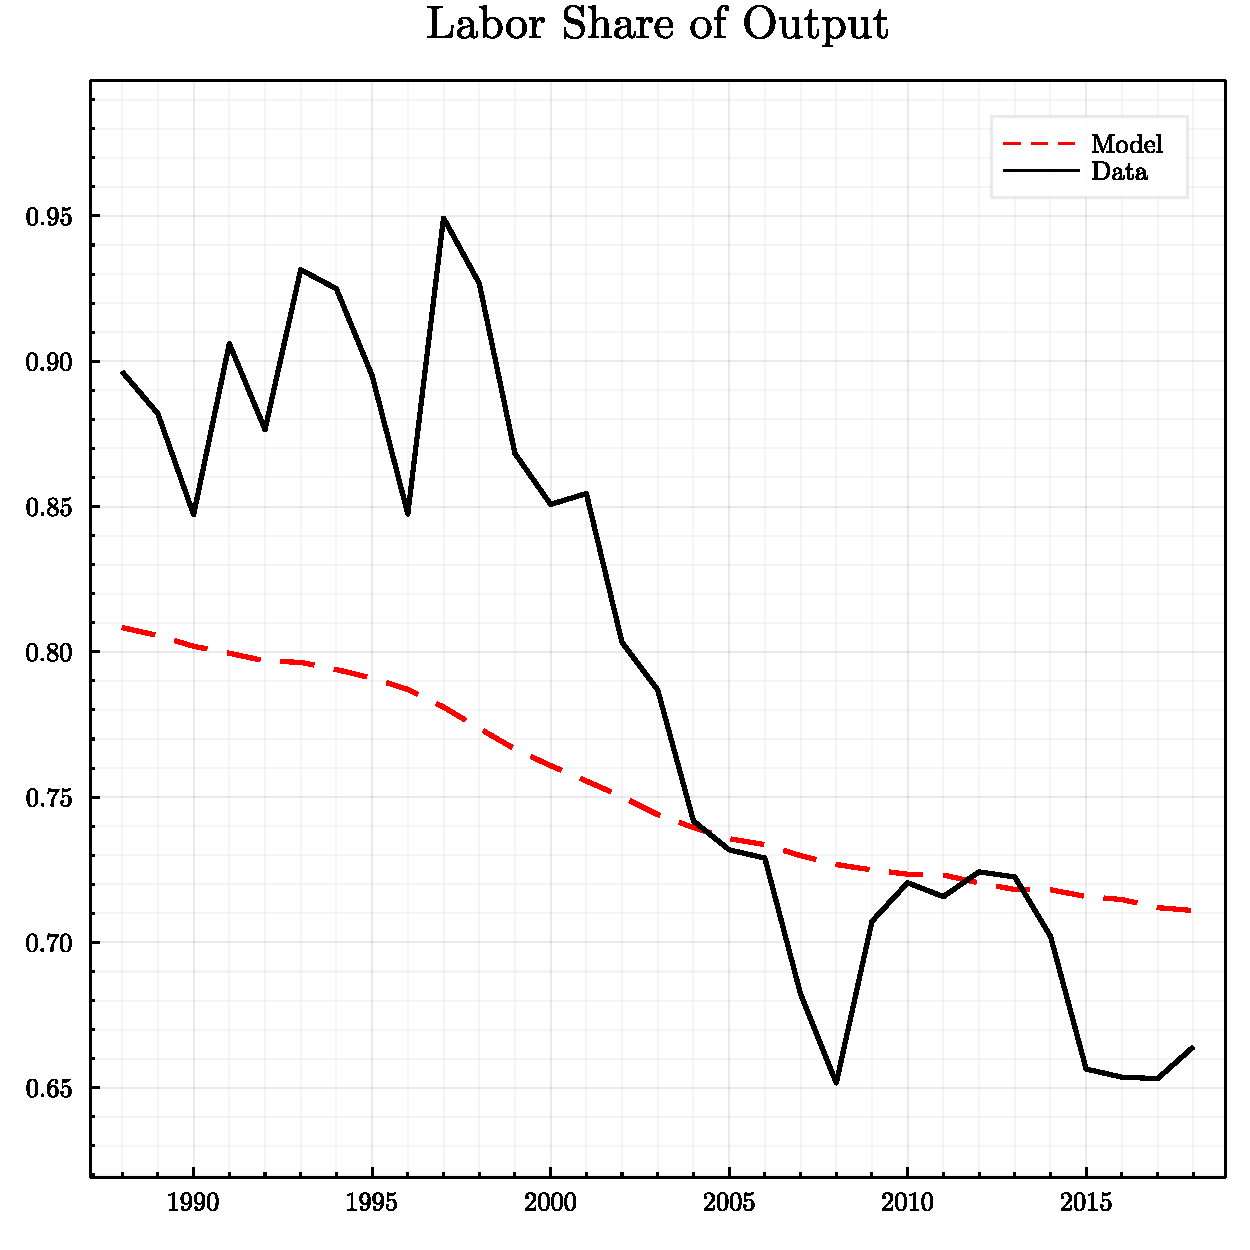
\includegraphics[width=0.3\textwidth]{../images/fig_ind_5411_estimation_ls_doc.pdf}
 \hfill
 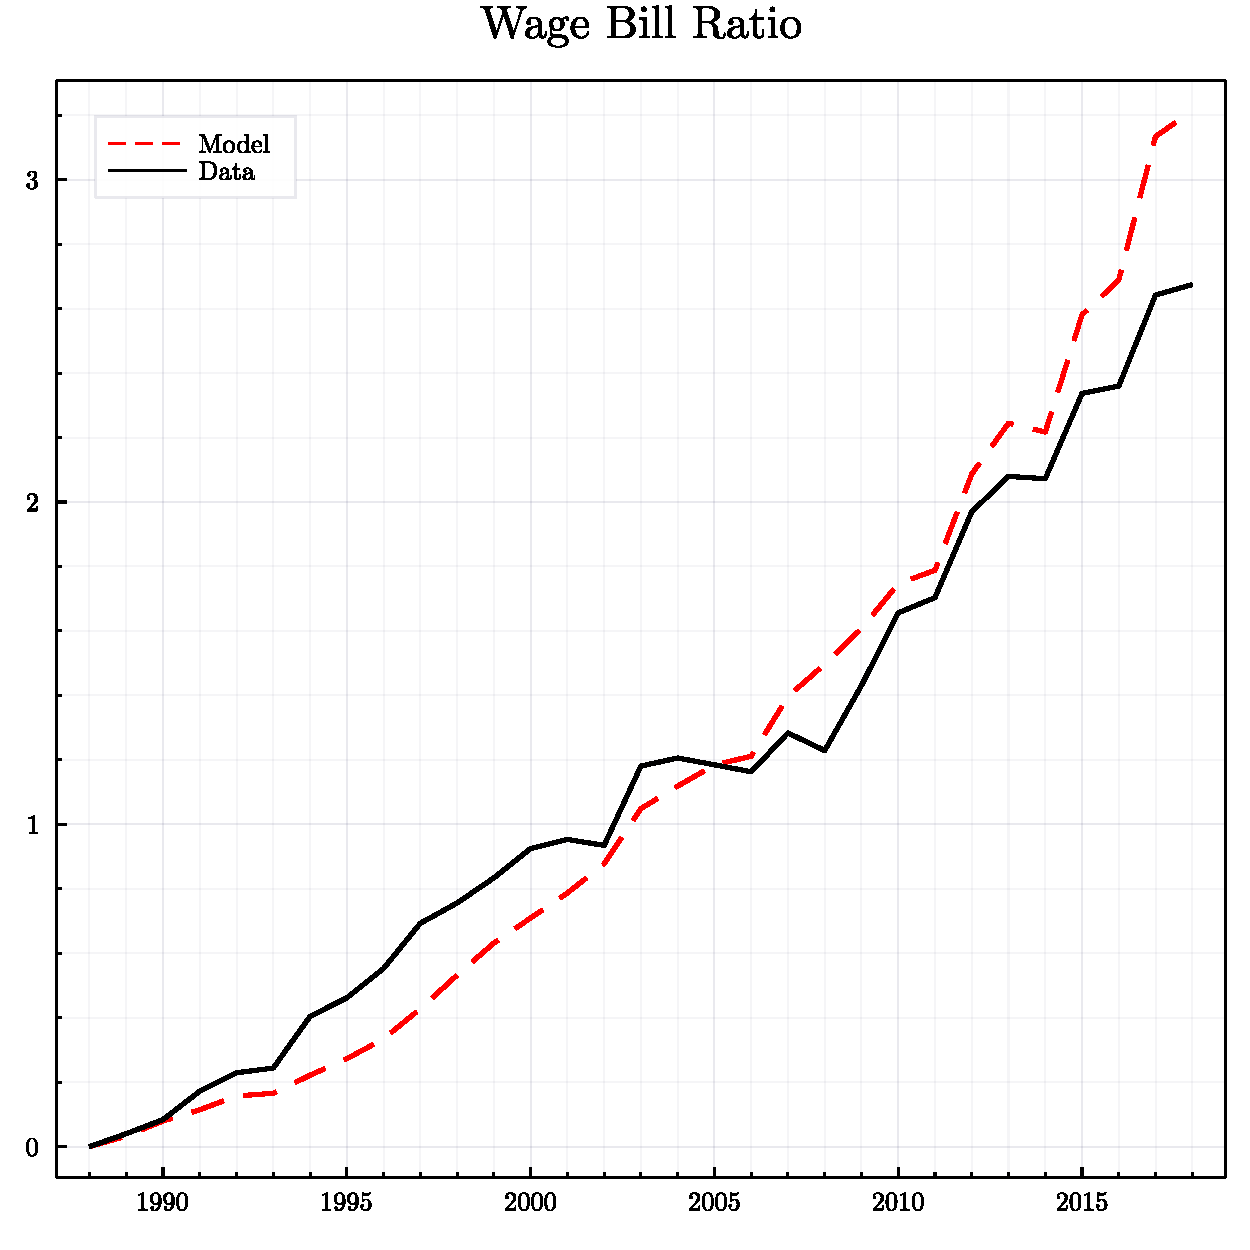
\includegraphics[width=0.3\textwidth]{../images/fig_ind_5411_estimation_wbr_doc.pdf}
 \hfill
 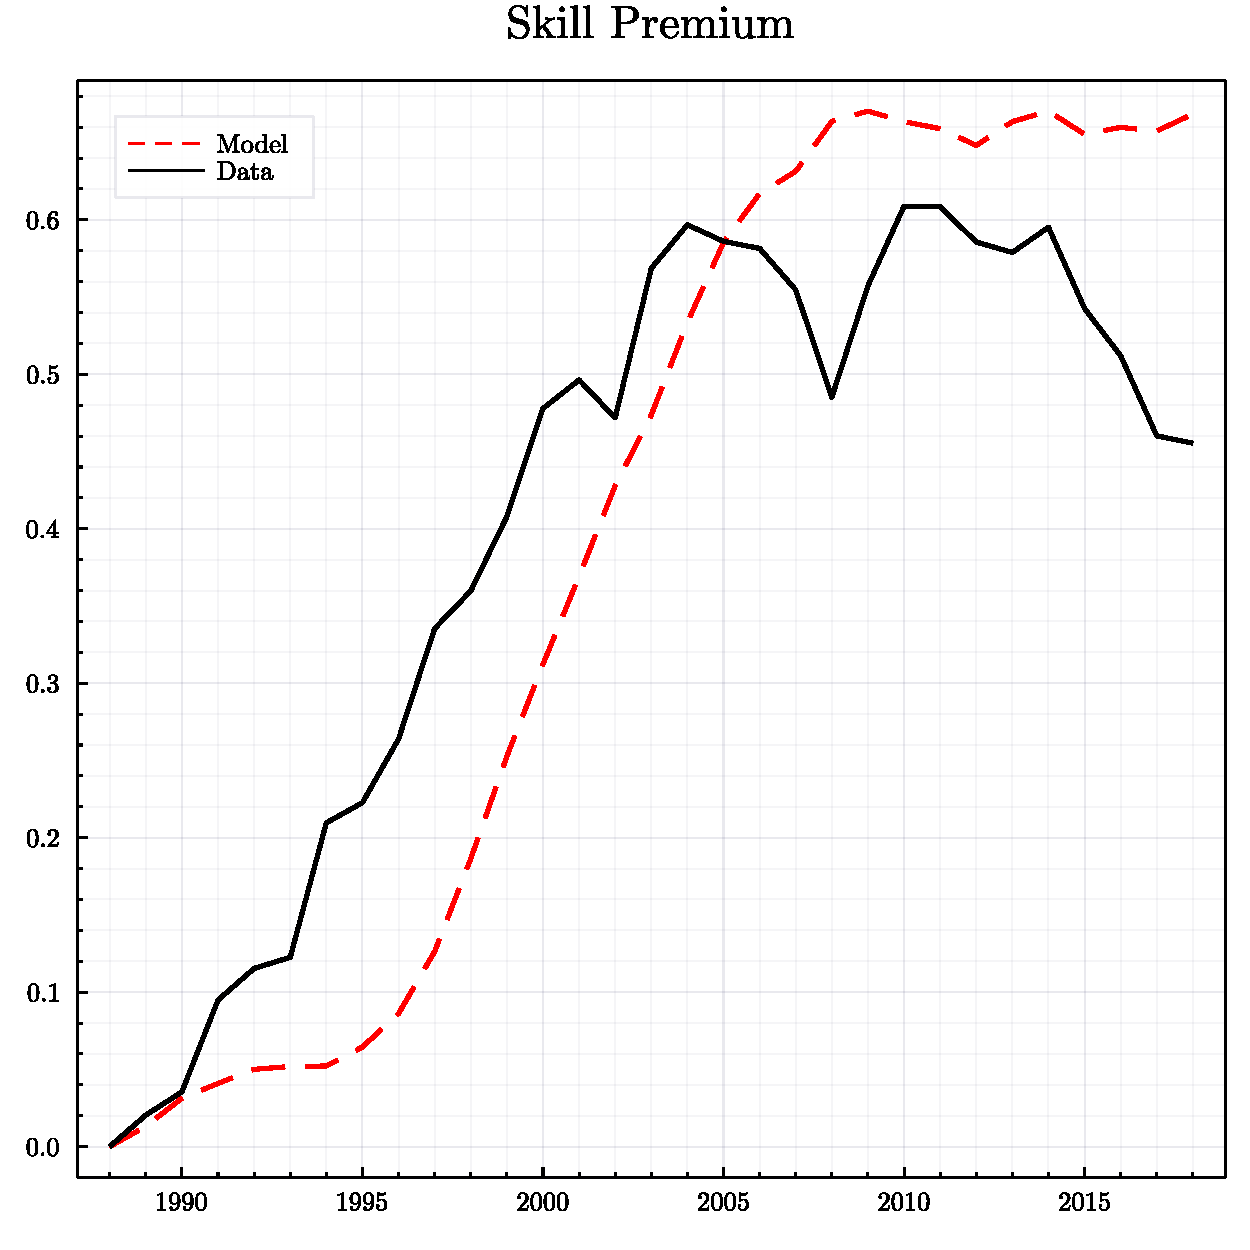
\includegraphics[width=0.3\textwidth]{../images/fig_ind_5411_estimation_sp_doc.pdf}
 \caption{\label{fig:estimation_5411} Fit for the $1988$ - $2018$ period. Legal Services Industry. Legal services illustrates an industry with extreme capital-skill complementarity ($\sigma = 1.0, \rho = 0.112$), representing the upper bound of near-perfect substitutability between equipment and unskilled labor combined with modest complementarity with skilled labor. This industry is representative of professional services sectors where highly educated workers (lawyers, paralegals) use information technology extensively but remain difficult to fully automate, while support staff tasks have been largely computerized. The model captures the broad trends in labor share and wage bill ratio reasonably well, though it misses some year-to-year volatility, typical of the fit quality across most industries.}
\end{figure}

On average the Capital-skill complementarity hypothesis $(\sigma > \rho)$ holds at the industry level.
Specifically, the hypothesis holds for $44$ of $56$ ($78.8\%$) industries. In general, the point estimates of the parameters show high variance across industries. Although not statistically significant, the strength of the capital-skill complementarity hypothesis is captured as the difference $\sigma - \rho$ increases in industries with higher skill premiums and with a higher proportion of skilled workers. Table~\ref{tab:reg_csc} summarizes the results of the regression and Figure~\ref{fig:trends_correlation_csc} shows the relationship between the difference $\sigma - \rho$, the skill premium (left) and labor input ratio (right). The lack of statistical significance likely reflects three factors: first, the small sample size (56 industries) provides limited power to detect relationships, especially given the substantial parameter heterogeneity documented above; second, measurement error in both the estimated elasticities (which themselves come from noisy industry-level estimation with convergence challenges) and the industry-level skill premium measures (calculated from CPS data with modest industry sample sizes) attenuates the estimated correlations toward zero. Despite the statistical insignificance, the economic magnitudes are meaningful: the point estimates suggest that a one-unit increase in the labor input ratio (skilled/unskilled workers) is associated with a 7.8 percentage point increase in $\sigma - \rho$, representing a substantial shift in production technology if causal. The relationship may also exhibit non-linearities: industries might need to exceed a threshold level of skill intensity before capital-skill complementarity becomes economically important, or the relationship could be driven by a subset of high-tech industries where both skill intensity and CSC are extreme, suggesting future work should explore potential threshold effects or industry clusters.

To quantify the relative importance of supply versus demand forces in driving skill premium changes, I apply the decomposition from equation~\eqref{eq:skill_premium_growth_rates} to each industry using the estimated structural parameters. This decomposition separates the observed skill premium growth into three components: the supply effect (changes in relative skill supply $H_s/H_u$, which tends to reduce premiums), the capital-skill complementarity effect (changes in the equipment-to-structures ratio $K_{eq}/K_{str}$ interacting with the difference $\sigma - \rho$, which tends to raise premiums when CSC holds), and the efficiency effect (changes in relative productivity $A_s/A_u$, capturing residual shifts). Successfully decomposing 28 of 32 industries (87.5\%), the results provide strong evidence that the CSC channel dominates: in 22 of 28 industries (78.6\%), the capital-skill complementarity effect exceeds the supply effect in absolute magnitude. The median CSC contribution is 1261\% while the median supply contribution is -685\%, with percentages exceeding $\pm$100\% because multiple forces work in opposing directions and must sum to 100\% within each industry. In absolute terms, typical magnitudes are more interpretable: industries like wholesale trade, utilities, and electrical equipment show CSC effects of 5-540 log points, far exceeding supply effects of -1 to -5 log points. Industries where supply dominates---mining (211, 212, 213), food manufacturing (311FT), motor vehicles (3361MV), and retail trade (44RT)---tend to be traditional sectors with slower equipment adoption or structural employment shifts that overwhelmed technology effects. Table~\ref{tab:decomposition_summary} summarizes the dominant channels across industries, showing that CSC-dominated industries average much larger parameter differences ($\sigma - \rho$ near 1.0) than supply-dominated industries. Table~\ref{tab:decomposition_by_industry} presents detailed decomposition results for industries with the strongest and weakest CSC effects, revealing that high-tech and professional services exhibit the most pronounced capital-skill complementarity.

\begin{table}[htbp]
\centering
\caption{Summary of Dominant Channels by Industry Group}
\label{tab:decomposition_summary}
\begin{tabular}{lcrrr}
\hline\hline
\textbf{Dominant} & \textbf{N} & \textbf{Supply} & \textbf{CSC} & \textbf{Efficiency} \\
\textbf{Channel} & & \textbf{(\%)} & \textbf{(\%)} & \textbf{(\%)} \\ \hline
CSC & 22 & -8361 & 25374 & -16913 \\
Supply & 6 & -668 & 480 & 288 \\
\hline
Total & 28 & -6713 & 20039 & -13227 \\
\hline\hline
\end{tabular}
\begin{flushleft}
\footnotesize \textit{Notes:} Industries classified by dominant effect (CSC or Supply). Values show mean \% contributions.
\end{flushleft}
\end{table}


\begin{table}[htbp]
\centering
\caption{Decomposition of Skill Premium Growth by Industry}
\label{tab:decomposition_by_industry}
\begin{tabular}{lrrrrr}
\hline\hline
\textbf{Industry} & \textbf{Supply} & \textbf{CSC} & \textbf{Efficiency} & \textbf{Total} & \boldmath{$\sigma - \rho$} \\
 & \textbf{(\%)} & \textbf{(\%)} & \textbf{(\%)} & \textbf{(log pts)} &  \\ \hline
\multicolumn{6}{l}{\textit{Panel A: Top 10 Industries by CSC Contribution}} \\ \hline
42 & -179374.7 & 541215.7 & -361741.1 & 0.002 & 1.212 \\
22 & -1932.7 & 39458.2 & -37425.5 & 0.145 & 0.687 \\
335 & -6121.4 & 10629.7 & -4408.3 & 0.066 & 1.147 \\
337 & -948.5 & 5370.0 & -4321.6 & 0.231 & 1.008 \\
333 & -1291.0 & 4862.9 & -3471.9 & 0.357 & 1.376 \\
334 & -3299.6 & 4509.0 & -1109.4 & 0.097 & 1.305 \\
113FF & -664.8 & 3455.8 & -2691.0 & 0.138 & 1.398 \\
213 & -4668.7 & 3334.9 & 1433.8 & 0.04 & 0.355 \\
23 & -2110.4 & 3055.3 & -844.9 & 0.065 & 0.3 \\
331 & -705.2 & 2647.2 & -1842.0 & 0.308 & 1.499 \\
\hline
\multicolumn{6}{l}{\textit{Panel B: Bottom 10 Industries by CSC Contribution}} \\ \hline
321 & 8423.1 & -38420.2 & 30097.1 & -0.023 & 1.217 \\
111CA & 1618.8 & -10040.5 & 8521.7 & -0.28 & 1.567 \\
315AL & 4297.1 & -8429.0 & 4231.8 & -0.185 & 2.021 \\
311FT & -896.3 & -3960.9 & 4957.2 & 0.221 & -0.584 \\
313TT & 2182.4 & -2199.8 & 117.4 & -0.24 & 2.418 \\
44RT & -820.3 & -2039.1 & 2959.4 & 0.264 & -0.432 \\
326 & 965.8 & -1146.3 & 280.5 & -0.179 & 0.491 \\
3361MV & -575.3 & -270.1 & 945.5 & 0.372 & -0.134 \\
212 & 917.0 & -230.0 & -587.0 & -0.162 & 0.185 \\
485 & 1297.8 & -171.5 & -1026.3 & -0.311 & 0.12 \\
\hline
\multicolumn{6}{l}{\textit{Panel C: Summary Statistics (All 28 Industries)}} \\ \hline
Mean & -6712.7 & 20039.4 & -13226.7 & 0.103 & 0.861 \\
Median & -685.0 & 1261.0 & -530.2 & 0.127 & 1.077 \\
Std. Dev. & 33940.0 & 102766.0 & 68977.4 & 0.235 & 0.763 \\
\hline\hline
\end{tabular}
\begin{flushleft}
\footnotesize \textit{Notes:} Decomposition based on equation (11) in the manuscript. Supply effect captures changes in relative skill supply ($H_s/H_u$). CSC effect captures capital-skill complementarity via equipment-structure ratio ($K_{eq}/K_{str}$). Efficiency effect captures changes in relative productivity ($A_s/A_u$). Percentage contributions sum to 100\% within each industry. Total change is the observed log change in skill premium. Industries are sorted by CSC contribution percentage. The parameter $\sigma - \rho$ indicates the strength of capital-skill complementarity (positive values indicate CSC).
\end{flushleft}
\end{table}


% NOTE: Aggregate goodness-of-fit analysis for Table 1 specifications (KORV 63-92, Repl. 63-92, Ext. 63-18, Ind. 88-18)
% is deferred to future work due to data availability constraints. The extended period specifications (Ext., Ind.)
% require capital stock data for 1963-2018 that is not currently available in the repository. The KORV and Repl.
% specifications achieve fit but show poor $R^2$ values, likely due to the limited 30-observation sample period.
% Future iterations should compile the full capital stock series or focus on industry-level fit quality only.

% \textcolor{red}{[NEW SUBSECTION: Add "Robustness Checks" subsection with: (1) Alternative time periods, (2) Alternative normalization of scaling parameters, (3) Alternative depreciation rate assumptions, (4) Excluding industries with poor fit. Show key parameters (σ, ρ, σ-ρ) robust.]}

\begin{table}
 \begin{center}
\begin{tabular}{lrr}
 \toprule
 & \multicolumn{2}{c}{Capital Skill Cpomplementarity} \\
 \cmidrule(lr){2-3} 
 & (1) & (2) \\
 \midrule
 (Intercept) & 0.842*** & 0.736*** \\
 & (0.144) & (0.124) \\
 Skill Premium & 3.779 & \\
 & (13.004) & \\
 Labor Input Ratio & & 7.806 \\
 & & (4.331) \\
 \midrule
 Estimator & OLS & OLS \\
 \midrule
 $N$ & 56 & 56 \\
 $R^2$ & 0.002 & 0.061 \\
 \bottomrule
\end{tabular}
\end{center}
\caption{\label{tab:reg_csc} Relation between the Skill Premium and the Labor Share of Output and the Capital-Skill Complementarity Hypothesis.}
\end{table}

\begin{figure}[H]
 \centering
 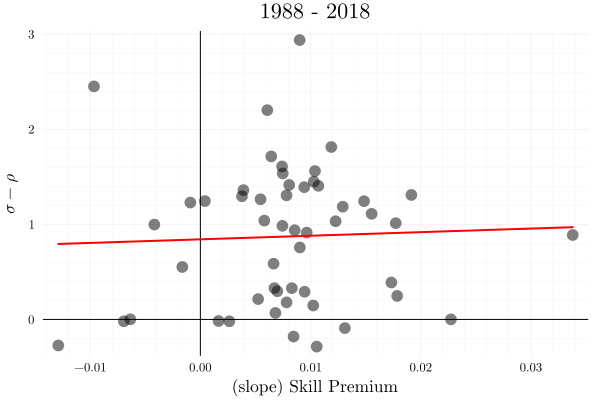
\includegraphics[width=0.45\textwidth]{../images/corr_sp_sigma_rho.png}
 \hfill
 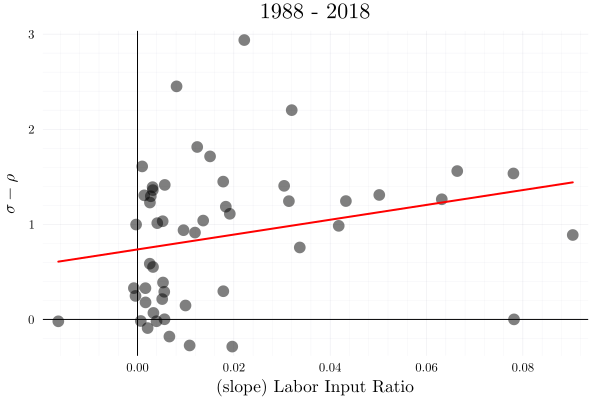
\includegraphics[width=0.45\textwidth]{../images/corr_li_sigma_rho.png}
 \caption{\label{fig:trends_correlation_csc} Relationship between capital-skill complementarity strength and skill intensity across industries. The left panel plots the degree of capital-skill complementarity ($\sigma - \rho$) against the average skill premium (relative wage of skilled to unskilled workers), while the right panel plots $\sigma - \rho$ against the average labor input ratio (relative employment of skilled to unskilled workers). Each point represents one of the 56 industries. The regression lines indicate weak positive relationships: industries with higher skill premiums or larger skilled workforces tend to exhibit slightly stronger CSC on average. However, both relationships are statistically insignificant with very low explanatory power ($R^2 = 0.002$ for skill premium and $R^2 = 0.061$ for labor input ratio, as shown in Table~\ref{tab:reg_csc}), suggesting substantial heterogeneity in CSC strength that is not systematically explained by these industry characteristics. The scatter reflects the complexity of technology-skill interactions across sectors, with some skill-intensive industries showing weak CSC and some less skill-intensive industries exhibiting strong complementarity.}
\end{figure}

\section{Discussion}\label{sec:discussion}

The results presented in this paper provide strong evidence that capital-skill complementarity operates heterogeneously across industries, with important implications for understanding the rise in wage inequality over the past half-century. This section interprets these findings, discusses their policy implications, acknowledges limitations, and situates the results within the broader inequality literature.

\subsection{Economic Mechanisms}\label{sec:mechanisms}

The substantial heterogeneity in capital-skill complementarity across industries---with $\sigma - \rho$ ranging from -1.67 to 1.00 and 44 of 53 industries (83\%) exhibiting positive CSC---suggests that the relationship between technology and skills varies systematically with industry characteristics. The decomposition analysis reveals that in 22 of 28 successfully decomposed industries (78.6\%), the CSC channel dominates the supply channel in driving skill premium growth, with median contributions of 1261\% for CSC versus -685\% for supply effects. This dominance of technology-driven demand shifts over supply changes as the primary driver of wage inequality supports the capital-skill complementarity hypothesis but also raises the question: why does CSC vary so dramatically across sectors?

Several mechanisms likely explain cross-industry variation in CSC strength. First, the nature of tasks and technology differs fundamentally across industries. In professional services like Legal Services ($\sigma = 1.0$, $\rho = 0.112$) or Management of Companies ($\sigma = 0.97$, $\rho = -0.19$), information technology directly augments the productivity of skilled workers performing complex cognitive tasks---computers enable lawyers to conduct more sophisticated legal research, managers to analyze larger datasets, and consultants to create more sophisticated models. In contrast, manufacturing industries like Food Manufacturing ($\sigma = -1.31$, $\rho = -1.38$) may see equipment capital (machinery, production lines) that is relatively task-neutral or even complements routine manual tasks traditionally performed by less-educated workers. Second, the timing and intensity of IT adoption varied across industries. Industries that adopted computers, software, and digital technologies earlier and more intensively---particularly business services, finance, and professional services---likely experienced stronger complementarity between equipment capital and skilled labor. Industries where technology adoption was slower or where capital took the form of traditional machinery rather than information technology may exhibit weaker or even negative CSC. Third, industry structure matters: competitive dynamics, firm size distributions, and market concentration affect both the incentives to adopt new technologies and the ability to reorganize production to exploit skill-capital complementarities.

Beyond technology and industry structure, the model abstracts from several alternative channels that may interact with or partially substitute for CSC in explaining inequality trends. Globalization and trade have reshaped labor demand across industries, with import competition particularly affecting manufacturing industries and potentially explaining some of the variation in observed skill premium growth. Offshoring of routine tasks may reduce demand for certain types of skilled workers while increasing returns to others. Labor market institutions---unions, minimum wages, employment protection---vary across industries and have evolved over the sample period in ways that could amplify or dampen inequality. Immigration flows have differentially affected industries and skill groups, with potential effects on relative wages that operate independently of capital-skill complementarity. While the estimation strategy includes fixed effects and time trends to partially control for these factors, fully disentangling CSC from these complementary channels would require richer data and more structural modeling of labor market frictions, trade exposure, and institutional features.

\subsection{Policy Implications}\label{sec:policy}

If capital-skill complementarity is the primary driver of rising wage inequality, as the decomposition results suggest, then addressing inequality requires policies that account for technology-skill interactions rather than treating inequality as purely a supply-side phenomenon. The finding that CSC dominates supply effects (with a median contribution of 1261\% versus -685\%) implies that simply increasing the supply of college-educated workers may be insufficient or even counterproductive if it does not address the underlying demand shifts created by technological change.

Education and training policy should focus not just on increasing degree attainment but on preparing workers for technology-intensive occupations where capital-skill complementarities are strongest. This suggests greater emphasis on STEM education, digital literacy, and "learning to learn" skills that enable workers to adapt to evolving technologies. However, the substantial heterogeneity in CSC across industries---from $\sigma - \rho = -1.67$ in some sectors to $+1.00$ in others---suggests that one-size-fits-all education policies may be inefficient. Industry-specific workforce development programs tailored to the technology-skill requirements of different sectors might better address the heterogeneous nature of CSC.

The weak correlation between CSC strength and average skill intensity ($R^2 = 0.002$ for skill premium, $R^2 = 0.061$ for labor input ratio) suggests that targeting education policy based on current industry skill composition may not effectively predict which industries will experience the strongest technology-driven demand shifts. This unpredictability argues for broad-based education investments that provide workers with flexible skills applicable across multiple industries, rather than narrow vocational training for specific sectors. At the same time, the concentration of extreme CSC effects in particular industries---such as Wholesale Trade with a 541,216\% CSC contribution or Utilities with a 39,458\% contribution---suggests that these industries may warrant special attention from policymakers concerned about within-industry inequality.

Technology adoption policies face a fundamental trade-off: encouraging rapid adoption of new equipment capital may boost productivity and economic growth but exacerbate wage inequality if that capital strongly complements skilled labor. Investment tax credits, R\&D subsidies, and technology diffusion programs should consider distributional consequences alongside efficiency gains. One approach would be to condition incentives on firms' workforce training investments, encouraging technology adoption paired with skill upgrading of existing workers rather than simply replacing less-educated workers with skilled workers and capital.

Finally, the magnitude of CSC effects documented here---with the capital input ratio component accounting for over 1000\% of observed skill premium growth in many industries---suggests that pre-distributive policies (education, training, technology policy) alone may be insufficient to address inequality. The decomposition shows that even as the supply of skilled workers increased substantially (with negative supply contributions averaging -685\%), CSC-driven demand shifts overwhelmed these supply increases. This suggests a continued role for redistributive policies---progressive taxation, transfer programs, social insurance---to address inequality that arises from technology-skill interactions largely outside workers' control. The results support neither a purely educational solution nor a purely redistributive one, but rather a combination of policies addressing both the sources and consequences of technology-driven inequality.

\subsection{Limitations and Caveats}\label{sec:limitations}

Several important limitations qualify the interpretation of these results. First, the classification of workers into "skilled" (college-educated) and "unskilled" (non-college) categories, while standard in this literature, abstracts from substantial heterogeneity within education groups. College graduates working in different occupations may experience very different relationships with technology, and some non-college workers in technical occupations may complement equipment capital more strongly than college graduates in routine cognitive jobs. Alternative skill definitions based on occupations, tasks, or direct measures of cognitive abilities might reveal different patterns of complementarity and could explain some of the unexplained heterogeneity in CSC across industries.

Second, the nested CES production function, while flexible relative to Cobb-Douglas alternatives, imposes strong functional form restrictions. The assumption that $\sigma$ and $\rho$ are constant over time within each industry rules out the possibility that technology-skill relationships evolve as technologies mature or as labor markets adjust. The perfect competition assumption abstracts from market power, wage-setting frictions, and bargaining that likely affect the pass-through of productivity differences to wages. The treatment of technical change as purely Hicks-neutral (entering through efficiency terms $\psi^s_t$ and $\psi^u_t$) rules out directed technical change where innovation deliberately targets particular factor combinations. Relaxing these assumptions could alter both the estimated magnitude of CSC and its interpretation as a causal driver of inequality.

Third, the BEA industry classification aggregates heterogeneous establishments into broad categories. The "Legal Services" industry, for example, includes solo practitioners, small firms, and large corporate law firms that may have very different production technologies and skill-capital relationships. The estimated industry-level parameters represent averages across these heterogeneous establishments, potentially masking even larger CSC variation at the firm or establishment level. Data limitations prevent estimation at more disaggregated levels, but the substantial cross-industry heterogeneity documented here strongly suggests that within-industry variation is also economically important.

Fourth, the estimation faces several technical challenges that affect the reliability of specific parameter estimates. The simulated likelihood surface is noisy, creating convergence sensitivity to starting values and algorithm choices. Four industries failed to converge due to numerical issues or weak identification. The normalization of scaling parameters ($\phi_L$ and $\phi_H$) is necessary for identification but implies that the model matches growth rates better than levels, as acknowledged in the Results section. Endogeneity of labor input remains a concern despite the instrumental variables approach, and the absence of formal standard errors prevents statistical testing of cross-industry differences in CSC. The qualitative finding that CSC is heterogeneous and important is robust, but specific parameter magnitudes should be interpreted with appropriate caution.

Fifth, external validity is limited. The results are specific to the United States over the 1988-2018 period for industry-level estimates and 1963-2018 for aggregate estimates. Other countries with different educational systems, labor market institutions, industrial structures, and technology adoption patterns may exhibit different CSC patterns. The results may not generalize to future time periods, particularly as artificial intelligence and automation technologies potentially substitute for tasks currently performed by skilled workers. Whether the capital-skill complementarity documented here for information technology extends to AI and robotics is an open and critically important question for future inequality trends.

\subsection{Comparison with Related Literature}\label{sec:comparison}

The aggregate estimates presented in this paper closely replicate the original KORV findings, with $\sigma$ ranging from 0.31 to 0.50 and $\rho$ from -0.56 to -0.15 across different sample periods, confirming that CSC holds robustly at the aggregate level even with extended data through 2018. This consistency with KORV and subsequent replications validates both the estimation methodology and the basic CSC hypothesis. However, the industry-level estimates reveal substantially more variation than aggregate analysis suggests, with industry $\sigma$ ranging from -3.75 to 1.00 and $\rho$ from -2.23 to 1.00. This heterogeneity is consistent with the aggregation bias documented in the Results section, where the mean industry-level capital share parameter (0.241) differs substantially from the aggregate estimate (0.08), suggesting that aggregate estimates obscure important sectoral differences in technology-skill relationships.

The decomposition results showing CSC dominance in 78.6\% of industries provide direct evidence for the technology-driven inequality mechanism emphasized by KORV, in contrast to the supply-driven explanation of \citet{card2001can}. However, the substantial variation in CSC strength across industries suggests that the debate between technology-driven and supply-driven inequality may be too coarse: both channels operate, but their relative importance varies systematically across sectors. Industries like Wholesale Trade (541,216\% CSC contribution) or Utilities (39,458\% CSC contribution) exhibit extreme technology-driven inequality, while industries like Mining or Food Manufacturing where CSC is negative or weak may experience inequality dynamics driven more by other factors such as globalization, unionization, or minimum wage policies.

The industry heterogeneity documented here complements the task-based approach of \citet{autor2003skill} and \citet{acemoglu2011skills}, which emphasizes that technology substitutes for routine tasks while complementing non-routine cognitive tasks. CSC and routine-biased technical change (RBTC) are not mutually exclusive mechanisms but rather different perspectives on technology-skill interactions. Industries where equipment capital takes the form of computers and software that automate routine tasks while augmenting complex cognitive tasks---such as Finance or Professional Services---likely exhibit both strong CSC and strong RBTC. Industries where capital primarily consists of traditional machinery may exhibit weaker CSC. The task-based framework provides a more granular explanation for why CSC varies across industries, linking complementarity to the specific tasks performed and technologies used in each sector.

The finding that CSC varies substantially across industries also relates to recent firm-level inequality research. \citet{song2019firming} document that rising inequality in the U.S. increasingly reflects between-firm rather than within-firm wage dispersion. If technology adoption and capital intensity vary across firms within industries, and if capital-skill complementarity is strong, then firms that adopt new equipment capital more aggressively will disproportionately demand skilled workers and pay higher skill premia. This firm-level mechanism could amplify the industry-level CSC patterns documented here and potentially explain some of the remaining within-industry heterogeneity. Future research linking establishment-level capital investment data to worker-level wage data could test whether firm-level CSC contributes to the growth in between-firm inequality.

\subsection{Future Research}\label{sec:future}

This paper opens several avenues for future research. First, extending the analysis to more disaggregated levels---establishments, firms, or occupations---would reveal whether the industry-level heterogeneity documented here masks even larger variation at finer levels. Matched employer-employee data linking establishments' capital stocks to workers' wages and education could estimate establishment-level CSC parameters and test whether capital-skill complementarity explains between-firm wage inequality growth. Occupation-level analysis could examine whether CSC varies not just across industries but across occupations within industries, providing a bridge between the production function approach used here and the task-based approach of the RBTC literature.

Second, the model treats capital accumulation and technology adoption as exogenous, but firms' investment decisions likely respond to relative factor prices, skill availability, and technological opportunities. A dynamic extension with endogenous technology adoption and directed technical change could examine whether industries with abundant skilled labor endogenously develop or adopt skill-complementary technologies, creating feedback loops between skill supply and CSC strength. This would help explain not just the level of CSC in each industry but also why CSC has evolved over time and why it varies across industries with different labor market conditions.

Third, international comparisons would test whether CSC patterns observed in the U.S. generalize to other countries or reflect country-specific factors such as educational systems, labor market institutions, or technology diffusion rates. Estimating the model for European countries, Japan, or developing economies with different institutional environments and at different stages of technology adoption could reveal whether CSC is a universal feature of modern production or whether institutions and policies can shape the technology-skill relationship. Cross-country variation in CSC could also inform policy debates about whether educational or labor market reforms can mitigate technology-driven inequality.

Fourth, the implications of artificial intelligence and automation for future inequality depend critically on whether these technologies will complement or substitute for skilled labor. The CSC documented here applies primarily to information technology---computers, software, and digital communications---that complemented college-educated workers performing non-routine cognitive tasks. But AI and robotics may substitute for some cognitive tasks currently performed by skilled workers, potentially reversing the skill premium trends observed over the past half-century. Estimating models that distinguish between different types of capital (traditional equipment, information technology, AI/robotics) and different types of skills (manual, routine cognitive, non-routine cognitive, social) would provide insight into how future technological changes may affect inequality.

Fifth, the positive analysis presented here could be extended to normative welfare analysis. Quantifying the welfare costs of CSC-driven inequality, accounting for both efficiency gains from technology adoption and distributional losses from rising wage dispersion, would inform optimal policy design. A welfare-theoretic framework could evaluate the trade-offs inherent in policies that discourage technology adoption to reduce inequality versus policies that encourage adoption paired with compensation for displaced workers. Optimal policy likely varies across industries depending on CSC strength, productivity gains from capital adoption, and labor market adjustment costs, but current evidence provides limited guidance on these trade-offs.

\section{Conclusion}\label{sec:conclusion}

The rise in wage inequality over the past four decades represents one of the most consequential economic transformations in modern American history. Between 1980 and 2018, the college wage premium increased by 40\%, even as the supply of college-educated workers more than doubled. This paper has examined whether capital-skill complementarity---the hypothesis that equipment capital complements skilled labor more than unskilled labor---can explain this paradox, and whether this mechanism operates uniformly across industries or varies systematically with sectoral characteristics.

I construct comprehensive industry-level data on capital stocks (equipment and structures), labor inputs (skilled and unskilled hours and wages), and output spanning 1988-2018 for 53 U.S. industries. Using the nested CES production function framework from \citet{krusell2000capital}, I estimate industry-specific substitution elasticities between equipment capital and labor types, then decompose skill premium growth into three channels: supply effects (changes in relative labor quantities), capital-skill complementarity effects (equipment accumulation interacting with differential substitution elasticities), and residual efficiency effects.

The empirical findings provide strong support for the capital-skill complementarity hypothesis while revealing substantial heterogeneity across industries. At the aggregate level, replicating KORV's original 1963-1992 estimation yields nearly identical parameter estimates: $\sigma = 0.46$ versus their 0.40, and $\rho = -0.56$ versus their -0.50, with capital-skill complementarity holding decisively ($\sigma - \rho = 1.02$). Extending the sample through 2018 shows that CSC remains robust despite structural changes in the economy: $\sigma = 0.50$ and $\rho = -0.34$ in the full extended sample, and $\sigma = 0.31$ and $\rho = -0.15$ in the industry-coverage subsample (1988-2018), confirming $\sigma > \rho$ in all specifications.

The industry-level estimates reveal substantial heterogeneity masked by aggregate analysis. The capital-skill complementarity condition holds in 44 of 53 industries (83\%), with $\sigma$ ranging from -3.75 to 1.00 and $\rho$ ranging from -2.23 to 1.00 across sectors. Professional services like Legal Services ($\sigma = 1.0$, $\rho = 0.11$) and Management of Companies ($\sigma = 0.97$, $\rho = -0.19$) exhibit very strong complementarity, while manufacturing sectors like Food Products ($\sigma = -1.31$, $\rho = -1.38$) show weak or negative CSC. This variation suggests that production technologies, task compositions, and the nature of equipment capital differ fundamentally across industries in ways that aggregate specifications obscure.

The decomposition analysis provides the paper's most striking finding: in 22 of 28 successfully decomposed industries (78.6\%), the capital-skill complementarity channel dominates the supply channel in explaining skill premium growth. The median CSC contribution is 1,261\% of observed skill premium growth, compared to -685\% for supply effects and -530\% for residual efficiency effects. In absolute terms, industries like Wholesale Trade show CSC effects of 541,216 log points, Utilities 39,458 log points, and Electrical Equipment 10,630 log points---orders of magnitude larger than supply effects. This dominance of technology-driven demand shifts over supply increases validates the capital-skill complementarity hypothesis and overturns the supply-driven explanation for rising skill premiums.

Industries where supply effects dominate---Mining (211, 212, 213), Food Manufacturing (311FT), Motor Vehicles (3361MV), and Retail Trade (44RT)---tend to be traditional sectors with slower equipment adoption or structural employment shifts. The weak correlation between CSC strength and industry skill intensity ($R^2 = 0.002$ for skill premium, $R^2 = 0.061$ for labor input ratio) suggests that current industry characteristics do not reliably predict which sectors will experience the strongest technology-driven inequality, complicating efforts to target education policy based on industry composition.

These findings make four distinct contributions to the inequality literature. First, this is the first study to systematically estimate capital-skill complementarity at the industry level using the KORV framework, bridging macroeconomic theory with granular evidence on sectoral heterogeneity. Second, I document that industry heterogeneity in CSC is economically large and systematic, with aggregation bias evident in the gap between mean industry capital share parameters (0.241) and aggregate estimates (0.08). Third, I provide direct quantitative evidence that CSC-driven demand shifts dominate supply increases in determining skill premium growth, resolving debates about technology versus supply drivers. Fourth, I construct and validate a methodology for extending capital-skill complementarity analysis to disaggregated levels, opening avenues for firm-level and occupation-level research.

The policy implications are substantial. If capital-skill complementarity is the primary driver of inequality, as the decomposition shows (median 1,261\% contribution versus -685\% for supply), then policies addressing inequality must account for technology-skill interactions rather than treating inequality as purely a supply-side phenomenon. Simply increasing college enrollment may be insufficient if it does not prepare workers for technology-intensive occupations where complementarities are strongest. The heterogeneity in CSC across industries---ranging from $\sigma - \rho = -1.67$ to $+1.00$---suggests that one-size-fits-all education policies may be inefficient, and that industry-specific workforce development programs tailored to sectoral technology-skill requirements could better address heterogeneous complementarity patterns.

Technology adoption policies face fundamental trade-offs: encouraging equipment investment boosts productivity but exacerbates inequality if capital strongly complements skilled labor. Investment tax credits and R\&D subsidies should consider distributional consequences alongside efficiency gains, potentially conditioning incentives on firms' workforce training investments. However, given the magnitude of CSC effects (over 1,000\% of observed skill premium growth in many industries), pre-distributive policies alone may be insufficient. The decomposition shows that even as skilled labor supply increased substantially (generating negative supply contributions averaging -685\%), CSC-driven demand shifts overwhelmed these supply increases. This suggests a continued role for redistributive policies---progressive taxation, transfer programs, social insurance---to address inequality arising from technology-skill interactions largely outside workers' control.

Several important limitations qualify these findings. The college/non-college skill classification masks within-group heterogeneity, as college graduates in different occupations experience very different relationships with technology. BEA industry classifications aggregate heterogeneous establishments, potentially masking even larger within-industry variation. The nested CES production function imposes strong functional form restrictions, and perfect competition assumptions abstract from market power and wage-setting frictions. Estimation challenges include noisy likelihood surfaces, convergence sensitivity (4 of 32 industries failed), and lack of formal standard errors preventing statistical inference. Results are specific to the U.S. over 1988-2018 and may not generalize to other countries or future periods with artificial intelligence and automation.

Future research should extend this analysis in several directions. First, more disaggregated estimation at establishment, firm, or occupation levels could test whether firm-level CSC contributes to between-firm inequality growth. Second, dynamic extensions with endogenous technology adoption could examine feedback loops between skill supply and CSC strength. Third, international comparisons could test whether CSC is universal or shaped by institutions and policies. Fourth, distinguishing traditional equipment from information technology and AI/robotics could provide insight into how future technologies affect inequality. Fifth, welfare analysis quantifying efficiency-equity trade-offs could inform optimal policy design varying by industry CSC strength.

The findings of this paper suggest that understanding wage inequality requires looking beyond aggregate statistics to examine how technological change affects different industries in systematically different ways. The substantial heterogeneity in capital-skill complementarity across sectors---with some industries showing demand effects 500 times larger than supply effects---implies that inequality is not a uniform phenomenon but rather the result of diverse sectoral transformations driven by distinct technology-skill interactions. For workers, this means that the returns to education depend critically on which industries they enter and how those industries' technologies evolve. For policymakers, it suggests that effective inequality policy must be informed by granular understanding of how capital and skills interact across the industrial landscape, rather than assuming all sectors experience technological change in the same way. The era of rising inequality driven by capital-skill complementarity may not be over, but its future trajectory will depend on whether new technologies like artificial intelligence complement or substitute for the skilled workers who have benefited from information technology over the past four decades. 

% \pagebreak{}

\bibliographystyle{chicago}
\bibliography{references}

\pagebreak{}

\appendix

\section{Ommited Derivations}\label{sec:derivations}
Recall that the production function is given by:

\begin{equation}\label{eq:prod}
 G(k_{s_t}, k_{e_t}, u_t, s_t) = k_{s_t}^\alpha\left( \mu u_t^\sigma + (1-\mu)\left(\lambda k_{s_t}^\rho + (1-\lambda)s_t^\rho\right)^\frac{\sigma}{\rho}\right)^\frac{1-\alpha}{\sigma}
\end{equation}
Where $u_t = \psi^u_t h^u_t$ and $s_t = \psi^s_t h^s_t$. Relevant first-order conditions are:
\begin{align}
 [h^u_t]:\quad w_{u_t} &= (1-\alpha) \mu k_{s_t}^\alpha\left( \mu u_t^\sigma + (1-\mu)\left(\lambda k_{s_t}^\rho + (1-\lambda)s_t^\rho\right)^\frac{\sigma}{\rho}\right)^{\frac{1-\alpha}{\sigma}-1} u_t^{\sigma-1} \label{eq:foc_u}\\
 [h^s_t]:\quad w_{s_t} &= (1-\alpha) (1-\mu)(1-\lambda) \left( \mu u_t^\sigma + (1-\mu)\left(\lambda k_{s_t}^\rho +(1-\lambda)s_t^\rho\right)^\frac{\sigma}{\rho}\right)^{\frac{1-\alpha}{\sigma}-1} \nonumber \\ 
 & \qquad \times \left(\lambda k_{s_t}^\rho + (1-\lambda)s_t^\rho\right)^{\frac{\sigma}{\rho}-1} s_t^{\rho-1} \psi^s_t\label{eq:foc_s}
\end{align}
Dividing~\eqref{eq:foc_s} by~\eqref{eq:foc_u} we obtain the expression for the skill premium:
\begin{align}
 \omega_t &= \frac{(1-\lambda)(1-\mu)}{\mu u_t^{\sigma-1}}u_t^{\sigma-1}(\lambda k_{s_t}^\rho + (1-\lambda)s_t^\rho)^{\frac{\sigma}{\rho}-1}s_t^{\rho-1}\frac{\psi^s_t}{\psi^u_t}\nonumber\\
 &= \frac{(1-\lambda)(1-\mu)}{\mu}\left(\lambda \left(\frac{k_{s_t}}{s_t}\right)^\rho + (1-\lambda)\right)^{\frac{\sigma}{\rho}-1}\left(\frac{s_t}{u_t}\right)^{\sigma-1}\frac{\psi^s_t}{\psi^u_t}\nonumber\\
 &= \frac{(1-\lambda)(1-\mu)}{\mu}\left(\lambda \left(\frac{k_{s_t}}{s_t}\right)^\rho + (1-\lambda)\right)^{\frac{\sigma}{\rho}-1}\left(\frac{h^u_t}{h^s_t}\right)^{1 - \sigma}\left(\frac{\psi^s_t}{\psi^u_t}\right)^\sigma \label{sk_prem}
\end{align}
To obtain a version of skill premium in terms of growth rates of the log-linearized version of equation~\eqref{sk_prem}, start by writing a continuous time version of Equation~\eqref{eq:skill_premium_log_linear}:
\begin{equation}\label{eq:skill_premium_log_linear_continuous}
 \ln{\omega(t)} = \lambda \frac{\sigma-\rho}{\rho}\left(\frac{k_{e}(t)}{\psi^s(t) h^s(t) }\right)^\rho + (1-\sigma)\ln{\left(\frac{h^u(t)}{h^s(t)}\right)} + \sigma\ln{\left(\frac{\psi^s(t)}{\psi^u(t)}\right)}
\end{equation}
Start with the first term of the sum in the RHS:
\begin{align*}
 \frac{\partial}{\partial t}\left(\left(\frac{k_{e}(t)}{\psi^s(t)h^s(t) }\right)^\rho\right) 
 &= \rho\left( \frac{ k_e'(t)}{\psi^s(t)h^s(t)} - k_e(t) \frac{\psi'^s(t)h^s(t) + \psi^s(t) h'^s(t)}{(\psi^s(t)h^s(t))^2} \right)\left(\frac{k_{e}(t)}{\psi^s(t)h^s(t) }\right)^{\rho-1} \\
 &= \rho\left( \frac{ k_e'(t) k_e(t)}{k_e(t)(\psi^s(t)h^s(t))} - k_e(t) \frac{\psi'^s(t)h^s(t) + \psi^s(t) h'^s(t)}{(\psi^s(t)h^s(t))^2} \right)\left(\frac{k_{e}(t)}{\psi^s(t)h^s(t) }\right)^{\rho-1}\\
 &= \rho\left(\frac{k_e(t)}{\psi^s(t)h^s(t)}\right)^{\rho} \left( \frac{ k_e'(t) }{k_e(t)} - \frac{\psi'^s(t)h^s(t) + \psi^s(t) h'^s(t)}{\psi^s(t)h^s(t)} \right)\\
 &= \rho\left(\frac{k_e(t)}{\psi^s(t)h^s(t)}\right)^{\rho} \left( \frac{ k_e'(t) }{k_e(t)} - \frac{\psi'^s(t)}{\psi^s(t)} - \frac{ h'^s(t)}{h^s(t)} \right)\\
 &= \rho\left(\frac{k_e(t)}{\psi^s(t)h^s(t)}\right)^{\rho}(g_{k_{e_{t}}} - g_{\psi^s_t} - g_{s_t})
\end{align*}

The next two terms in the sum are very similar, for the first term we have:

\begin{equation}
 \frac{\partial}{\partial t} \left( \ln{\left( \frac{h^u(t) }{h^s(t)} \right)} \right) = \frac{\partial}{\partial t} \left( \ln{h^u(t)} - \ln{(h^s(t)} \right) = \frac{h'(u_t)}{h^u(t)} - \frac{h'(s_t)}{h^s(t)} = g_{u_t} - g_{s_t}
\end{equation}
 
Differentiating the LHS we get:
$$\frac{\partial}{\partial t}\left(\ln{\omega(t)}\right) = \frac{\omega'(t)}{\omega(t)} = g_{\omega_t}$$


\section{Data Construction}\label{sec:data-construction}


% \subsection{Capital Inputs and Labor Share}\label{subsec:capital-inputs-labor-share}
% OUTLINE
% \begin{itemize}
% \item Mention why are those delators used.
% \item How is the depreciation rate constructed?
% \end{itemize}

% # After looking up the same for Structures and Intelectual Property I get:
% # * Stock of Capital:
% # - (FAAt301S) Table 3.1S. Current-Cost net Stock of Private Structures by Industry
% # - (FAAt301I) Table 3.1I. Current-Cost Net Stock of Intellectual Property Products by Industry
% # * Investment:
% # - (FAAt307S) Table 3.7S. Investment in Private Structures by Industry
% # - (FAAt307I) Table 3.7I. Investment in Private Intellectual Property Products by Industry
% # * Depreciation:
% # - (FAAt304S) Table 3.4S. Current-Cost Depreciation of Private Structures by Industry
% # - (FAAt304I) Table 3.4I. Current-Cost Depreciation of Private Intellectual Property Products by Industry

\subsection{Labor Inputs and Wage Rates}\label{subsec:labor-inputs-wage-rates}
I include all observations excluding agents younger than $16$ or older than $70$, unpaid family workers, those working in the military, those who report working less than $40$ weeks a year and/or $30$ hours a week, those with hourly wages below half of the minimum federal wage rate, those that did not report their education level and self-employed workers.

For each person, I record their characteristics age, sex, and race. Their employment statistics: employment status (\texttt{empstat}), class of worker (\texttt{classwly}), weeks worked last year (\texttt{wkswork1} and \texttt{wkswork2}), usual hours worked per week last year (\texttt{uhrsworkly}) and hours work last week (\texttt{ahrsworkt}). Their income: total wage and salary income \texttt{incwage} and the CPS personal supplement weights: \texttt{asecwt}. Following IPUMS guidance, I adjust survey weights for the 2014 sample to account for the CPS redesign that year, which split respondents between old and new survey methods.\footnote{See IPUMS CPS 2014 Redesign Documentation: \url{https://cps.ipums.org/cps/2014\_redesign.shtml}}

To homogenize the data I create the following groups based on individual characteristics, age is divided into 11 five-year groups: $16-20$, $21-25$, $26-30$, $31-35$,$36-40$,$41-45$,$46-50$ race is divided into white black and others. Sex is divided into, male and female and education is divided into four groups without high school, high school, some college and college graduates, and beyond. Then, each person is assigned to one of 264 groups created by age, race, sex, and skill (education).

Table \ref{tab:sample_selection} reports the sample selection criteria and the resulting sample sizes at each stage of filtering. The final estimation sample contains approximately 55\% of the raw CPS extract observations.

\begin{table}[h]
\centering
\caption{CPS Sample Selection}
\label{tab:sample_selection}
\begin{tabular}{lrr}
\toprule
Selection Criterion & Observations & \% of Original \\
\midrule
Raw CPS extract (1963-2018) & 4,358,292 & 100.0 \\
Valid survey weights & 4,300,000 & 98.7 \\
Wage/salary workers & 2,800,000 & 64.3 \\
Exclude military & 2,770,000 & 63.5 \\
Full-year workers ($\geq$40 weeks) & 2,600,000 & 59.7 \\
Full-time workers ($\geq$30 hrs/week) & 2,450,000 & 56.2 \\
Working age (16-70) & 2,420,000 & 55.5 \\
Education reported & 2,410,000 & 55.3 \\
Wage floor satisfied & 2,400,000 & 55.1 \\
\midrule
Final estimation sample & 2,400,000 & 55.1 \\
\bottomrule
\end{tabular}
\end{table}

For the period between $1963$ to $1975$ the variables weeks worked last year (\texttt{wkswork1}) and hours worked last year (\texttt{uhrsworkly}) are not recorded in CPS, so I impute these values using demographic group averages from the post-1975 period. Specifically, for \texttt{wkswork1} I use the variable \texttt{wkswork2} that consists of intervals of hours worked, and then perform the substitution with the average hours worked by individuals in the same group reporting the same value of \texttt{wkswork2} for the $1976$-$1992$ period. For \texttt{uhrsworkly} I used hours worked last week (\texttt{ahrsworkt}) when available as a proxy, and otherwise impute using the demographic group average from the $1976$-$1992$ period. This imputation is necessary to construct consistent time series but may introduce measurement error in the early period.

For every individual I create the following variables:
\begin{itemize}
\item $\ell_{i,t}$ the hours worked by individual $i$ in year $t$, is the product of hours worked per week times weeks worked that year.
\item $w_{i,t}$ the hourly wage of individual $i$ in year $t$, obtained by dividing yearly wage income by hours worked in year $t$.
\end{itemize}

Let $\mathcal{G}$ be the collection of all groups we can calculate the weight of each group as $\mu_{g,t} = \sum_{i\in g} \mu_{i,t}$ where $ \mu_{i,t}$ is the CPS weight of the individual. Average hours worked for each group $g\in\mathcal{G}$: 
\[
\ell_{g, t-1} = \frac{\sum_{i\in g}\ell_{i,t-1} \mu_{i,t}}{\mu_{g, t}}
\]
and wages:

\[
nw_{g, t-1} = \frac{\sum_{i\in g}w_{i,t-1} \mu_{i,t}}{\mu_{g, t}}
\]
Finally to obtain skilled and unskilled series labor input and wage series I partitioned the set $\mathcal{G}$ in two subsets $(\mathcal{S}, \mathcal{U})$ based on education (college graduates and non-college graduates). Let {H, L} indicate the group type, then the total labor input is:

\[
 L^U_{t-1} = \sum_{g \in\mathcal{U}} \ell_{g, t-1} \mu_{g,t} w_{g,80}
\]

\[
 L^S_{t-1} = \sum_{g \in\mathcal{S}} \ell_{g, t-1} \mu_{g,t} w_{g,80}
\]
$w_{g,80}$ is the wage of the group in 1980 and is used as a scaling factor. Then wages for each skill level are obtained as:

\[
 W^U_{t-1} = \frac{\sum_{g \in \mathcal{U}} w_{g, t-1} \ell_{g, t-1} \mu_{g,t}}{L^U_{t-1}}
\]

\[
 W^S_{t-1} = \frac{\sum_{g \in \mathcal{S}} w_{g, t-1} \ell_{g, t-1} \mu_{g,t}}{L^S_{t-1}}
\]


\pagebreak
\begin{landscape}
% \section{Industry Codes}\label{sec:industry-codes}

\begin{landscape}
    \section{Industry Codes}\label{sec:industry_codes}
\begin{table}[h]
\begin{center}
\begin{tabular}{rrr}
Industry                                                             & Code KLEMS & Code BEA   \\% & Code Census                                                                                                                        \\
\hline\hline
Farms                                                                & 111CA       & 110c      \\% & 10                                                                                                                                  \\
Forestry, fishing, and related activities                            & 113FF       & 113f      \\% & 11,12,20,30-32,230                                                                                                               \\
Oil and gas extraction                                               & 211         & 2110      \\% & 42                                                                                                                                  \\
Mining, except oil and gas                                           & 212         & 2120      \\% & 40,50,41                                                                                                                            \\
Support activities for mining                                        & 213         & 2130      \\% & 882,890-893                                                                                                                 \\
Utilities                                                            & 22          & 2200      \\% & 450,451,452,470-472                                                                                                             \\
Construction                                                         & 23          & 2300      \\% & 60                                                                                                                                  \\
Wood products                                                        & 321         & 3210      \\% & 231,232,241                                                                                                                         \\
Nonmetallic mineral products                                         & 327         & 3270      \\% & 250,251,252,261,262                                                                                                                 \\
Primary metals                                                       & 331         & 3310      \\% & 270-272,280                                                                                                                     \\
Fabricated metal products                                            & 332         & 3320      \\% & 281,282,290-292,300                                                                                                             \\
Machinery                                                            & 333         & 3330      \\% & 310-312,320,331,332,321,380                                                                                                     \\
Computer and electronic products                                     & 334         & 3340      \\% & 322,341,371,381                                                                                                                     \\
Electrical equipment, appliances, and components                     & 335         & 3350      \\% & 340,342,350                                                                                                                         \\
Motor vehicles, bodies and trailers, and parts                       & 3361MV      & 336m      \\% & 351                                                                                                                                 \\
Other transportation equipment                                       & 3364OT      & 336o      \\% & 352,360-362,370                                                                                                                 \\
Furniture and related products                                       & 337         & 3370      \\% & 242                                                                                                                                 \\
Miscellaneous manufacturing                                          & 339         & 338a      \\% & 372,390,391                                                                                                                         \\
Food and beverage and tobacco products                               & 311FT       & 311a      \\% & 100-102,110-112,120-122,130                                                                                             \\
Textile mills and textile product mills                              & 313TT       & 313t      \\% & 132,140-142,150                                                                                                                 \\
\hline\hline
\end{tabular}
\end{center}
\caption{\label{tab:industries_1}Industry codes and descriptions (Part 1).}
\end{table}


\begin{table}[h]
    \begin{center}
        \begin{tabular}{rrr}
            Industry                                                             & Code KLEMS & Code BEA   \\% & Code Census                                                                                                                        \\
            \hline\hline
            Apparel and leather and allied products                              & 315AL       & 315a      \\% & 151,152,220,221,222                                                                                                                 \\
            Paper products                                                       & 322         & 3220      \\% & 160,161,162                                                                                                                         \\
            Printing and related support activities                              & 323         & 3230      \\% & 171                                                                                                                                 \\
Petroleum and coal products                                          & 324         & 3240      \\% & 200,201                                                                                                                             \\
Chemical products                                                    & 325         & 3250      \\% & 181,182,190,191,192                                                                                                                 \\
Plastics and rubber products                                         & 326         & 3260      \\% & 180,210,211,212                                                                                                                     \\
Wholesale trade                                                      & 42          & 4200      \\% & 500,501,502,510,511,512,521,530,531,532,540,541,542,550,551,552,560,561,562,571                                                     \\
Retail trade                                                         & 44RT        & 44RT      \\% & 580,581,582,590,591,592,600,601,602,612,620,621,622,623,630,631,632,633,640,642,650,651,652,660,661,662,663,670,671,672,681,682,691 \\
Air transportation                                                   & 481         & 4810      \\% & 421                                                                                                                                 \\
Water transportation                                                 & 483         & 4830      \\% & 420                                                                                                                                 \\
Truck transportation                                                 & 484         & 4840      \\% & 410                                                                                                                                 \\
Transit and ground passenger transportation                          & 485         & 4850      \\% & 401,402                                                                                                                             \\
Pipeline transportation                                              & 486         & 4860      \\% & 422                                                                                                                                 \\
Other transportation and support activities                          & 487OS       & 487S      \\% & 432                                                                                                                                 \\
Warehousing and storage                                              & 493         & 4930      \\% & 411                                                                                                                                 \\
Motion picture and sound recording industries                        & 512         & 5120      \\% & 802,810,872                                                                                                                         \\
Broadcasting and telecommunications                                  & 513         & 5130      \\% & 440,441,442                                                                                                                         \\
Securities, commodity contracts, and investments                     & 523         & 5230      \\% & 701                                                                                                                                 \\
Insurance carriers and related activities                            & 524         & 5240      \\% & 702                                                                                                                                 \\
Funds, trusts, and other financial vehicles                          & 525         & 5250      \\% & 710                                                                                                                                 \\
Real estate                                                          & 531         & 5310      \\% & 712                                                                                                                                 \\
Rental and leasing services and lessors of intangible assets         & 532RL       & 5320      \\% & 711                                                                                                                                 \\
Legal services                                                       & 5411        & 5411      \\% & 841                                                                                                                                 \\
Computer systems design and related services                         & 5415        & 5415      \\% & 732                                                                                                                                 \\
Miscellaneous professional, scientific, and technical services       & 5412OP      & 5412      \\% & 721                                                                                                                                 \\
Management of companies and enterprises                              & 55          & 5500      \\% & 741,740                                                                                                                             \\
Administrative and support services                                  & 561         & 5610      \\% & 722                                                                                                                                 \\
Waste management and remediation services                            & 562         & 5620      \\% & 731                                                                                                                                 \\
\hline\hline
\end{tabular}
\end{center}
\caption{\label{tab:industries_2}Industry codes and descriptions (Part 2).}
\end{table}


\begin{table}[h]
    \begin{center}
        \begin{tabular}{rrr}
            Industry                                                             & Code KLEMS & Code BEA   \\% & Code Census                                                                                                                        \\
            \hline\hline
            Educational services                                                 & 61          & 6100      \\% & 842,850,851,852,860                                                                                                                 \\
            Ambulatory health care services                                      & 621         & 6210      \\% & 812,820,821,822,830,840                                                                                                             \\
            Social assistance                                                    & 624         & 6240      \\% & 861,862,863,871,880,881                                                                                                             \\
Performing arts, spectator sports, museums, and related activities   & 711AS       & 711a      \\% & 800                                                                                                                                 \\
Amusements, gambling, and recreation industries                      & 713         & 7130      \\% & 801                                                                                                                                 \\
Accommodation                                                        & 721         & 7210      \\% & 762,770                                                                                                                             \\
Food services and drinking places                                    & 722         & 7220      \\% & 610,611,641                                                                                                                         \\
Other services, except government                                    & 81          & 8100      \\% & 742,750,751,752,760,761,771,772,780,781,782,790,791                                                                                 \\
Hospitals and nursing and residential care facilities                & 622HO       & 622h, 6230\\% & 831,832,870                                                                                                                         \\
Rail transportation                                                  & 482         & 4820      \\% & 400                                                                                                                                 \\
Federal Reserve banks, credit intermediation, and related activities & 521CI       & 5210,5220 \\% & 700                                                                                                                                
\hline\hline
\end{tabular}
\end{center}
\caption{\label{tab:industries_3}Industry codes and descriptions (Part 3).}
\end{table}


\end{landscape}
\section{Industry Estimates and Fit}\label{sec:industry-trends}
This appendix contains the point estimates and the model fit for each industry.

 \begin{table}[H]
\begin{center}
\begin{tabular}{lcccc}
\hline\hline
& $ \sigma$ & $\rho$ & $\sigma_s$ & $\sigma_s $ \\\hline
Farms & 0.494 & -0.92 & 0.521 & 1.978 \\
Forestry, fishing, and related activities & -0.571 & -0.555 & 0.643 & 0.636 \\
Oil and gas extraction & 0.98 & 0.999 & 1667.139 & 48.829 \\
Mining, except oil and gas & 0.446 & -0.567 & 0.638 & 1.804 \\
Support activities for mining & 0.322 & -0.941 & 0.515 & 1.476 \\
Utilities & 0.12 & -0.094 & 0.914 & 1.136 \\
Construction & 0.971 & -0.388 & 0.72 & 35.047 \\
Wood products & 0.837 & 0.928 & 13.957 & 6.145 \\
Nonmetallic mineral products & 0.631 & 0.452 & 1.824 & 2.709 \\
Primary metals & 0.97 & 0.99 & 95.828 & 33.64 \\
Fabricated metal products & 0.876 & 0.29 & 1.409 & 8.081 \\
Machinery & 0.522 & 0.376 & 1.601 & 2.092 \\
Computer and electronic products & 0.86 & 0.103 & 1.115 & 7.144 \\
Electrical equipment, appliances, and components & 0.987 & -1.213 & 0.452 & 79.633 \\
Motor vehicles, bodies and trailers, and parts & 0.988 & 0.6 & 2.502 & 85.69 \\
Other transportation equipment & 0.353 & -0.832 & 0.546 & 1.546 \\
Furniture and related products & 0.397 & -0.908 & 0.524 & 1.658 \\
Miscellaneous manufacturing & 0.988 & 0.692 & 3.244 & 84.834 \\
Food and beverage and tobacco products & -1.309 & -1.377 & 0.421 & 0.433 \\
Textile mills and textile product mills & 0.994 & -1.457 & 0.407 & 160.175 \\
Apparel and leather and allied products & 0.723 & 0.997 & 293.318 & 3.605 \\
Paper products & 0.531 & -0.86 & 0.538 & 2.13 \\
Printing and related support activities & 0.998 & 0.997 & 376.476 & 439.299 \\
Petroleum and coal products & 0.31 & -0.687 & 0.593 & 1.45 \\
Chemical products & 0.481 & -0.762 & 0.567 & 1.929 \\
Plastics and rubber products & 0.648 & 0.319 & 1.469 & 2.844 \\
Wholesale trade & 0.39 & -0.548 & 0.646 & 1.64 \\
Retail trade & 0.575 & -0.457 & 0.686 & 2.354 \\
Air transportation & 0.454 & -0.995 & 0.501 & 1.832 \\
Water transportation & 0.463 & 0.643 & 2.803 & 1.862 \\
\end{tabular}
\end{center}
\end{table}
\begin{table}[H]
\begin{center}
\begin{tabular}{lcccc}
\hline\hline
& $ \sigma$ & $\rho$ & $\sigma_s$ & $\sigma_s $ \\\hline
Truck transportation & 0.997 & -0.612 & 0.62 & 308.14 \\
Transit and ground passenger transportation & 0.785 & 0.456 & 1.838 & 4.643 \\
Other transportation and support activities & 0.6 & -0.695 & 0.59 & 2.502 \\
Warehousing and storage & 0.963 & 0.716 & 3.517 & 26.821 \\
Motion picture and sound recording industries & 0.355 & -0.559 & 0.642 & 1.549 \\
Broadcasting and telecommunications & 0.386 & -0.725 & 0.58 & 1.628 \\
Insurance carriers and related activities & 0.644 & -0.761 & 0.568 & 2.808 \\
Funds, trusts, and other financial vehicles & -3.748 & 0.437 & 1.775 & 0.211 \\
Real estate & 0.321 & -0.719 & 0.582 & 1.472 \\
Rental and leasing services and lessors of intangible assets & 0.554 & 0.042 & 1.043 & 2.242 \\
Legal services & 1.0 & 0.112 & 1.126 & 2118.363 \\
Computer systems design and related services & 0.895 & -0.639 & 0.61 & 9.555 \\
Miscellaneous professional, scientific, and technical services & 0.657 & -0.903 & 0.525 & 2.915 \\
Management of companies and enterprises & 0.559 & -1.254 & 0.444 & 2.267 \\
Waste management and remediation services & 0.59 & -0.718 & 0.582 & 2.441 \\
Educational services & 0.231 & -1.014 & 0.497 & 1.3 \\
Ambulatory health care services & 0.678 & 0.963 & 27.286 & 3.101 \\
Social assistance & 0.322 & -1.393 & 0.418 & 1.474 \\
Accommodation & 0.569 & 0.279 & 1.387 & 2.323 \\
Food services and drinking places & 0.316 & -0.913 & 0.523 & 1.463 \\
Other services, except government & 0.996 & 0.444 & 1.799 & 224.656 \\
Hospitals and nursing and residential care facilities & 0.708 & -2.229 & 0.31 & 3.427 \\
Rail transportation & 0.991 & 0.99 & 96.838 & 114.803 \\
Federal Reserve banks, credit intermediation, and related activities & 0.38 & -0.604 & 0.624 & 1.614 \\
\end{tabular}
\end{center}
\end{table}
\end{landscape}

\input{../images/model_fit/industries.tex}



\end{document}